\documentclass[a4paper]{article}
\usepackage[fontsize=13pt]{scrextend}

% Hỗ trợ tiếng Việt
\usepackage[T5,TS1,T1]{fontenc} % 3 of lmodern's 8 encodings
\usepackage{lmodern}
\usepackage[utf8]{inputenc}
% \usepackage{mathptmx}
\usepackage[vietnamese]{babel}

% Các gói cần thiết
\usepackage{makecell}
\usepackage{parskip}
\usepackage{graphicx} 
\usepackage{xcolor}
\usepackage{tikz}
\usepackage{scrextend}
\usepackage{array}
\usepackage{float}
\usepackage{amsfonts}
\usepackage{amssymb}
\usepackage{siunitx}
\usepackage{booktabs}
\usepackage{caption}
\usepackage[version=4]{mhchem}
\usepackage{stmaryrd}
\usepackage{relsize}
\usepackage{fancyhdr} 
\usepackage{url}
\usepackage{setspace}
\usepackage{makecell}
\usepackage{enumitem}
\usepackage{changepage}
\usepackage{tabularx}
\usepackage[super]{nth}
\usepackage{listings}
\usepackage{courier}
\usepackage[titles]{tocloft}
\usepackage{longtable}
\usepackage{multirow}
\usepackage{circuitikz}
\usepackage{rotating}
\usepackage{hyperref}
\usepackage{subfiles}
\usepackage[style=english]{csquotes}
\usepackage{biblatex}
\usetikzlibrary{calc}
\usepackage{soul}
\usepackage{algorithm}
\usepackage{algpseudocode}
\usepackage{booktabs} % preamble
\usepackage{acro} 
% \usepackage{glossaries}

\usepackage{subfig}
% Thiết lập margin
\usepackage[left=3cm, right=2cm, top=2.5cm, bottom=3cm]{geometry}
\addbibresource{ref.bib}

% \setlength{\parindent}{1.5em}
\setstretch{1.3}
\setlength{\parskip}{6pt}
\setlength{\parindent}{1cm}
% Thiết lập hyperref
\hypersetup{
    colorlinks=true,
    linkcolor=black,
    filecolor=magenta,      
    urlcolor=cyan,
    pdftitle={},
    pdfauthor={},
}

\makeatletter
\renewcommand{\paragraph}{%
  \@startsection{paragraph}{4}{\z@}%
  {1.25ex \@plus 1ex \@minus .2ex}%
  {0.5em}%
  {\normalfont\normalsize\bfseries}%
}
\makeatother

\title{}
\author{Vũ Văn Minh}
\date{\today}

\acsetup{
  list/name = Danh mục từ viết tắt,
  list/preamble = \addcontentsline{toc}{section}{\acrolistname}
}

\DeclareAcronym{uav}{
  short = UAV,
  long  = Unmanned Aerial Vehicle,
  extra = Thiết bị bay không người lái
}
\DeclareAcronym{dtn}{
  short = DTN,
  long  = Delay/Disruption Tolerant Network,
  extra = Mạng chịu trễ
}
\DeclareAcronym{mfn}{
  short = MFN,
  long  = Message Ferry Network,
  extra = Mạng phà thông điệp
}



\begin{document}

% Places a dot after Chapter/Section/Subsection number in Table of Contents
\renewcommand{\appendixname}{Chương}
\renewcommand{\contentsname}{Mục lục}
\renewcommand{\listtablename}{Danh sách bảng biểu \addcontentsline{toc}{section}{Danh sách bảng biểu}}
\renewcommand{\listfigurename}{Danh sách hình ảnh \addcontentsline{toc}{section}{Danh sách hình ảnh}}
\renewcommand{\listalgorithmname}{Danh sách thuật toán \addcontentsline{toc}{section}{Danh sách thuật toán}}
\renewcommand{\tablename}{Bảng}
\renewcommand{\figurename}{Hình}

% Đổi tên caption "Algorithm"
\floatname{algorithm}{Thuật toán}
% Đổi Require / Ensure
\algrenewcommand\algorithmicrequire{\textbf{Đầu vào:}}
\algrenewcommand\algorithmicensure{\textbf{Đầu ra:}}

% \newcommand{\myparagraph}[1]{\paragraph{#1}\mbox{}\\}
\renewcommand{\cftsecaftersnum}{.}
\renewcommand{\cftsubsecaftersnum}{.}
\renewcommand{\cftsecleader}{\cftdotfill{\cftdotsep}}
\newenvironment{zeroindent}
  {\par\setlength{\parindent}{0pt}}
  {\par}

\newenvironment{thankpage}{}{}
\newcommand{\quotes}[1]{``#1''}

\subfile{title.tex}
\subfile{title2.tex}
\subfile{thanks.tex}
\subfile{glossary.tex}

\phantomsection
\addcontentsline{toc}{section}{Tóm tắt}
\fontsize{13pt}{16.9pt}\selectfont  % 16.9 ≈ 1.3 line spacing

{\huge \bfseries {Tóm tắt}}

Trong bối cảnh thiên tai bão lũ thường xuyên xuất hiện, đặc biệt tại các tỉnh miền Trung Việt Nam, sự phát triển công nghệ cùng sự trỗi dậy của các thiết bị bay không người lái (UAV) đã mở ra một ý tưởng về việc sử dụng các UAV này để hỗ trợ truyền thông cho các nút mặt đất bị cô lập do hạ tầng mạng truyền thống bị phá hủy. 
Các UAV hoạt động như những người đưa thư, tận dụng cơ chế lưu trữ - mang theo - chuyển tiếp của mạng chịu trễ, bay giữa các nút mặt đất để gửi và nhận thông điệp. 
Các nghiên cứu trước đó như TaBaf, DTP-TSP-D, FPOD hay EPP đều tồn tại các hạn chế về quy hoạch lộ trình, và chúng cũng đều chưa đề cập đến việc trao đổi thông điệp giữa hai nút mạng ở mức giao thức. 
Vì vậy, với mục tiêu để có thể áp dụng triển khai trong thực tế, nghiên cứu này đề ra: một giao thức trao đổi thông điệp giữa hai nút mạng và một phương pháp quy hoạch lộ trình, định tuyến và lập lịch di chuyển 2 pha VH-mTSP-RE cho các UAV được xây dựng bằng các thuật toán tối ưu hóa.

Các thực nghiệm trên bộ mô phỏng ns-3 cho thấy VH-mTSP-RE đạt hiệu năng vượt trội về Tỷ lệ truyền thành công, Tỷ lệ giao tiếp kém và Tỷ lệ không thể giao tiếp so với các phương pháp đối chứng.

{\bfseries Từ khóa:} Optimization, Delay Tolerant Network, Message Ferry Network, UAV (Unmanned Aerial Vehicle), multiple Traveling Saleman Problem


\newpage
\begingroup
\centering
\tableofcontents
\endgroup

\newpage
\listoftables
\newpage
\listoffigures
\newpage
\listofalgorithms
\newpage
% The \ac{epa} and \ac{re} development 
% \acuseall
% \printacronyms

\newpage

% * Phần 1 ===============================================================
\section{Giới thiệu}
\subsection{Bối cảnh và mục tiêu nghiên cứu}
Trong các kịch bản hậu thảm họa, điển hình lũ lụt tại các tỉnh miền Trung Việt Nam, hạ tầng mạng truyền thống thường bị hư hại nghiêm trọng hoặc mất hoàn toàn, dẫn đến tình trạng các nút mạng bị cô lập. 
Các nút này có thể đại diện cho các cụm dân cư, trung tâm cứu hộ, hoặc các điểm trú ẩn tạm thời. Trong bối cảnh đó, nhu cầu trao đổi thông tin giữa các nút bị cô lập này trở nên cấp thiết, phục vụ cho công tác cứu hộ, điều phối nguồn lực và tiếp tế nhu yếu phẩm. 
Những thông tin này không chỉ là văn bản, mà còn có thể là hình ảnh, video,\dots

Sự phát triển của các thiết bị bay không người lái mở ra khả năng thiết lập một hạ tầng mạng tạm thời dựa trên mô hình mạng chịu trễ, trong đó UAV đóng vai trò như các người đưa thư, đi thu thập và truyền thông điệp giữa các nút bị cô lập.

Trong nghiên cứu này, bài toán thực tế được mô hình hóa như sau: một tập các nút mạng cố định và đôi một cô lập được phân bố trong khu vực thảm họa cần trao đổi thông điệp với nhau thông qua các UAV. Các thông điệp được sinh ra tại các nút theo thời gian và bị ràng buộc bởi thời gian sống (time-to-live - TTL).
Mỗi UAV di chuyển với tốc độ giới hạn và có dung lượng bộ đệm hữu hạn. Việc trao đổi giữa 2 nút mạng chỉ có thể thực hiện khi khoảng cách của hai nút nhỏ hơn bán kính liên lạc, và các UAV đóng vai trò trung gian duy nhất trong quá trình truyền tải.

Từ đó, bài toán đặt ra bao gồm các yêu cầu chính: 
\begin{itemize}
  \item Cần có giao thức để hai nút trong mạng có thể giao tiếp và trao đổi thông điệp với nhau.
  \item Cần quy hoạch lộ trình các UAV để ghé thăm tất các nút mặt đất nhằm thu thập và gửi thông điệp.
  \item Các UAV cần phối hợp với nhau để định tuyến và chuyển tiếp thông điệp trước khi chúng hết hạn, tối ưu hóa các tiêu chí như Tỉ lệ truyền thành công (Delivery Ratio), Tỉ lệ không thể giao tiếp (Dead Connection Ratio), Tỉ lệ giao tiếp kém (Low Connection Ratio) và Độ trễ trung bình (Average Delay of Top x\%).
  \item Toàn bộ hệ thống phải hoạt động hiệu quả dưới các ràng buộc về tài nguyên như dung lượng bộ đệm, số lượng UAV, thời gian sống của thông điệp, tốc độ của UAV, ...
\end{itemize}

Mục tiêu nghiên cứu của đề tài này gồm 2 phần chính, là đề xuất một giao thức trao đổi gói tin giữa các nút trong mạng và đi sâu vào việc quy hoạch lộ trình và định tuyến cho những ``người đưa thư'' uav. Đó là đề xuất thuật toán quy hoạch lộ trình, định tuyến thông điệp và lập lịch bay Virtual Hub m-Traveling Saleman Problem and Route Extend (VH-mTSP-RE) được xây dựng trên các thuật toán tôi ưu hóa. Kèm theo so sánh và đánh giá với các nghiên cứu trước đó trên các tiêu chí đã nêu. 

\subsection{Phạm vi và giới hạn của đề tài}
Khóa luận này tập trung vào việc phát triển giao thức trao đổi thông điệp, cơ chế quy hoạch lộ trình, định tuyến thông điệp và lập lịch bay VH-mTSP-RE và đánh giá chúng trên môi trường mô phỏng ns-3 nhằm so sánh với các phương án quy hoạch lộ trình và định tuyến thông điệp từ các nghiên cứu trước đó. Phạm vi của nghiên cứu bao gồm:

\begin{itemize}
  \item {\bfseries Miền ứng dụng:} Đề tài tập trung vào quy hoạch lộ trình, chuyển tiếp thông điệp và lập lịch bay cho các UAV và đề xuất giao thức trao đổi với mục tiêu hỗ trợ truyền thông điệp giữa các nút mạng bị cô lập, hướng đến triển khai trong thực tế.
  \item {\bfseries Phương pháp:} Khóa luận thiết kế một giao thức trao đổi thông diệp giữa 2 nút mạng và đề xuất phương án quy hoạch lộ trình, định tuyến thông điệp và lập lịch bay 2 pha ``Virtual Hub m-Traveling Saleman Problem and Route Extend'' (VH-mTSP-RE) áp dụng các thuật toán tối ưu hóa.
  \item {\bfseries Đối chứng và cấu hình thực nghiệm:} Các nút mặt đất bị cô lập được tạo ra ngẫu nhiên dựa trên quan sát từ thực tế. Đề tài so sánh VH-mTSP-RE với:
  \begin{itemize}
    \item SIRA / Single Route: baseline với các UAV di chuyển theo một lộ trình TSP qua tất cả các nút.
    \item DTP-TSP-D: một phương án sử dụng thông tin về hạn (deadline) của các thông điệp để quy hoạch lộ trình.
    \item TaBaf và FPOD: hai phương án này quy hoạch lộ trình của UAV một cách cơ hội, ngay trong khi đang thực hiện nhiệm vụ (on the fly) dựa trên khoảng cách, các thông điệp trong bộ đệm, thời gian phục vụ, ...
    \item VH-mTSP: Phiên bản chỉ sử dụng pha 1 trong quy hoạch lộ trình của đề xuất.
  \end{itemize}
  \item {\bfseries Đánh giá:} Để đánh giá hiệu năng của các phương pháp trong từng kịch bản, cần các thước đo như Delivery Ratio, Dead Connection Ratio, Low Connection Ratio và Average Delay of Top x\%.

\end{itemize}
Khóa luận này vẫn còn một số giới hạn:
\begin{itemize}
  \item {\bfseries Giới hạn mô phỏng:} Toàn bộ đánh giá được thực hiện trên bộ mô phỏng ns-3 và chỉ sử dụng các mô hình truyền dẫn đơn giản, không mô phỏng chính xác môi thực tế như nhiễu, vật cản, gió, thời tiết.
  \item {\bfseries Ngoài phạm vi:} 
  \begin{itemize}
    \item Các nút mặt đất trong mô phỏng được coi là các nút trừu tượng, tượng trưng cho một hoặc một nhóm nút gần nhau trong thực tế. Bài toán nhóm các nút trên mặt phẳng thành các vị trí đại diện tối ưu tương đương với bài toán Unit Disk Cover, nằm ngoài phạm vi của khóa luận. 
    \item Giao thức trao đổi chưa xét đến các yếu tố như bảo mật, độ tin cậy hay phân mảnh thông điệp.
    \item Nghiên cứu chưa xét đến khả năng va chạm giữa các UAV khi di chuyển trong thực tế.
  \end{itemize}
  \item {\bfseries Giả định mô hình:} Giao thức trao đổi đề xuất dựa trên giả định rằng tất cả các thông điệp đều có độ lớn như nhau, và dung lượng bộ đệm của UAV được tính theo số thông điệp mà nó có thể lưu trữ.
  \item {\bfseries Giới hạn về khả năng:} Nghiên cứu chưa có cơ chế để có thể thêm hoặc bớt nút mạng trong thời gian chạy.
\end{itemize}

\subsection{Đóng góp chính của khóa luận}
Khóa luận trình bày một giải pháp tổng thể cho bài toán trao đổi thông điệp, quy hoạch lộ trình và định tuyến thông điệp giữa các nút mạng trong mạng phà thông điệp, hướng đến áp dụng vào thực tế khi các UAV hỗ trợ truyền thông hậu thảm họa:
\begin{itemize}
  \item Đề xuất giao thức trao đổi thông điệp giữa hai nút mạng. Khác với các nghiên cứu trước chủ yếu tập trung vào quy hoạch lộ trình và định tuyến thông điệp, giao thức này đóng vai trò như một nền tảng cho việc triển khai hệ thống vào thực tế.
  \item Đề xuất phương pháp quy hoạch lộ trình hai pha ``Hub m-Traveling Saleman Problem and Route Extend'' (H-mTSP-RE) được thực hiện bằng các thuật toán tối ưu hóa. Trong đó pha H-mTSP thực hiện phân chia nhiệm vụ cho các UAV một cách công bằng, đồng thời tìm một điểm trung chuyển tối ưu để các UAV tập hợp và trao đổi bằng việc giải một biến thể của bài toán tối ưu hôa mTSP kinh điển. Pha RE cải thiện lộ trình ban đầu bằng việc tận dụng thời gian rảnh của các UAV được phân ít công việc hơn để đi hỗ trợ, nâng cao hiệu quả của phương pháp.
  \item Đề xuất chiến lược trung chuyển ảo (Virtual Hub), trong đó các UAV thay vì dùng một nút mạng làm trung gian thì sẽ tập hợp tại điểm trung chuyển để trao đổi. Từ đó áp dụng chiến lược lên lộ trình tìm được trước đó để xây dựng thuật toán định tuyến và lập lịch bay của các UAV. Hoàn thiện đề xuất thành ``Virtual Hub m-Traveling Saleman Problem and Route Extend'' (VH-mTSP-RE).

  \item Cài đặt các thuật toán, tích hợp bộ mô phỏng ns-3 để có thể mô phỏng và thu thập các chỉ số đánh giá.
  \item Thực nghiệm và so sánh với các phương pháp hiện có, bao gồm phương pháp sử dụng deadline của các thông điệp (DTP-TSP-D) và các phương pháp tham lam dựa trên quan sát cục bộ (TaBaf, FPOD), chứng minh hiệu quả của VH-mTSP-RE về các chỉ số Delivery Ratio, Dead Connection Ratio và Low Connection Ratio
\end{itemize}

\subsection{Cấu trúc của khóa luận}
Cấu trúc của Khóa luận được chia thành 5 chương:
\begin{itemize}
  \item Chương 1 - Giới thiệu: Trình bày động lực, mục tiêu và phạm vi đề tài, đóng góp và cấu trúc tổng quan của khóa luận.
  \item Chương 2 - Cơ sở lý thuyết và nghiên cứu liên quan: Trình bày tổng quan về Mạng chịu trễ và Mạng phà thông điệp, các thuật toán tối ưu hóa và các nghiên cứu về đề tài.
  \item Chương 3 - Giải pháp đề xuất: Trình bày giao thức trao đổi thông điệp giữa hai nút trong mạng, đề xuất thuật toán quy hoạch lộ trình VH-mTSP-RE, thuật toán định tuyến và lập lịch bay của các UAV.
  \item Chương 4: Triển khai hệ thống mô phỏng và thử nghiệm: Trình bày môi trường mô phỏng, các kịch bản mô phỏng, so sánh VH-mTSP-RE với các baseline và phân tích đánh giá hiệu năng qua từng kịch bản.
  \item Chương 5: Kết luận và hướng phát triển: Tóm tắt đóng góp chính của đề xuất, thảo luận về các hạn chế và đề xuất các hướng nghiên cứu cho đề tài trong tương lai.
\end{itemize}

% * Phần 2 ===============================================================
\section{Cơ sở lý thuyết và các nghiên cứu liên quan}
\subsection{Delay Tolerant Network và Message Ferry Network}
\subsubsection{Delay Tolerant Network}
Hạ tầng mạng truyền thống TCP/IP hoạt động dựa trên một giả định cốt lõi, đó là luôn tồn tại một đường kết nối liên tục từ nguồn đến đích (end-to-end) trong quá trình truyền dữ liệu. Nếu liên kết bị đứt, các gói tin sẽ bị hủy bỏ và kết nối thất bại.

Delay/Disruption Tolerant Networking là một phương pháp kiến trúc mạng máy tính nhằm giải quyết các vấn đề kỹ thuật trong các mạng không đồng nhất nơi việc mất kết nối liên tục xảy ra và tại một thời điểm nhất định, có thể không tồn tại một đường truyền đầu-cuối giữa hai nút cần trao đổi.
Ví dụ như những mạng hoạt động trong môi trường di động (Vehicular Network) hoặc môi trường khắc nghiệt trên mặt đất, hoặc các mạng trong không gian (Interplanetary network).

Mạng chịu trễ (Delay Tolerant Network – DTN) ban đầu được phát triển để sử dụng liên hành tinh, nơi khả năng chịu đựng độ trễ là nhu cầu lớn nhất. Tuy nhiên, DTN có thể có nhiều ứng dụng đa dạng hơn trên Trái đất, trải rộng trên nhiều lĩnh vực như thương mại, khoa học, quân sự và dịch vụ công cộng.

\subsubsection{Bundle Protocol}
Giao thức Bundle (Bundle Protocol – BP) là trái tim trong kiến trúc mạng chịu trễ. BP được thiết kế như một lớp giao thức phủ nằm phía trên tầng giao vận (transport layer) và dưới tầng ứng dụng (application layer). Những ứng dụng trong mạng chịu trễ cũng phải là các ứng dụng đặc thù, được thiết kế theo yêu cầu chịu trễ của nó.
Việc truyền tải dữ liệu được thực hiện thông qua các giao thức giao vận bên dưới như TCP, UDP hoặc các giao thức truyền thông vô tuyến chuyên biệt. Tầng bundle và tầng giao vận được kết nối bởi một tầng trung gian gọi là tầng hội tụ (Convergence Layer).

Khác với mô hình mạng IP truyền thống, nơi dữ liệu được phân mảnh thành các gói tin (packet) có kích thước nhỏ, BP tổ chức dữ liệu thành các đơn vị lớn gọi là “bundle”, có thể hiểu là một thông điệp hoàn chỉnh mà một nút muốn gửi đến nút khác. 
Mỗi bundle bao gồm phần dữ liệu (payload) và các thông tin (metadata) cần thiết cho việc định tuyến và quản lý.
Thay vì phân mảnh thông điệp thành các packet và ghép chúng lại ở nút đích, các bundle được gửi theo từng chặng, giữa hai nút mạng trong khoảng thời gian kết nối (contact time) ngắn ngủi giữa chúng. 

\subsubsection{Message Ferry Network}
Trong các kịch bản thảm họa như động đất, lũ lụt, cháy rừng, hay với các mạng cảm biến thưa thớt, hạ tầng mạng truyền thống có thể bị phá hủy, khiến các nút mạng bị cô lập bởi khoảng cách địa lý.
Mạng phà thông điệp (Message Ferry Network – MFN) được sinh ra để giải quyết nhu cầu này. 
MFN tận dụng triệt để cơ chế lưu trữ, mang và chuyển tiếp (store-carry-foward) trong mạng chịu trễ để truyền tải thông điệp. Một nút khi nhận được bundle có thể lưu trữ bundle đó trong bộ nhớ của mình, mang chúng theo trong quá trình di chuyển, chờ đợi kến khi gặp một nút thích hợp để đẩy chuyển tiếp bundle đó. Trong Mạng phà thông điệp tồn tại các nút di động, được gọi là phà (ferry), được sử dụng để di chuyển giữa các nút cố định, thu thập và truyền tải thông điệp của chúng. 

\subsection{Các thuật toán tối ưu hóa}

Giải pháp quy hoạch lộ trình VH-mTSP-RE được đề xuất trong khóa luận có liên hệ mật thiết đến các bài toán tối ưu hóa kinh điển như Traveling Saleman Problem (TSP) và Multiple Traveling Saleman Problem (mTSP). Mục này sẽ trình bày qua về các thuật toán tối ưu hóa được sử dụng.

\subsubsection{Thuật toán di truyền}
Thuật toán di truyền (Genetic Algorithm - GA) là một phương pháp tối ưu hóa dựa trên cơ chế tiến hóa tự nhiên. Ý tưởng cốt lõi là nhờ việc lai ghép và đột biến ngẫu nhiên để tạo ra các nghiệm mới, thừa kế những gene tốt của các nghiệm cũ, đồng thời đột biến để khám phá những gene mới tối ưu hơn.

Mỗi nghiệm được biểu diễn dưới dạng một nhiễm sắc thể (chromosome), và chất lượng của nghiệm được đánh giá thông qua hàm thích nghi (fitness function) hoặc hàm chi phí (cost function). Quá trình tiến hóa bao gồm: khởi tạo quần thể ban đầu và lặp lại việc lựa các cá thể tốt, lai ghép (crossover) và đột biến (mutation) chúng để tạo các cá thể mới, rồi đánh giá để giữ lại các cá thể tốt nhất.

\subsubsection{Thuật toán luyện kim}
Thuật toán luyện kim (Simulated Annealing - SA) là một phương pháp tối ưu hóa lấy ý tưởng từ quá trình luyện kim trong vật lý. 
Khi thanh kim loại nóng, ta có thể dễ dàng tạo hình cho nó, khi thanh kim loại nguội dần, việc này sẽ càng ngày càng khó. 
Tương tự, ban đầu hành vi của SA sẽ gần như tìm kiếm ngẫu nhiên (random walk), khi nhiệt độ giảm dần, SA trở nên tham lam hơn dần trở thành tìm kiếm cục bộ (local search).

Khác với phương pháp tìm kiếm cục bộ, trong đó một nghiệm mới được sinh ra từ lân cận của nghiệm tối ưu, và chỉ được chấp nhận khi có cải thiện. SA cho phép chấp nhận các nghiệm kém hơn để thoát khỏi các cực trị địa phương, với một xác xuất:
\begin{equation}
  P = \exp(\frac{\Delta E}{T})
\end{equation}
Trong đó 
\begin{itemize}
  \item $\Delta E$ là độ tăng của hàm chi phí
  \item $T$ là nhiệt độ
\end{itemize}

Quy trình của SA bắt đầu từ một nghiệm và nhiệt độ ban đầu, thuật toán lặp lại việc sinh nghiệm lân cận và quyết định chấp nhận hay từ chối nghiệm mới, đồng thời giảm dần nhiệt độ. 

\subsubsection{Các heuristic cho bài toán TSP}
Bài toán người chào hàng (Travelling Salesman Problem - TSP) là một bài toán tối ưu tổ hợp kinh điển, trong đó một người chào hàng cần tìm lộ trình ngắn nhất đi qua tất cả các thành phố. Do tính chất NP-hard, nhiều heuristic đã được đề xuất để tìm một lời giải tốt, với chi phí tính toán hợp lý.

Các heuristic cho bài TSP có thể chia thành hai loại chính: 
\begin{itemize}
  \item Heuristic xây dựng (constructive) là các heurisic xây dựng một nghiệm từ đầu như Nearest Neighbor, Greedy hay Thuật toán Christofides.
  \item Heuristic cải tiến (improvement), như 2-opt, 3-opt hoặc Lin-Kernighan, cải thiện một nghiệm ban đầu thông qua các phép biến đổi cục bộ. Nghiệm ban đầu có thể được sinh ra ngẫu nhiên hoặc từ heuristic xây dựng, hay từ các thuật toán meta-heruristic như thuật toán di truyền hoặc thuật toán luyện kim.
\end{itemize}

Nhằm tính toán nhanh và với tính đơn giản cài đặt, khóa luận chỉ sử dụng Heuristic cải thiện 3-opt trên một lời giải được sinh ngẫu nhiên, để ước lượng chi phí lộ trình trong hàm tính chi phí của đề xuất VH-mTSP-RE. 
Heuristic 3-opt hoạt động bằng cách lặp lại việc thử loại bỏ ba cạnh trên lộ trình, tạo thành 3 lộ trình con, sau đó nối chúng lại theo các cấu hình khác nhau để tìm ra lộ trình ngắn hơn.

\subsection{Các nghiên cứu liên quan}
Bài toán quy hoạch lộ trình và chyển tiếp gói tin cho mạng phà thông điệp đã được đề ra từ sớm và đã có nhiều nghiên cứu, tuy nhiên nghiên cứu về chúng ít xuất hiện trong những năm gần đây.

Nghiên cứu MRT \cite{mrt} đề xuất phương pháp phân cụm các nút mặt đất và gán mỗi cụm cho một UAV phụ trách. Mỗi UAV sẽ xây dựng lộ trình di chuyển cố định trong cụm của mình, đồng thời các UAV lân cận nhau sẽ đi qua một nút mặt đất chung đóng vai trò trung gian trao đổi.
Vấn đề của phương pháp này là việc phụ thuộc vào các nút mặt đất làm trung gian. Trong bối cảnh thực tế như thảm họa hoặc vùng bị cô lập, các nút mặt đất thường bị hạn chế cả về dung lượng bộ đệm và năng lượng, không thể duy trì hoạt động liên tục. 

Nghiên cứu TaBaf \cite{tabaf} và FPOD \cite{fpod} đề xuất phương pháp quy hoạch lộ trình động (on-the-fly decision) cho các UAV. Mỗi UAV sau khi đến phục vụ một nút thì sẽ lựa chọn nút đến kế tiếp dựa theo các tiêu chí về khoảng cách gần hay xa, có bao nhiêu thông điệp cần chuyển tới nút đó và đã bao lâu nút đó chưa được phục vụ. Bên cạnh đó, phương pháp FPOD còn sử dụng thêm thông tin về tốc độ sinh gói tin của từng nút mặt đất. Điểm yếu của hai phương pháp này là sự không công bằng trong phục vụ, các nút mặt đất gần UAV thường luôn được ưu tiên để ghé thăm, khiến thông điệp giữa các cặp nút ở xa luôn phải chờ đợi một thời gian dài, thậm chí là hết hạn.

Nghiên cứu DTP-TSP-D \cite{pigeon} đã đề xuất một hướng tiếp cận độc đáo là sử dụng hạn (deadline hay expiration time) của các thông điệp để quy hoạch lộ trình cho các UAV. Nghiên cứu sử dụng thuật toán di truyền để tìm lộ trình cho các UAV, nhưng không phải lộ trình ngắn nhất như bài toán TSP thông thường mà lộ trình có thể giao nhiều thông điệp kịp hạn nhất. Trong DTP-TSP-D, mỗi UAV được phân nhiệm vụ phục vụ cho một nhóm nút, ban đầu, nó hoạt động theo chế độ FERRY và di chuyển theo một lộ trình TSP ngắn nhất qua các nút đó, nếu nó phát hiện có thể không truyền được thông điệp kịp hạn, UAV sẽ chuyển sang chế độ PIGEON và đi theo lộ trình mới, có khả năng chuyển nhiều thông điệp kịp hạn nhất, sau đó nó sẽ quay về chế độ FERRY và tiếp tục phục vụ. Phương pháp này có hai điểm yếu chí mạng. Thứ nhất đó là khi UAV chuyển sang chế độ PIGEON, UAV có thể phải đi rất xa, khiến cho những thông điệp mới tạo ra trong các nút nó được phân công ban đầu bị bỏ lỡ. Thứ hai, đó là việc UAV quá nhạy cảm với các hạn của thông điệp, theo đề xuất của nghiên cứu, chỉ cần một thông điệp không thể gửi đúng hạn, UAV sẽ lập tức chuyển sang chế độ PIGEON. 

Nghiên cứu \cite{epp} (Evolutionary Path Planning) đề xuất một phương pháp quy hoạch lộ trình cho nhiều UAV qua việc cách giải bài toán mTSP bằng thuật toán di truyền, gần giống với pha H-mTSP của đề xuất VH-mTSP-RE được trình bày trong khóa luận này. Tuy nhiên, nghiên cứu chưa có các tiêu chí chọn điểm trung chuyển tối ưu và sử dụng nút mặt đất làm một điểm trung chuyển thực, khác với đề xuất trung chuyển ảo của khóa luận. Nghiên cứu cũng chưa có các đánh giá về các chỉ số quan trọng như Delivery Ratio hay Dead Connection Ratio, Low Connection Ratio hay Average Delay.

Các nghiên cứu đã nêu, cùng nhiều nghiên cứu trong mạng phà thông điệp, đều chủ yếu tập trung vào quy hoạch lộ trình và định tuyến thông điệp mà không đề cập đến việc trao đổi thông điệp giữa hai nút mạng ở mức giao thức. Vẫn có một số ít nghiên cứu, tuy không giải bài toán của mạng phà thông điệp, đã thực hiện cài đặt giao thức trao đổi và định tuyến epidemic trên bộ mô phỏng ns-3 \cite{ns3-epidemic-2015}, \cite{ns3-epidemic-2018}. Đây là những nền tảng cho đề xuất giao thức trao đổi thông điệp của khóa luận.
% * Phần 3 ===============================================================
\section{Giải pháp đề xuất}
\subsection{Đặt vấn đề}

Trong bối cảnh hậu thảm họa như lũ lụt tại miền Trung Việt Nam, hạ tầng viễn thông truyền thống có thể bị phá hủy, khiến nhiều khu vực dân cư bị cô lập và không thể trao đổi thông tin với nhau. Các UAV có thể được sử dụng như các nút mạng di động để hỗ trợ truyền thông theo mô hình mạng phà thông điệp. Bài toán thực tế này có thể được mô hình hóa như sau:

Hệ thống bao gồm $n$ nút mạng cố định và $m$ UAV ($m<<n$). 

Mỗi nút mạng cố định hay nút mặt đất tượng trưng cho một nhóm hộ dân cư, trạm cứu hộ, điểm trú ẩn hoặc điểm tập kết nhu yếu phẩm. Khoảng cách giữa hai nút cố định bất kỳ luôn lớn hơn bán kính truyền thông $r_{comm}$, các nút này không thể liên lạc trực tiếp với nhau. 
Các nút cố định liên tục sinh ra các thông điệp cần gửi đến các nút cố định khác, các thông điệp này có thời gian sống (time to live - TTL), sau thời gian này thông điệp sẽ bị hủy nếu chưa được chuyển đến đích.
Trong thực tế, các nút mặt đất thường là thiết bị của người dân, hoạt động bằng nguồn điện hạn chế, không thể sạc lại như các UAV, do đó không phù hợp để thực hiện chức năng làm trung chuyển thông điệp. Vì vậy, các nút cố định chỉ gửi các thông điệp do nó tạo ra và nhận các thông điệp có đích đến là bản thân nó. 

Các UAV có khả năng di chuyển tự do và đóng vai trò trung gian trao đổi giữa các nút mạng theo cơ chế lưu trữ - mang theo - chuyển tiếp (store-carry-forward) của mạng chịu trễ.
Mỗi UAV có dung lượng bộ đệm hữu hạn, tốc độ di chuyển giới hạn và bay ở độ cao cố định.
Toàn bộ nhiệm vụ vận chuyển và chuyển tiếp thông điệp sẽ do các UAV đảm nhiệm.

Mục tiêu của bài toán là thiết kế đồng thời chiến lược quy hoạch lộ trình cho UAV, cơ chế định tuyến thông điệp và giao thức trao đổi gói tin giữa các nút mạng nhằm tối ưu các tiêu chí:
\begin{itemize}
\item Delivery Ratio: Tối đa hóa tỷ lệ các thông điệp được truyền thành công đến đích. Tiêu chí này thể hiện độ hiệu tổng thể của hệ thống, Delivery Ratio càng cao thì hệ thống càng tận dụng tốt khả năng di chuyển, lưu trữ và kết hợp giữa các UAV để truyền thông điệp.

\item Dead Connection Ratio: Tối thiểu hóa số lượng cặp nút cố định $(a,b)$ mà không có thông điệp nào từ $a$ đến $b$ được truyền thành công.     
Đây là tiêu chí đặc biệt quan trọng đến khả năng triển khai thực tế của hệ thống. 
Nếu vẫn tồn tại các cặp nút không thể giao tiếp được với nhau, hệ thống chưa thể được xem là đáp ứng yêu cầu hỗ trợ truyền thông trong kịch bản hậu thảm họa. 
Tuy nhiên, nếu xét phương pháp UAV di chuyển ngẫu nhiên, khi thời gian mô phỏng đủ dài, xác suất để mọi cặp nút có ít nhất một lần truyền thành công sẽ tăng lên, khiến Dead Connection Ratio tiến dần về 0 dù chất lượng kết nối thực tế vẫn thấp. 
Do đó, chỉ sử dụng Dead Connection Ratio là chưa đủ để đánh giá toàn diện chất lượng phục vụ của hệ thống.

\item Low Connection Ratio (x\%): Tối thiểu hóa số lượng cặp nút cố định $(a,b)$ mà tỷ lệ truyền thành công của các thông điệp được tạo bởi $a$ đến $b$ thấp hơn ngưỡng x\%. 
Tiêu chí này được sử dụng để bổ sung cho Dead Connection Ratio, vừa thể hiện khả năng triển khai thực tế của hệ thống, vừa phản ánh độ công bằng trong phục vụ giữa các nút cố định.
Giá trị ngưỡng $x$ càng thấp thì tiêu chí càng nghiêm ngặt, do hệ thống không chỉ cần đảm bảo tồn tại kết nối mà còn phải duy trì khả năng truyền thông đủ hiệu quả giữa các cặp nút, tránh tình trạng một số cặp nút được phục vụ thường xuyên trong khi các cặp nút khác chỉ nhận được rất ít cơ hội truyền dữ liệu.

\item Average Delay: Tối thiểu hóa độ trễ trung bình của các gói tin được truyền thành công.
Tiêu chí này không quá quan trọng, tuy nhiên vẫn có ý nghĩa trong thực tế, đặc biệt đối với các thông điệp khẩn cấp cần được chuyển đến sớm. 
Trong trường hợp hai phương pháp đạt hiệu quả tương đương về Delivery Ratio, Dead Connection Ratio và Low Connection Ratio, phương pháp có Average Delay thấp hơn sẽ được ưu tiên do mang lại khả năng phản hồi nhanh hơn trong tình huống khẩn cấp.
\end{itemize}

% Bài toán được đặt dưới một số ràng buộc:
% \begin{itemize}
% \item 
% \end{itemize}

Giải pháp đề xuất của khóa luận bao gồm hai phần chính:
\begin{itemize}
  \item Đề xuất một giao thức trao đổi thông điệp (bundle) giữa hai nút trong mạng.
  \item Đề xuất thuật toán quy hoạch lộ trình, định tuyến thông điệp và lập lịch di chuyển VH-mTSP-RE cho các UAV.
\end{itemize}
\subsection{Giao thức trao đổi thông điệp}
% \subsubsection{Tổng quan giao thức}
Các nghiên cứu trước đây về mạng phà thông điệp chủ yếu đều chỉ tập trung vào việc quy hoạch lộ trình (tức các nút phà - ferry - di chuyển giữa các nút cố định ra sao) và định tuyến (tức xác định các thông điệp nào được chuyển cho nhau khi gặp gỡ). Các nghiên cứu này sử dụng các bộ mô phỏng như the-ONE, Matlab hoặc các bộ mô phỏng tự cài đặt mà không đề cập đến giao thức trao đổi thông điệp. Ví dụ trong bộ mô phỏng the-ONE, khi hai nút gần nhau, thì chúng sẽ được kết nối và các thông điệp cần chuyển tiếp cho nhau sẽ nhau lập tức bay sang bộ đệm của đối phương.

Đối với mục tiêu hướng tói triển khai trong thực tế và để có thể mô phỏng trong bộ mô phỏng ns-3, khóa luận đề xuất một giao thức để hai nút trong mạng phà thông điệp có thể trao đổi với nhau, lấy ý tưởng dựa trên một nghiên cứu về việc cài đặt thuật toán định tuyến epidemic trong mạng chịu trễ \cite{ns3-epidemic-2018}.

\subsubsection{Các gói tin trong giao thức}

Giao thức được cài đặt tại tầng ứng dụng, sử dụng UDP ở tầng giao vận để trao đổi và mỗi nút sử dụng một địa chỉ Ip 32 bit để định danh. Các gói tin cần gửi trong giao thức bao gồm:
\begin{itemize}
  \item BEACON: Gói tin này liên tục được broadcast vởi các UAV, nhằm tìm kiếm các nút lân cận và bắt đầu giao thức
  \item GROUND-HELLO : Gói tin ``chào hãng xóm'' của các nút mặt đất, gói tin này sẽ chứa các thông tin về bản thân của nút, cùng các thông tin quan trọng cho việc định tuyến thông điệp.
  \item FERRY-HELLO : Tương tự, đây là gói tin chào hàng xóm của các UAV.
  \item BUNDLE: Gói tin chứa thông điệp cần chuyển tiếp. Ở đây, các gói tin này chỉ mang tính tượng trưng, với độ lớn 1KB, vì đề tài chưa xét đến dữ liệu thực.
  \item BUNDLE-ACK : Acknowledgement cho gói BUNDLE, dùng để xác nhận thông điệp đã được truyền thành công, nút nhận được sẽ xóa thông điệp khỏi bộ đệm.
  \item ACCEPT-TRANSFER : Gói tin này được gửi bởi UAV, để báo hiệu rằng UAV vẫn còn chỗ để chứa thêm thông điệp.
  \item BUNDLE-ACK-AAT : (Bundle Ack and Accept Transfer) Gói này là kết hợp của hai gói tin trước, nhằm tránh việc phải gửi 2 gói tin liên tiếp.
\end{itemize}

Các gói tin trên, trừ gói BUNDLE, đều là các gói tin điều khiển. Trong phạm vi khóa luận, toàn bộ thông tin mà các gói tin mang theo (trừ dữ liệu của gói BUNDLE) đều sẽ được gọi tạm là header. Các header cơ bản bao gồm:
\begin{itemize}
  \item {\bfseries Message Type Header} bao gồm trường SourceIP (32 bit) và MessageType (8 bit) là Ip của nút gửi gói tin và loại gói tin. Header này là bắt buộc và nằm trên cùng tất cả các header và dữ liệu khác. Gói BEACON và ACEEPT-TRANSFER chỉ có header này.
  \item {\bfseries Bundle Header} là header của gói BUNDLE, bao gồm SourceIP(32), DestinationIP(32), BundleID(32), CreationTime(64) và hop(8) lần lượt là nút nguồn, nút đích, định danh của thông điệp (được gán tại nút nguồn), thời gian thông điệp được tạo ra (tính theo micro giây), và số bước nhảy hiện tại của thông điệp.
  \item {\bfseries Bundle Ack Header} là header của gói BUNDLE-ACK và BUNDLE-ACK-AAT, bao gồm SourceIP(32), DestinationIP(32) và BundleID(32)
\end{itemize}

Với các gói tin HELLO, tùy vào yêu cầu của thuật toán định tuyến, ta có thể cài đặt gói tin mang các header tùy chọn để chia sẻ thông tin quan trọng hỗ trợ cho việc định tuyến. Một số ví dụ như:

\begin{itemize}
  \item {\bfseries Visit Time Header} bao gồm count(32) và một danh sách nodeIP(32) và visitTime(64). Thể hiện một nút mặt đất với nodeIP đã được ghé thăm bởi một UAV nào đó tại thời điểm visitTime.
  \item {\bfseries Ferry Route Header} gồm count(32) và một danh sách nodeIP(32) và expectedVisitTime(64). Thể hiện UAV gửi header này sẽ đến các nút mặt đất nào và dự kiến đến khi nào. UAV nhận được thể sử dụng thông tin này để lựa chọn các thông điệp nào có thể đến đích sớm hơn để chuyển tiếp.
  \item {\bfseries Buffer State Header} gồm count(32), isFull(8) và một danh sách NodeIP(32) và BundleCount(64). Thể hiện trạng thái bộ đệm của UAV gửi header này: Có bao nhiêu thông điệp cần gửi đến mỗi nút mặt đất, bộ đệm của UAV này đã đầy hay chưa. Header này luôn có trong các gói FERRY-HELLO vì giao thức trao đổi sử dụng thông tin isFull để xử lý bắt tay quan trọng.
\end{itemize}

Gói tin GROUND-HELLO trong đề xuất VH-mTSP-RE của khóa luận không dùng bất cứ header bổ sung nào ngoài Message Type Header. Còn gói FERRY-HELLO chỉ sử dụng thêm Bundle Count Header, với trường count được đặt là 0 và không có danh sách đếm số lượng thông điệp cần gửi đến các nút, vì thuật toán định tuyến của VH-mTSP-RE không cần đến các thông tin này. 

\subsubsection{Giao thức trao đổi giữa nút mặt đất và UAV}

Do nút mặt đất chỉ nhận các thông điệp có đích là chính nó, nên trong quá trình trao đổi này, ta không cần lo lắng về bộ đệm của nút mặt đất. Do vậy, quá trình trao đổi giữa nút mặt đất và UAV được thực hiện trong 2 pha: đầu tiên, UAV sẽ gửi tất cả các thông điệp tin có đích là nút mặt đất xuống, giải phóng bộ đệm cho UAV, sau đó, nút mặt đất sẽ gửi các thông điệp mà nó muốn gửi lên UAV (việc xác định thông điệp nào để gửi là nhiệm vụ của các thuật toán định tuyến). Quy trình hoàn thiện của giao thức được thể hiện trong hình \ref{fig:ferry_to_ground}

\begin{itemize}
  \item Các uav sẽ liên tục broadcast gói tin BEACON để tìm kiếm các nút lân cận. Nếu nút mặt đất nhận được gói tin này, đầu tiên, nó kiểm tra xem hiện tại có đang trong phiên trao đổi với UAV không bằng cách so sánh thời gian kể từ gần nhất mà hai nút trao đổi gói tin với một ngưỡng, nếu hai nút đang không trao đổi, nó sẽ gửi lời chào bằng gói GROUND-HELLO để bắt đầu giao thức.
  \item Một UAV khi nhận được GROUND-HELLO, sẽ tìm kiếm trong bộ đệm của mình các thông điệp cần gửi đến nút mặt đất và lần lượt gửi các thông điệp này qua các gói BUNDLE. Nút mặt đất nhận được BUNDLE sẽ trả luôn lời bằng BUNDLE-ACK-AAT để xác nhận, đồng thời cho phép UAV gửi tiếp. UAV nhận được BUNDLE-ACK-AAT thì mới gửi BUNDLE tiếp theo.
  \item Khi UAV không còn gói tin nào có thể gửi đến nút mặt đất, nó sẽ gửi lời chào FERRY-HELLO để chuyển sang pha trao đổi thứ hai.
  \item Nút mặt đất khi nhận được FERRY-HELLO, tương tự, sẽ tìm kiếm trong bộ đệm của mình các thông điệp cần gửi đến UAV, và lần lượt gửi nó bằng gói BUNDLE. UAV sau khi xác nhận thông điệp sẽ gửi trả về BUNDLE-ACK hoặc BUNDLE-ACK-ATT ứng với việc bộ đệm của UAV đã đầy (trả về BUNDLE-ACK) hay chưa (trả về BUNDLE-ACK-ATT).
  \item Giao thức kết thúc ngay lập tức nếu xảy ra một trong các điều kiện sau: 
  \begin{itemize}
    \item Nút mặt đất không còn thông điệp để gửi
    \item Nút mặt đất bị từ chối gủi thông điệp do bộ đệm của UAV đã đầy
    \item Bất kì gói tin nào trong quá trình trao đổi bị mất.
  \end{itemize}
\end{itemize}

\begin{figure}
  \centering
  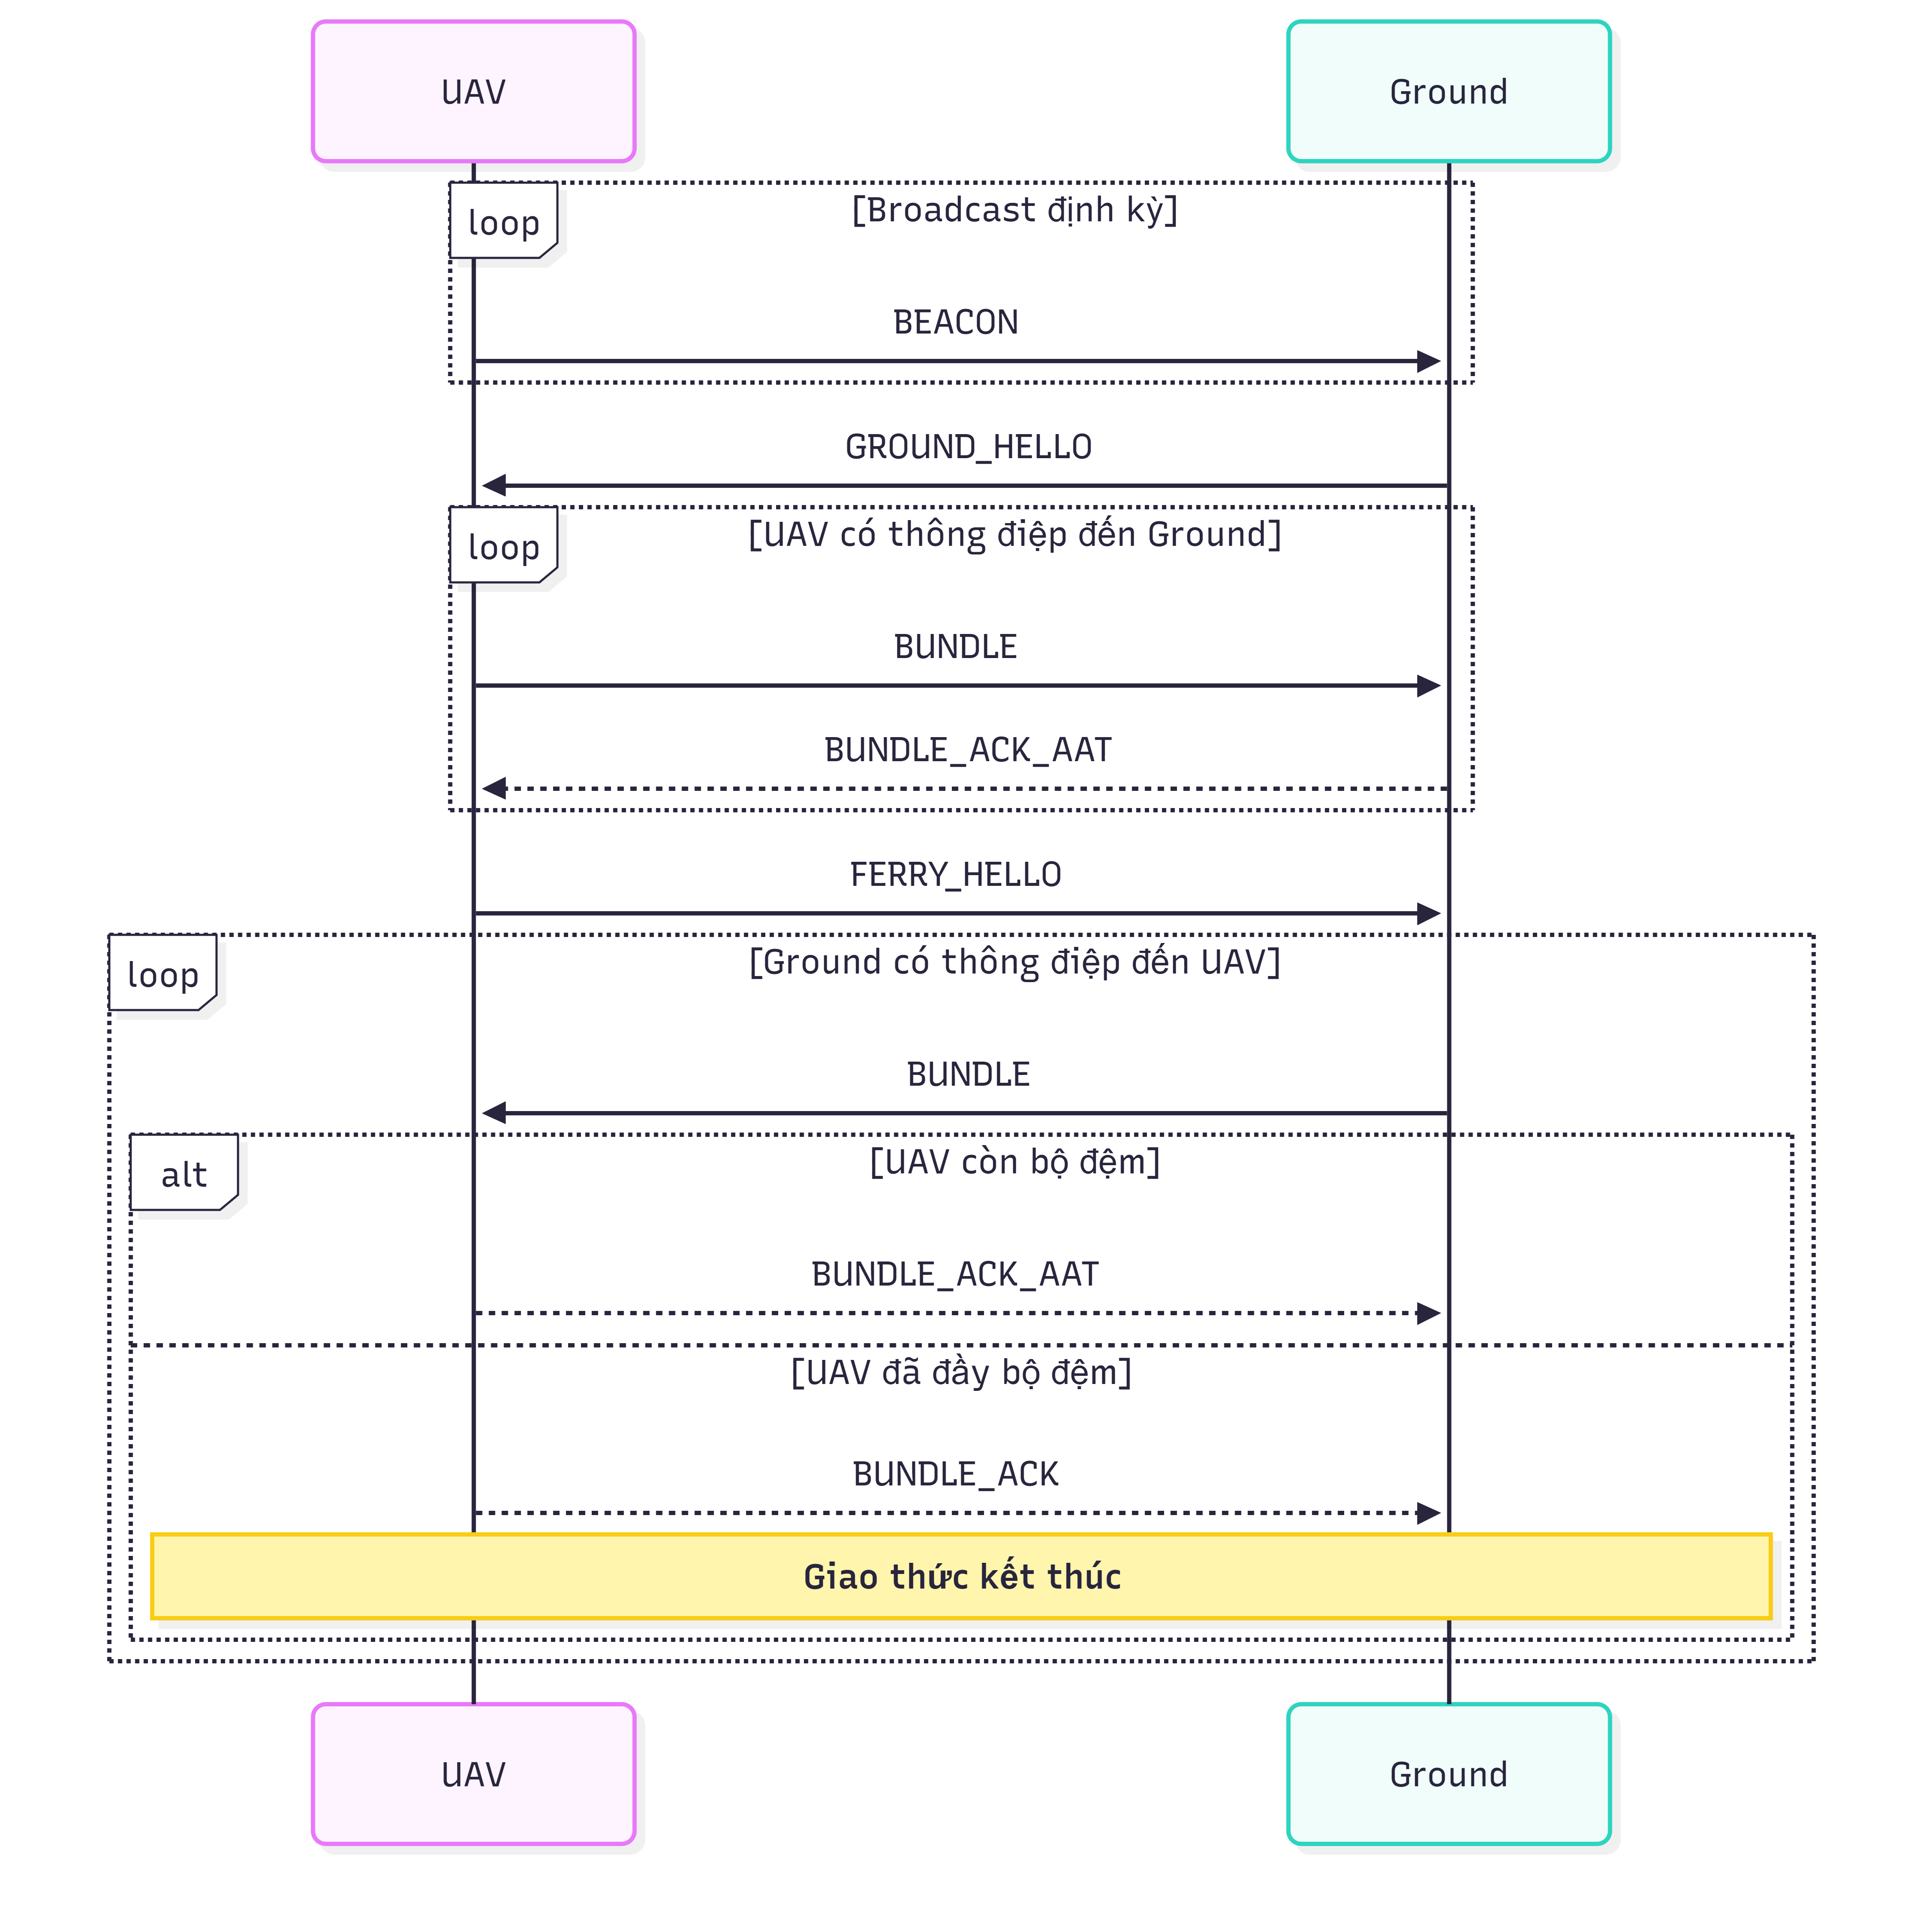
\includegraphics[width=0.5\textwidth]{image/ferry_to_ground.png}
  \caption{Quy trình thức trao đổi giữa nút mặt đất và UAV}
  \label{fig:ferry_to_ground}
\end{figure}

\subsubsection{Giao thức trao đổi giữa 2 UAV}

Khác với trao đổi giữa UAV và nút mặt đất, khi hai UAV trao đổi với nhau, chúng cần phải xét đến bộ đệm của từng UAV, một UAV không thể liên tiếp gửi các thông điệp vì bên nhận có thể bị tràn bộ đệm. Bên cạnh đó, trong thực tế do mỗi thông điệp (bundle) có kích thước lớn và thời gian truyền đáng kể, giao thức cần hạn chế xung đột bằng việc đảm bảo tại mỗi thời điểm chỉ có tối đa một thông điệp được truyền.

Để đảm bảo 2 uav có khả năng truyền thông điệp mà không cần lo lắng việc tràn bộ đệm, giao thức áp dụng cơ chế gửi luân phiên: hai uav thể luân phiên gửi thông điệp cho nhau, mỗi khi nhận được thông điệp, UAV gửi trả về ack để xác nhận và khiến cho UAV đối tác giải phóng bộ đệm, khi này UAV hiện tại có thể gửi một thông điệp mới. Với cách này, kể cả khi cả hai UAV chỉ có một vị trí trống trong bộ đệm thì chúng vẫn có thể trao đổi vô số thông điệp với nhau. Tại một thời điểm trong quá trình trao đổi, có nhiều nhất một nút giữ quyền gửi (tạm gọi là Token Owner), nút này sẽ gửi thông điệp đồng thời giao quyền gửi (Token) cho đối tác.
Giao thức trao đổi được chia làm 2 pha: Thiết lập nút giữ quyền gửi trước và trao đổi. Cụ thể:

\paragraph{Bắt tay: Thiết lập nút có quyền gửi trước}
\begin{itemize}
  \item Tương tự như khi trao đổi với nút mặt đất, các UAV liên tục broadcast các gói BEACON để tìm nút lân cận. Một UAV khi nhận BEACON, sẽ kiểm tra địa chỉ Ip của nút gửi và kiểm tra xem hiện hai UAV có đang trao đổi với nhau hay không.
  \item Nếu hai UAV đang không trao đổi, UAV có Ip thấp hơn sẽ phản hồi bằng gói FERRY-HELLO. UAV còn lại khi nhận FERRY-HELLO cũng sẽ phản hồi bằng FERRY-HELLO. Tại thời điểm này, một phiên trao đổi mới được thiết lập giữa hai UAV.
  \item Sau khi nhận FERRY-HELLO, UAV có Ip thấp hơn tạm thời giữ quyền gửi, UAV này sẽ kiểm tra bộ đệm của UAV đối tác (thông tin này được đính kèm trong gói FERRY-HELLO)
  \begin{itemize}
    \item Nếu bộ đệm của cả hai UAV đã đầy, giao thức sẽ kết thúc ngay lập tức.
    \item Nếu bộ đệm của UAV đối tác đầy và token owner có thể chứa thêm các thông điệp mới, nó sẽ gửi gói ACCEPT-TRANSFER để trao quyền gửi cho đối tác.
    \item Trường hợp còn lại, nó sẽ giữ quyền gửi.
  \end{itemize}
  \item Sau pha bắt tay này, hai UAV chuyển qua pha trao đổi
\end{itemize}

\paragraph{Trao đổi thông điệp và quyền gửi}
\begin{itemize}
  \item Nút giữ quyền gửi (Token owner) lựa chọn trong bộ đệm của mình một thông điệp cần gửi cho đối tác rồi gửi qua gói BUNDLE. Gói BUNDLE ngoài dữ liệu, nó còn mang ý nghĩa trao quyền gửi (Token) của mình cho đối tác.
  \item UAV nhận được BUNDLE sẽ kiểm tra:
  \begin{itemize}
    \item Nếu có thông điệp cần gửi, nó trở thành Token owner mới, trả về BUNDLE-ACK để UAV đối tác giải phóng bộ đệm, sau một khoảng thời gian ngắn, nó sẽ lặp lại bước đầu tiên để gửi thông điệp mới.
    \item Nếu không có thông điệp cần gửi, nó sẽ trả về BUNDLE-ACK hoặc BUNDLE-ACK-ATT dựa trên việc bộ đệm của nó đã đầy hay chưa. Gói BUNDLE-ACK-ATT ngoài việc xác nhận gói tin đã được nhận thành công, cũng mang ý nghĩa trao trả lại token để đối tác có thể gửi các thông điệp mới.
  \end{itemize}
  \item Giao thức sẽ kết thúc khi Token owner mói không được thiết lập, hoặc Token owner không có thông điệp nào để gửi hoặc bất kì gói tin nào trong quá trình trao đổi bị mất.
\end{itemize}

\begin{figure}
    \centering
    \subfloat[\centering Bắt tay]{{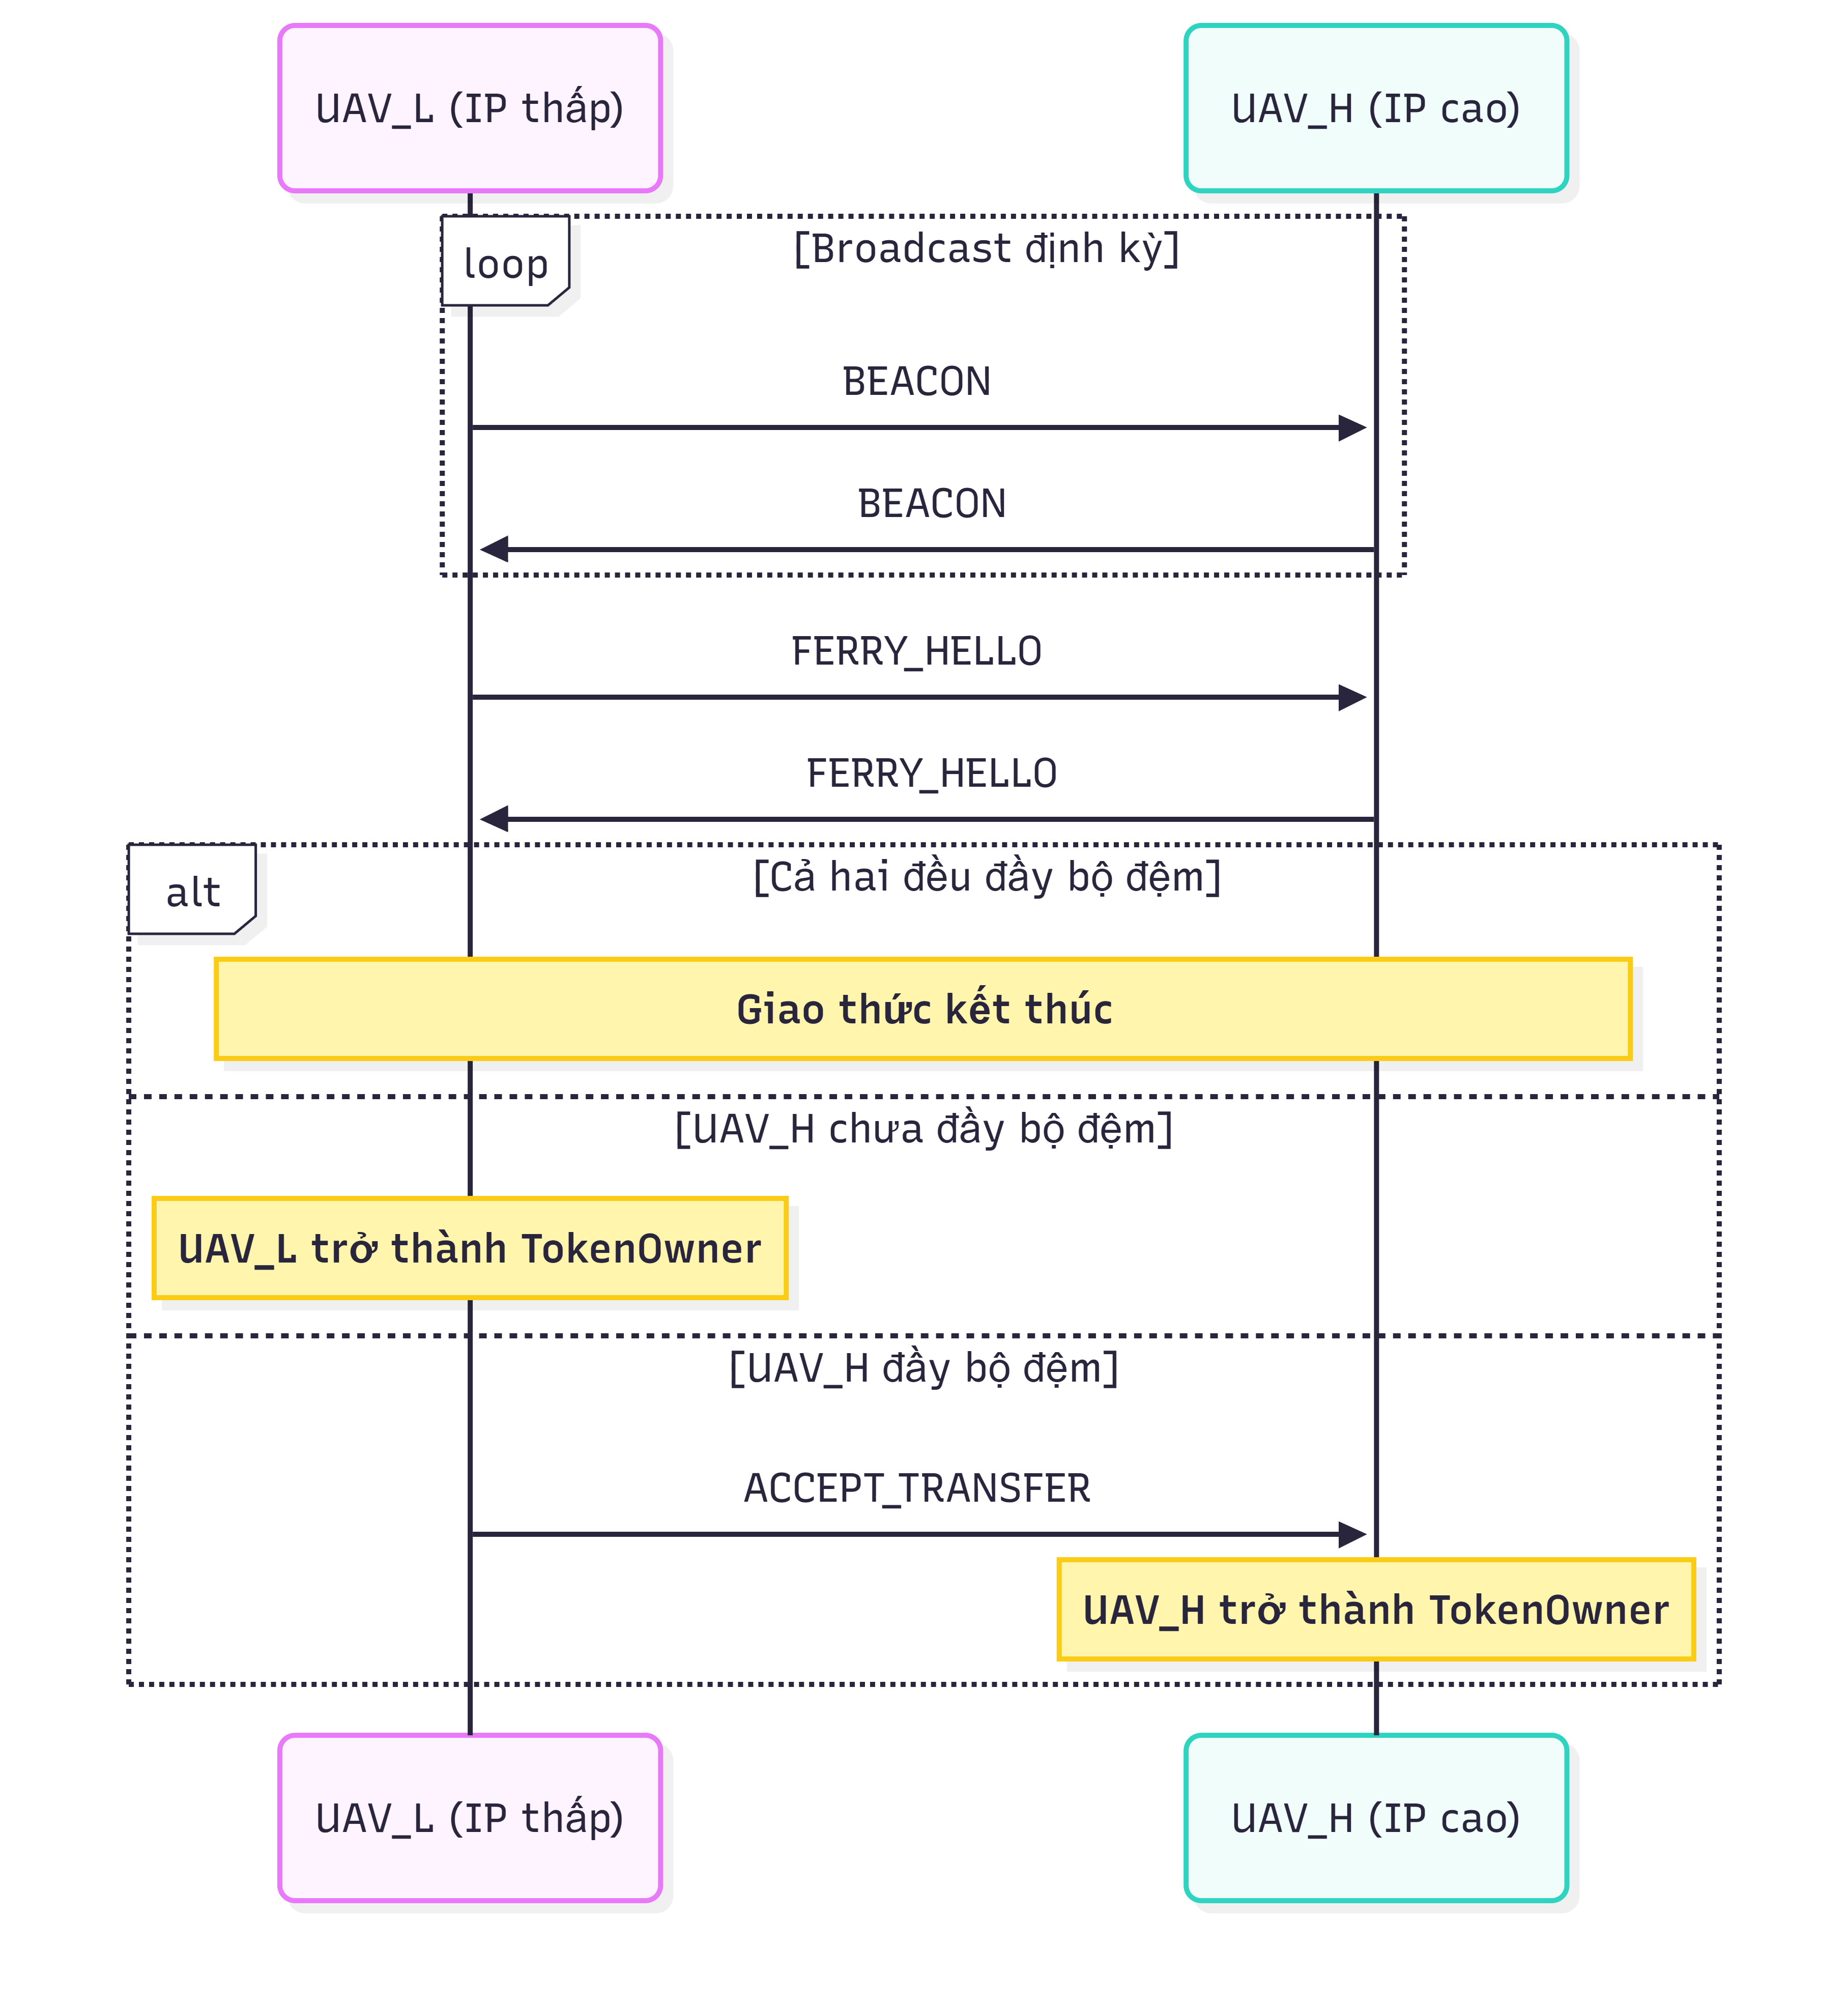
\includegraphics[width=0.46\textwidth]{image/ferry_to_ferry_1.png} }}%
    \qquad
    \subfloat[\centering Trao đổi]{{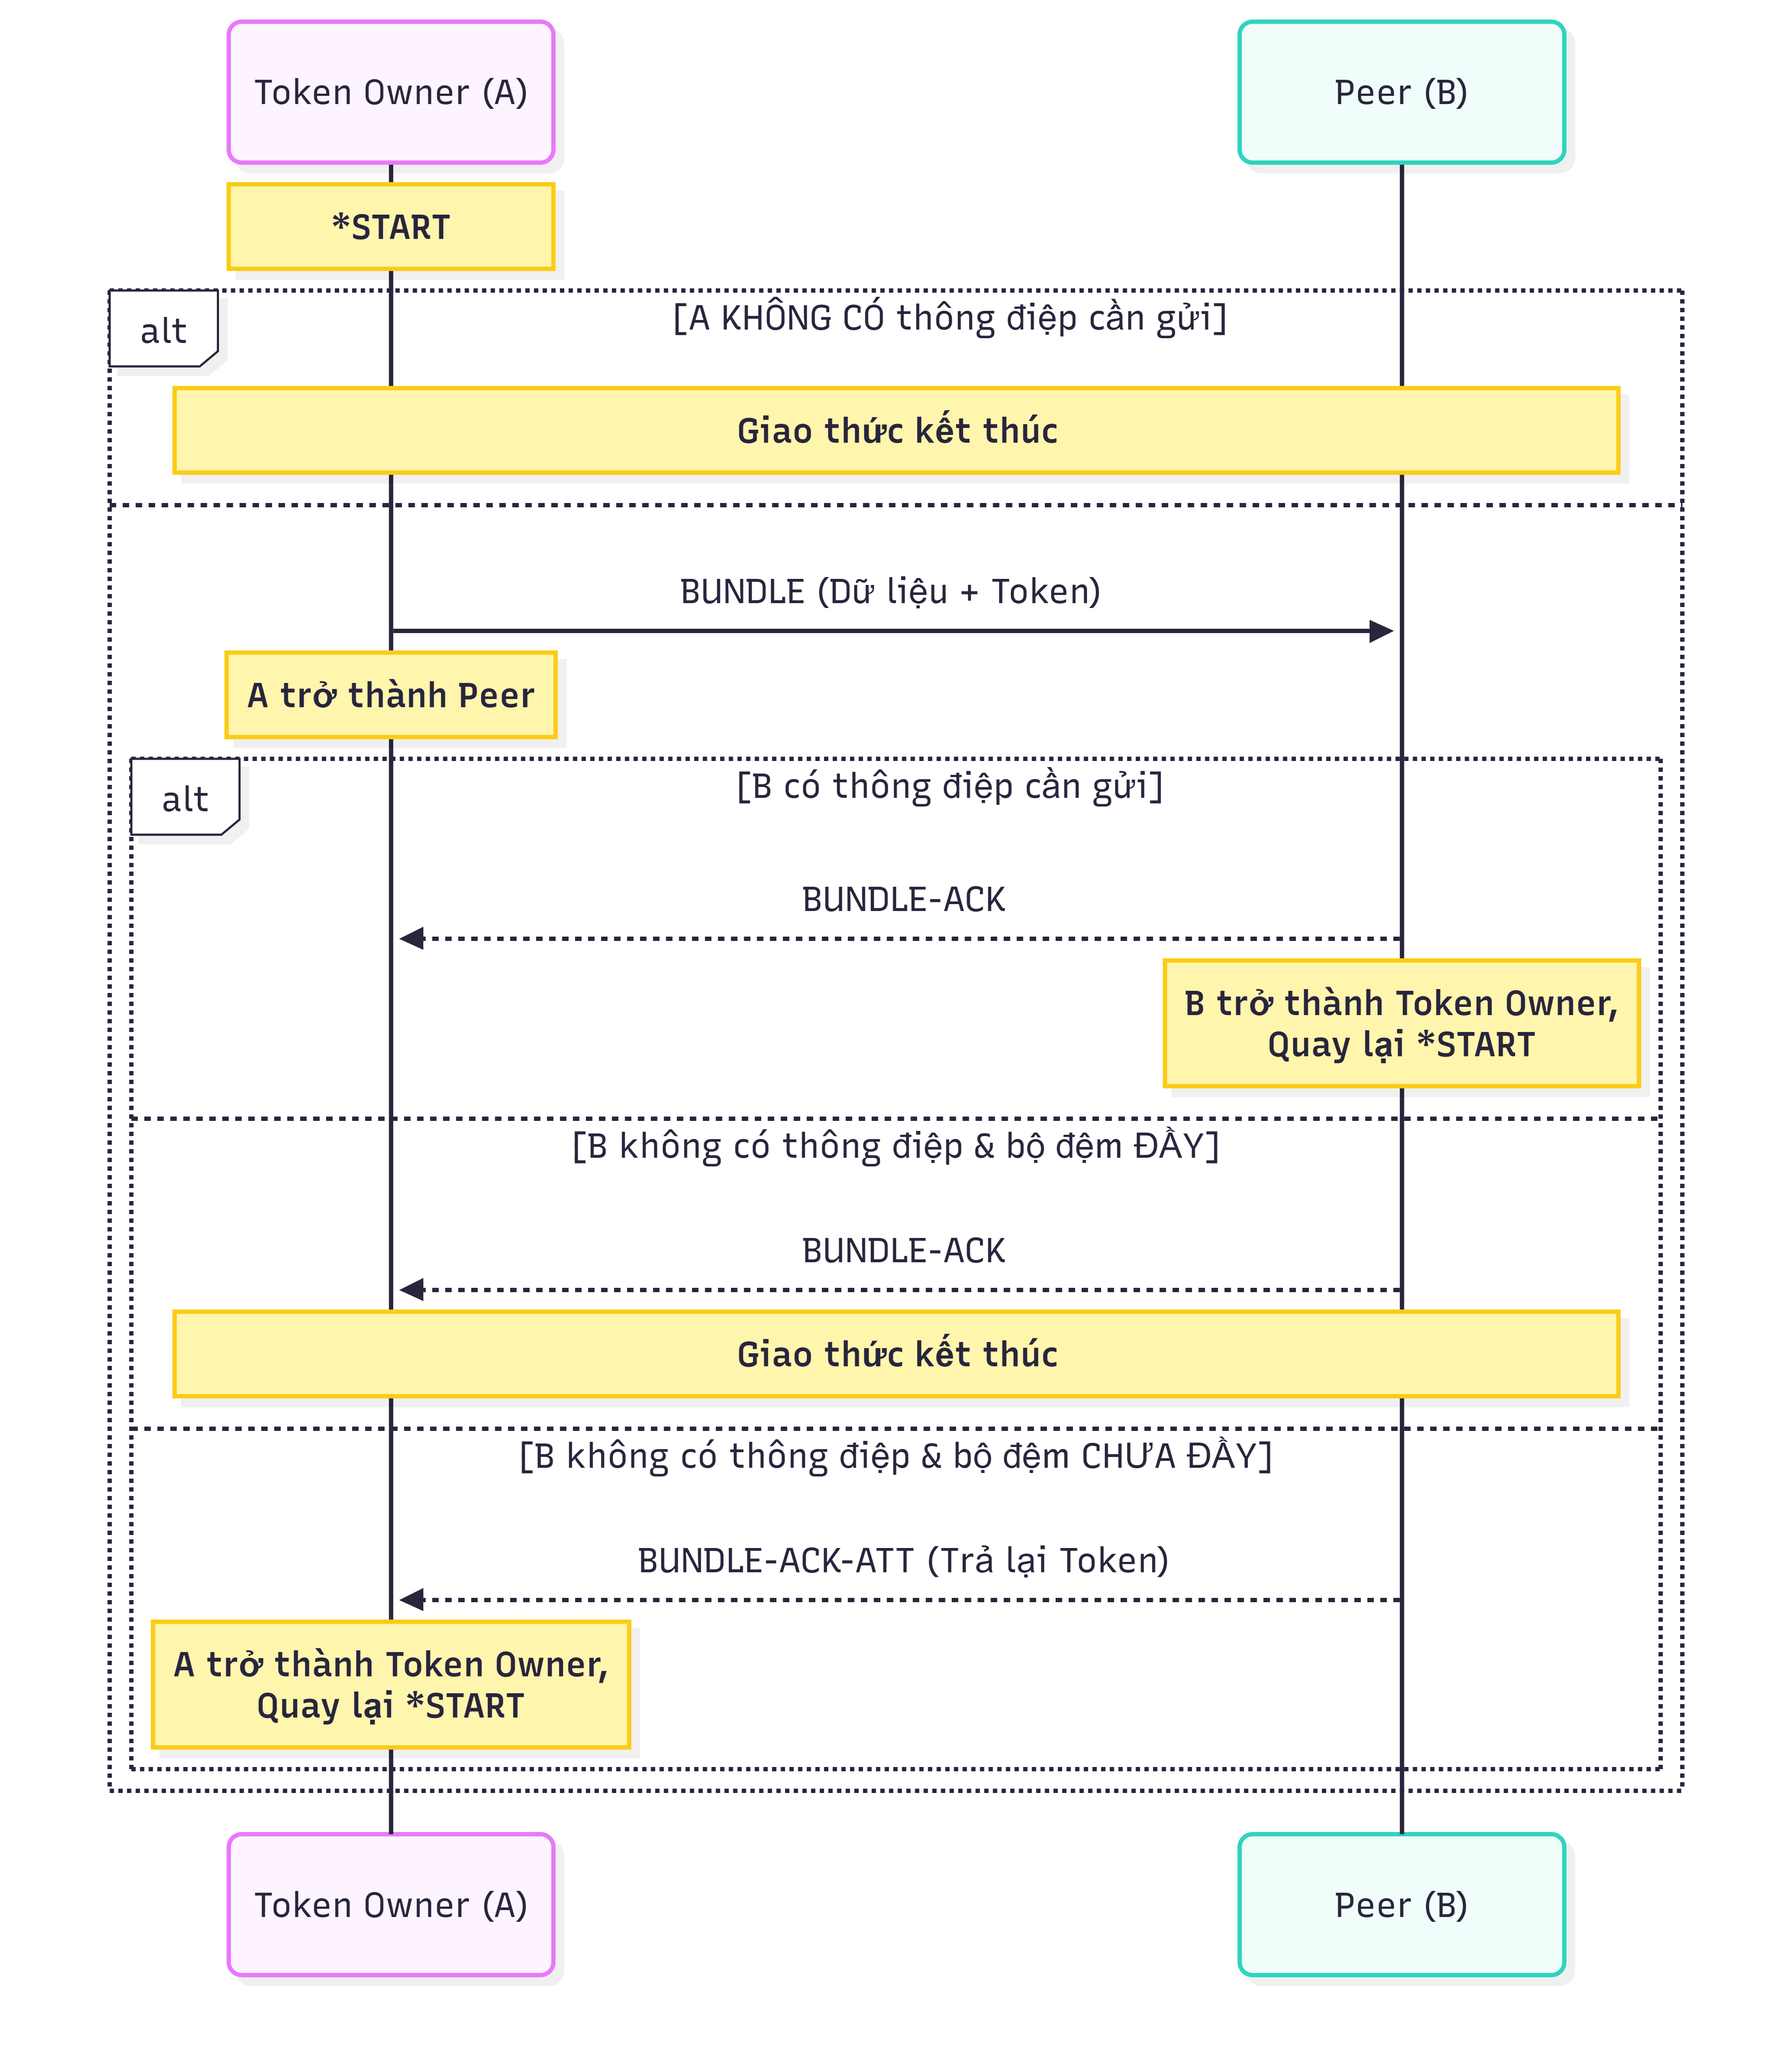
\includegraphics[width=0.46\textwidth]{image/ferry_to_ferry_2.png} }}%
    \caption{Quy trình bắt tay (a) và trao đổi (b) trong giao thức trao đổi giữa 2 UAV}%
    \label{fig:ferry_to_ferry}%
\end{figure}

\subsection{Thuật toán quy hoạch lộ trình 2 pha, định tuyến thông điệp và lập lịch di chuyển VH-mTSP-RE (Virtual Hub m-Traveling Saleman Problem and Route Extend)}
\subsubsection{Ý tưởng của thuật toán}
Các phương pháp quy hoạch lộ trình trước đó, Tabaf, DTP-TSP-D hay FPOD đều hoạt động theo cơ hội, các UAV ra quyết định nút nào để đi chuyển đến tiếp theo dựa trên quan sát đơn lẻ của chúng trong môi trường hiện tại. Các phương pháp này đều bộc lộ hai điểu yếu chính:
\begin{itemize}
  \item Thứ nhất là sự không công bằng, khi một cặp nút ở xa nhau, các thông điệp giữa chúng có thể bị bỏ qua vì các uav có thể chuyển nhiều thông điệp đến các nút ở gần uav hơn. Điều này khiến các thuật toán này khó tối thiểu hóa chỉ số dead connection và low connection.
  \item Thứ hai là sự thiếu hợp tác giữa các UAV, các lộ trình của một UAV phần lớn chỉ dựa trên quan sát của riêng UAV đó, điều này khiến cho dù khi số lượng UAV tăng, hiệu năng của các phương pháp này chỉ tăng rất chậm, thể hiện rõ ở phần thực nghiệm.
\end{itemize}

Để đạt được sự công bằng và giảm chỉ số dead connection và low connection về không, các uav phải coi việc phục vụ các nút ở xa nhau và gần nhau là như nhau. Việc này dẫn đến ý tưởng về một điểm trung chuyển, thay vì những người đưa thư cố di chuyển để gửi gói tin đến các vị trí ở gần mình, họ chuyển thư về một kho tổng, và nhiệm vụ chuyển thư đến đích sẽ do người đưa thư khác phù hợp hơn thực hiện. Ý tưởng này thể hiện sự công bằng giữa tất cả các nút trong mạng:
\begin{itemize}
  \item Khi hai nút ở xa nhau cần chuyền thông điệp, quãng đường mà thông điệp phải đi sẽ gần như là đường thẳng, giúp thông điệp đến đích kịp thời hạn.
  \item Khi hai nút ở gần nhau, thông điệp giữa chúng vẫn có thể phải đi qua điểm trung chuyển. Quãng đường mà thông điệp đi dài hơn, nhưng cũng không quá dài để thông điệp đến đích kịp thời.
\end{itemize}

Từ đây, ý tưởng trở thành việc các uav chia nhau đi để thu thập thông điệp, trao đổi với nhau tại một điểm trung chuyển (hub) rồi lại chia nhau đi để truyền thông điệp đến đích và thu thập thông điệp mới. VH-mTSP-RE sử dụng các thuật toán tối ưu hóa và các heuristic để thực hiện việc này qua hai pha chính: 
\begin{itemize}
  \item Pha 1: Hub mTSP: Các nút mặt đất được phân thành m nhóm ứng với từng UAV. Đồng thời ở bước này, một điểm trung chuyển tối ưu được tìm để các UAV sau khi thu thập thông điệp sẽ trao đổi với nhau, với kì vọng rằng quãng đường mà một thông điệp phải đi dài nhất là ngắn nhất và các UAV chia sẻ việc phục vụ các nút mặt đất với nhau một cách công bằng.
  \item Pha 2: Route Extend: Ở pha này, các UAV tận dụng thời gian còn lại sau khi hoàn thành nhiệm vụ của bản thân để đi đến các điểm khác, hỗ trợ việc thu thập thông điệp.
  \item Cuối cùng từ hai pha trên, một bảng định tuyến được xây dựng và các uav thực hiện việc đồng bộ lịch trình di chuyển theo chiến lược trung chuyển ảo (Virtual Hub): Các uav sẽ đợi nhau ở điểm trung chuyển, trao đổi với nhau, sau đó đi một vòng lộ trình và quay trở lại điểm trung chuyển và lặp lại.
\end{itemize}

\subsubsection{Pha 1: Hub mTSP} 
Pha 1 của VH-mTSP-RE, tạm gọi là bài toán H-mTSP, gần tương tự như việc giải bài toán mTSP, m người đưa thư phải chia nhau đi qua các vị trí để lấy và gửi thư, và thay vì có một điểm xuất phát (depot cho trước) như mTSP, ở bài toán H-mTSP, ta cần tự tìm một depot, một điểm trung chuyển tối ưu mà tất cả các người đưa thư đều phải ghé thăm. Lời giải cho bài toán H-mTSP cũng tương tự như bài toán mTSP, là một danh sách các lộ trình, ứng với việc từng uav sẽ phải ghé thăm các nút mặt đất nào, theo thứ tự ra sao. Bài toán H-mTSP có thể được phát biểu như sau: 

Cho một tập $n$ điểm \( P = \{p_1, p_2, \dots, p_n\} \subset \mathbb{R}^2 \), trong đó mỗi điểm biểu diễn một vị trí cần được phục vụ. Khoảng cách giữa hai điểm \( p_i, p_j \in P \) là $d(p_i, p_j)$, là khoảng cách Euclid giữa hai điểm trên mặt phẳng 2D.

Cho biết số lượng UAV là \( m \). Không giống như bài toán mTSP cổ điển, bài toán này yêu cầu đồng thời xác định một điểm trung chuyển (hub) \( h \in \mathbb{R}^2 \), không nhất thiết trùng với bất kì điểm nào trong \( P \).

Mỗi người UAV \( k \in \{1, \dots, m\} \) thực hiện một lộ trình khép kín bắt đầu từ trung chuyển \( h \), đi qua một tập con các điểm trong \( P \), và quay trở lại \( h \). Các hành trình này phải thỏa mãn các điều kiện sau:

\begin{itemize}
    \item Mỗi điểm \( p_i \in P \) được thăm đúng một lần bởi đúng một UAV.
    \item Mỗi hành trình bắt đầu và kết thúc tại hub \( h \).
    \item Các tập điểm được phân công cho các UAV là đôi một rời nhau và hợp của tât cả bằng \( P \).
\end{itemize}

Gọi \( R_k = (h, p_{k,1}, p_{k,2}, \dots, p_{k,\ell_k}, h) \) là lộ trình của UAV thứ \( k \). Khi đó, chi phí hay độ dài của lộ trình này được xác định bởi:
\begin{equation}
l_k(h) = d(h, p_{k,1}) + \sum_{i=1}^{\ell_k - 1} d(p_{k,i}, p_{k,i+1}) + d(p_{k,\ell_k}, h) + (\ell_k + 1) \times V_{uav} \times t_{hover}
\label{eq:route_length}
\end{equation}

Trong đó:
\begin{itemize}
  \item $V_{uav}$ là vận tốc của uav.
  \item $t_{hover}$ là thời gian uav bay lơ lửng mỗi khi đến phục vụ tại một vị trí.
  \item $\ell_k$ là số nút mặt đất được UAV k phục vụ.
\end{itemize}

Mục tiêu của bài toán là đồng thời xác định vị trí hub \( h \) và tập \( m \) hành trình sao cho:
\begin{itemize}
  \item Lộ trình dài nhất là ngắn nhất.
  \item Các lộ trình có độ dài tương tự nhau, hay các uav phải chia sẻ trách nhiệm phục vụ cho nhau một cách công bằng.
\end{itemize}

Bài toán mTSP và các biến thể của nó đã được xuất hiện trên nhiều nghiên cứu, sử dụng nhiều phương pháp khác nhau để giải quyết. Một trong trong thuật toán tối ưu hóa phổ biến nhất được dùng để giải bài toán mTSP là thuật toán di truyền, và ta có thể khéo léo áp dụng thuật toán di truyền và tìm kiếm cục bộ để tìm một lời giải cận tối ưu cho bài toán H-mTSP.

\paragraph{Hàm chi phí: Mục tiêu tối ưu}

Dù sử dụng bất cứ thuật toán tối ưu hóa nào, trước hết ta đều cần phải xác định mục tiêu tối ưu, cụ thể hóa nó bằng một hàm chi phí để đánh giá độ tốt của một lời giải. Với mỗi lời giải của bài toán, ta đều có thể tính toán được độ dài các lộ trình bằng (\ref{eq:route_length}), và từ thông tin về độ dài lộ trình, chúng ta có thể tính được một hàm chi phí như sau:
\begin{equation}
Cost = max(l_i | 1\le i \le m) + \alpha \times \frac 1m\sum_{i=1}^{m} l_i + \beta \times CEP + ERP
\end{equation}

Hàm chi phí là tổng của 4 thành phần:
\begin{itemize}
  \item Độ dài của lộ trình dài nhất 
  \item Độ dài trung bình các lộ trình
  \item Cap Exceed Penalty (CEP) - Phạt vượt ngưỡng
  \item Empty Route Penalty (ERP) - Phạt các lộ trình rỗng
\end{itemize}

Thành phần thứ nhất của hàm chi phí là tiêu chí Makespan, phản ánh mục tiêu quan trọng nhất của bài toán H-mTSP, đó là tối ưu để lộ trình dài nhất là ngắn nhất, nhằm tối thiểu hóa thời gian của một vòng phục vụ của các uav.
Tuy nhiên nếu chỉ tối ưu theo tiêu chí này, thuật toán thuật toán có thể tạo ra các lộ trình không hiệu quả cho các UAV còn lại, tạo ra các lộ trình vòng vèo, không tối ưu nhưng vẫn đảm bảo ngắn hơn lộ trình dài nhất. Thuật toán phải xét thêm các tiêu chí phụ. 

Tiêu chí phụ thứ nhất là độ dài trung bình các lộ trình. Tiêu chí này giúp thuật toán chọn các giải pháp có tổng quãng đường di chuyển ngắn hơn, khiến các lộ trình sạch sẽ, gọn gàng hơn. Không những thế, tiêu chí này cũng góp phần tối ưu độ dài lộ trình dài nhất, trong khi lai tạo và đột biết, nhóm các nút tạo nên lộ trình dài nhất có thể thay đổi và nhóm mới này có thể đã được tối ưu từ trước nhờ tiêu chí độ dài trung bình.

Tiêu chí phụ thứ hai là Cap Exceed Penalty (CEP) hay phạt vượt ngưỡng. Tuy CEP chỉ là tiêu chí phụ nhưng nó là một thành phần quan trọng giúp phân chia công việc cho các uav một cách công bằng. Công thức cơ bản của CEP như sau:
\begin{equation}
CEP = \frac 1 {cec} \sum_{i=1}^{m} \max(0, l_i - cap)
\end{equation}
Trong đó:
\begin{itemize}
  \item $cap$ là ngưỡng cho trước
  \item $cec$ hay Cap Exceed Count là số lộ trình có độ dài vượt ngưỡng $cap$. Trong trường hợp không có lộ trình nào vượt ngưỡng, $cec = 1$.
\end{itemize}

Mục đích của CEP là ép các uav phải san sẻ nhiệm vụ của mình một cách công bằng hơn. Cụ thể, nó ép các uav có lộ trình ngắn hơn ngưỡng cap phải phục vụ thêm để giảm tải cho các uav có lộ trình dài.
Việc chọn một ngưỡng cap hợp lý rất quan trọng, nó quyết định sự thành công của chiến lược này. Nếu ngưỡng càng thấp, khi này, phần lớn các lộ trình của uav đều lớn hơn ngưỡng này, giá trị tổng CEP tiến về tổng độ dài lộ trình. Còn nếu ngưỡng quá cao, khi này, các lộ trình phần lớn đều ngắn hơn, khiên CEP tiến về 0. Cả hai trường hợp đều khiến CEP mất đi mục tiêu chính của nó.
Để xác định một giá trị ngưỡng hợp lý, hãy xét các trường hợp xấu nhất của chiến lược Virutal Hub (trung chuyển ảo).

Kịch bản 1, xét hai nút mặt đất và hai uav phục vụ chúng. Theo chiến lược trung chuyển ảo, sẽ di chuyển giữa nút của mình và điểm trung chuyển Dễ thấy rằng điểm trung chuyển sẽ nằm ở chính giữa hai nút mặt đất, và hai uav sẽ có lộ trình dài bằng nhau, tạm gọi là $L$. Trong trường hợp xấu nhất, ngay sau khi uav vừa rời khỏi nút mặt đất để đi đến điểm chung chuyển, thì nút mặt đất đó tạo ra thông điệp mới, thông điệp này sẽ phải chờ uav quay lại ($L$), sau đó sẽ phải chờ trong bộ đệm của uav đến điểm chung chuyển ($\frac L2$), và chờ tiếp khi đi từ trung chuyển đến đích ($\frac L2$). Tổng thời gian mà gói tin phải chờ tương đương với thời gian mà uav đi một quãng đường có độ dài $2L$. Vậy nếu ta muốn đảm bảo tỉ lệ truyền thông điệp thành công là 100\%, thì với giới hạn Time-to-Live của thông điệp, độ dài lộ trình dài nhất của các uav phải nhỏ hơn: 
\begin{equation}
expectedMaxLength = \frac 1 2 \times TTL \times V_{uav}
\end{equation}

Trong đó $V_{uav}$ là vận tốc của uav.

Kịch bản 2, vẫn là hai uav nhưng chúng phải phục vụ nhiều nút hơn, tuy nhiên, ta chỉ cần quan tâm đến nút biên: nút A nằm ở đầu lộ trình của uav 1 và nút B nằm ở cuối lộ trình uav 2.
Trường hợp xấu nhất của kịch bản này, là ngay sau khi uav vừa rời khỏi nút A để đi đến điểm chung chuyển, thì nút A tạo ra thông điệp mới gửi đến B, thông điệp này sẽ phải chờ uav quay lại ($L$), sau đó sẽ phải chờ trong bộ đệm của uav đến điểm chung chuyển ($L - d(hub,A)$), và chờ tiếp khi đi từ trung chuyển đến đích ($L-d(hub,B)$). Tổng thời gian mà gói tin phải chờ tương đương với thời gian mà uav đi một quãng đường có độ dài tương đương $3L$. Tương tự, nếu ta muốn đảm bảo tỉ lệ truyền thông điệp thành công là 100\%, độ dài lộ trình dài nhất của các uav phải nhỏ hơn: 
\begin{equation}
expectedMaxLength \approx \frac 1 3 \times TTL \times V_{uav}
\end{equation}

Từ phân tích trên, ta có thể chọn hai ngưỡng mục tiêu hợp lý để thuật toán tìm được các lộ trình với độ dài phù hợp, đồng thời tránh sự phụ thuộc vào một ngưỡng cố định:
\begin{equation}
cap1 = \frac 1 3 \times TTL \times V_{uav}
\end{equation}
\begin{equation}
cap2 = \frac 1 2 \times TTL \times V_{uav}
\end{equation}

Khi này công thức CEP trở thành
\begin{equation}
CEP = \frac 1 {cec_1} \sum_{i=1}^{m} \max(0, l_i - cap1) + \frac 1 {cec_2} \sum_{i=1}^{m} \max(0, l_i - cap2)
\end{equation}

Trong trường hợp TTL đủ lớn, khiến giá trị $CEP = 0$. Khi này yêu cầu cân bằng chặt chẽ cũng không cần thiết nữa, do $\max l_i$ đã nhỏ hơn $expectedMaxLength$, các UAV luôn có thể phục vụ trong các trường hợp xấu nhất như đã phân tích. Còn nếu TTL quá nhỏ, ta chỉ còn cách chấp nhận hệ thống rất khỏ để có thể hoạt động tốt trong điều kiện đề ra.

Tiêu chí phụ cuối cùng là Empty Route Penalty (ERP). Đây chỉ là tiêu chí đơn giản giúp phạt các lời giải tạo ra các lộ trình rỗng. Tiêu chí này chỉ là phòng ngừa và việc tránh tạo ra lộ trình rỗng có thể được giải quyết ở các bước lai tạo và đột biến để tạo ra lời giải mới.

\begin{equation}
ERP = ERC \times penalty
\end{equation}
Trong đó:
\begin{itemize}
  \item ERC: Empty Route Count - Số lộ trình rỗng
  \item $penalty=2000$: mức phạt
\end{itemize}

Cuối cùng, sau khi thử nghiệm các trọng số, hai hàm chi phí sau được lựa chọn để sử dụng:
\begin{itemize}
  \item Hàm chi phí 1 cân bằng giữa việc tìm kiếm vùng nghiệm tốt và tối ưu theo mục tiêu makespan, hàm này được sử dụng trong quá trình tối ưu bằng thuật toán di truyền.
  \begin{equation}
    Cost_1 = max(l_i | 1\le i \le m) + 0.01 \times \frac 1m\sum_{i=1}^{m} l_i + 0.05 \times CEP + ERP
  \end{equation}
  \item Hàm chi phí 2 tập trung vào mục tiêu chính makespan, các tiêu chí phụ thì chỉ cải thiện nếu có thể, do vậy hàm này được sử dụng trong quá trình tinh chỉnh bằng tìm kiếm cục bộ:
  \begin{equation}
    Cost_2 = max(l_i | 1\le i \le m) + 0.001 \times \frac 1m\sum_{i=1}^{m} l_i + 0.005 \times CEP + ERP
  \end{equation}
\end{itemize}

\paragraph{Tìm điểm trung chuyển:}

Điểm trung chuyển tối ưu là một điểm sao cho lộ trình của một UAV (xuất phát từ trung chuyển, đi qua các nút nó cần phục vụ rồi qua lại) dài nhất là ngắn nhất. Từ một lời giải của bài toán, ta có thể tìm vị trí của điểm trung chuyển bằng một phương pháp tương tự như gradient descent trong học máy.

Đầu tiên, ta khởi tạo vị trí điểm trung chuyển ban đầu là trung tâm của các vị trí nút mặt đất, sau đó lặp lại thuật toán \ref{alg:hub} để tinh chỉnh: Đầu tiên, ta chèn vị trí chung chuyển vào từng lộ trình (trước điểm đầu, sau điểm cuối), sau đó tìm lộ trình dài nhất và kéo vị trí điểm trung chuyển về gần các nút trong lộ trình đó. Sau khi lặp lại việc tinh chỉnh với learning rate giảm dần, chúng ta sẽ có được một điểm hub tối ưu sau cho lộ trình dài nhất là ngắn nhất. Đồng thời đảm bảo rằng 2 hoặc 3 lộ trình dài nhất dài tương đương nhau. Điểm trung chuyển cuối cùng này sẽ được chèn vào các lộ trình để tính hàm chi phí theo công thức đã đề cập ở mục trước.

\begin{algorithm}
\caption{Tinh chỉnh vị trí hub}
\label{alg:hub}
\begin{algorithmic}[1]

\Require Vị trí ban đầu $h$, danh sách lộ trình (không chứa hub) $\{R_1,\dots,R_m\}$, số vòng lặp $T$, learning rate $\alpha$
\Ensure Vị trí sau tinh chỉnh $h$

\While{$T > 0$}
    \State $T \gets T - 1$

    \For{mỗi uav $i$}
        \State $R'_i \gets$ Chèn hub $h$ vào lộ trình $R_i$
        \State Tính độ dài $l'_i$
    \EndFor

    \State $k \gets \arg\max_i l;_i$

    \State $p \gets$ chọn ngẫu nhiên điểm đầu hoặc điểm cuối của $R_k$

    \State $h \gets (1-\alpha) \times h + \alpha \times p$
\EndWhile

\State \Return $h$

\end{algorithmic}
\end{algorithm}

\paragraph{Chromosome: Biểu diễn lời giải}

Sau khi có được cách tính điểm trung chuyển và hàm chi phí, ta có thể đi sâu vào các kỹ thuật liên quan tới thuật toán di truyền, đầu tiên là thiết kế nhiễm sắc thể (chromosome). Lời giải của bài toán có thể được biểu diễn dưới dạng một nhiễm sắc thể gồm hai phần (Hình \ref{fig:twopart_chromosome}):
\begin{itemize}
  \item Phần 1 - Permuation: Một dãy số với độ dài $n$, là hoán vị thứ tự các nút mặt đất mà uav cần ghé thăm.
  \item Phần 2 - RouteLen: Một dãy số nguyên dương có độ dài $m$, thể hiện số lượng nút mặt đất mà từng uav sẽ phục vụ.
\end{itemize}

\begin{figure}
  \centering
  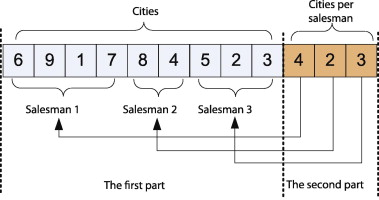
\includegraphics{image/twopart_chromosome.jpg}
  \caption{Biểu diễn nhiễm sắc thể}
  \label{fig:twopart_chromosome}
\end{figure}

Việc lai ghép và đột biến để tạo nhiễm sắc thể mới được thực hiện như sau:

\begin{itemize}
  \item Lai ghép: 
  \begin{itemize}
    \item Phần một của nhiễm sắc thể được lai ghép theo Ordered Crossover, một đoạn trong gene mẹ được chọn và giữ lại, đoạn sau được điền vào theo thứ tự xuất hiện trong gene cha.
    \item Phần hai của nghiễm sắc thể được lai ghép theo Single-Point Crossover, một điểm cắt được chọn, và phần trước điểm cắt sẽ được sao chép từ gene mẹ, phần sau điểm cắt sẽ được sao chép từ gene cha (hoặc ngược lại theo tỉ lệ 50-50). Sau đó, ta thực hiện thêm hoặc bớt một cách ngẫu nhiên để tổng của phần RouteLen bằng $n$.
  \end{itemize}
  \item Đột biến:
  \begin{itemize}
    \item Swap: Đổi trỗ hai vị trí ngẫu nhiên trong Permutation.
    \item Move: Di chuyển một điểm ngẫu nhiên trong một lộ trình ngẫu nhiên, sang một vị trí ngẫu nhiên của một lộ trình ngẫu nhiên khác.
    \item Reverse: Đảo ngược một đoạn ngẫu nhiên trong một lộ trình ngẫu nhiên.
  \end{itemize}
\end{itemize}

\paragraph{Các kỹ thuật di truyền được sử dụng}

Sau nhiều lần thử nghiệm và so sánh kết quả của các phiên bản thuật toán di truyền với bài toán H-mTSP, nhận thấy rằng thuật toán di truyền ban đầu có xu hướng hội tụ sớm và ít cải thiện ở các thế hệ sau, một số kỹ thuật đã được sử dụng để khắc phục vấn đề này:

\begin{itemize}
  \item \textbf{Elite-Rank based Roulette selection}: Ở mỗi lần lựa chọn lai tạo, hai cá thể được chọn ngẫu nhiên theo cơ chế xếp hạng (Rank-based Roulette), một cá thể sẽ được chọn trong nhóm tinh hoa (elite - 50\% cá thể tốt nhất), cá thể còn lại được chọn trên toàn bộ quần thể.
  \item \textbf{Giới hạn tuổi thọ}: Khi một cá thể tồn tại quá lâu, nó sẽ bị loại bỏ và thay thế bằng cá thể ngẫu nhiên mới. Tránh việc các nghiệm tối ưu cục bộ chi phối việc khám phá của thuật toán trong thời gian dài.
  \item \textbf{Reset Injection}: Tại một số mốc thế hệ định trước, 75\% cá thể tệ nhất sẽ bị loại bỏ và thay thế bằng các cá thể ngẫu nhiên. Giúp tái khởi động quá trình tìm kiếm của thuật toán.

\end{itemize}

\paragraph{Tìm kiếm cục bộ (local search): cải thiện kết quả tìm được}

Sau khi tìm được một lời giải tốt cho bài toán H-mTSP qua thuật toán di truyền, ta có thể chạy thêm một thuật toán tìm kiếm cục bộ tham lam để có thể cải thiện kết quả tìm được. Bước này sử dụng hàm chi phí $Cost_2$ đã đề cập ở phần trước.

Thuật toán \ref{alg:local_search_hmtsp} lặp lại việc thử các lân cận của lời giải tốt nhất tìm được: thử chuyển một nút từ uav này sang uav khác, hoặc hoán đổi hai nút giữa hai uav, và dừng lại khi không thấy cải thiện. Một lưu ý khi tính chi phí cho lời giải là khi thực hiện việc di chuyển nút giữa các uav thì thứ tự lộ trình ban đầu đã bị xáo trộn, vì vậy khi tính chi phí, khóa luận sử dụng heurisic 3-opt cho bài toán TSP để có được các lộ trình và vị trí chèn điểm trung chuyển vào lộ trình tối ưu. Thuật toán tinh chỉnh điểm trung chuyển cũng có thay đổi nhỏ, thay vì kéo về điểm đầu hoặc cuối lộ trình như thuật toán \ref{alg:hub}, điểm trung chuyển sẽ được kéo về một điểm ngẫu nhiên trên lộ trình dài nhất.

\begin{algorithm}
\caption{Local Search H-mTSP}
\label{alg:local_search_hmtsp}
\begin{algorithmic}[1]

\Require lời giải ban đầu $C = \{R_1, \dots, R_m\}$, số uav $m$
\Ensure Lời giải tối ưu cục bộ $C^*$

\State $C^* \gets C$
\State $bestCost \gets \text{Cost}(C^*)$

\State $improved \gets True$
\While{$improved$}
    \State $improved \gets False$
    \State $C^{**} \gets C^*$
    \Comment{Lưu lời giải tốt nhất tìm được trong vòng lặp này}

    \For{$i = 1$ to $m$}
        \Comment{--- MOVE: di chuyển một điểm sang uav khác ---}
        \For{$p \in C^*_i$}
            \For{$j = 1$ to $m$, $j \ne i$}
                \State $C' \gets C^*$
                \State Di chuyển $p$ từ $C'_i$ sang $C'_j$ 
                \State $newCost \gets \text{Cost}(C')$
                \If{$newCost < bestCost$}
                    \State $C^{**} \gets C'$
                    \State $bestCost \gets newCost$
                    \State $improved \gets true$
                \EndIf
            \EndFor
        \EndFor
    \EndFor

    \For{$i = 1$ to $m$}
        \Comment{--- SWAP: hoán đổi điểm giữa hai uav ---}
        \For{$j = i+1$ to $m$}
            \For{$p \in C^*_i$}
                \For{$q \in C^*_j$}
                    \State $C' \gets C^*$
                    \State Hoán đổi $p$ và $q$
                    \State $newCost \gets \text{Cost}(C')$
                    \If{$newCost < bestCost$}
                        \State $C^{**} \gets C'$
                        \State $bestCost \gets newCost$
                        \State $improved \gets true$
                    \EndIf
                \EndFor
            \EndFor
        \EndFor
    \EndFor
    \State $C^* \gets C^{**}$
\EndWhile

\State \Return $C^*$

\end{algorithmic}
\end{algorithm}

\subsubsection{Pha 2: Route Extend}

Từ phân tích ở phần trước, có thể thấy là để đảm bảo 100\% tỷ lệ truyền thông điệp thành công, thì độ dài của lộ trình dài nhất không được vượt quá $\frac 1 3 TTL \times V_{uav}$. 
Việc giải bài toán H-mTSP có thể tối thiểu hóa được lộ trình dài nhất, tuy nhiên nó không đảm bảo được độ dài lộ trình dài nhất không lớn hơn ngưỡng trên.
Việc này ảnh hưởng đến tỷ lệ truyền thành công của các nút, đặc biệt là những nút ở đầu và ở cuối lộ trình của các uav (tính từ điểm trung chuyến).

Trong trường hợp xấu: 
\begin{itemize}
  \item Với nút ở đầu lộ trình, uav vừa rời đi thì nút tạo thông điệp mới, thông điệp đó phải đợi một khoảng $l_{max}$ để uav quay lại và chờ trong bộ đệm một khoảng tương đương $l_{max}$ để được đưa đến điểm trung chuyển.
  \item Với nút ở cuối lộ trình uav, một thông điệp gửi đến nút đó phải chờ thêm một khoảng tương đương $l_{max}$ để được đưa từ điểm trung chuyển đến đích.
\end{itemize}

Nhận thấy rằng sau khi giải bài toán H-mTSP, một số uav có lộ trình ngắn hơn, và theo chiến lược trung chuyển ảo, những uav này sẽ phải chờ các uav khác tại điểm trung chuyển rồi mới có thể đi một vòng lộ trình của mình. 
Những uav này có thể tận dụng thời gian chờ có thể mở rộng lộ trình của mình để đi đến các nút ở đầu lộ trình, không chỉ của chính nó, mà có thể của các uav khác nữa, để hỗ trợ thu thập thêm các thông điệp mới được tạo tại các nút này.
Tuy nhiên các uav này vẫn phải đảm bảo truyền thông điệp đến các nút trong lộ trình ban đầu của bản thân kịp thời hạn, và chỉ nhận nhiệm vụ hỗ trợ thu thập tại các nút mới, nên các nút mới sẽ chỉ được thêm vào cuối lộ trình của một uav, sau khi chúng đã đi hết các nút cần phục vụ trong lộ trình ban đầu của mình và bên cạnh đó phải đảm bảo không làm tăng độ dài lộ trình vượt quá $l_{\max}$.
Ngoài ra, sau khi đi hết lộ trình ban đầu, thì thời gian để uav đến điểm trung chuyển là không nhiều, khi này nếu một nút được uav phục vụ, thì các thông điệp lấy được từ nút đó đều sẽ được chuyển đến trung chuyển rất nhanh, do vậy:
\begin{itemize}
  \item Một nút cần hỗ trợ thu thập là một nút ở đầu lộ trình của các uav tìm được qua pha H-mTSP, cụ thể hơn, khoảng cách theo lộ trình từ điểm trung chuyển đến nút này $< \frac 1 2 l_{max}$. Nút càng ở gần đầu lộ trình thì càng cần được ưu tiên.
  \item Một nút cần hỗ trợ thu thập chỉ cần được hỗ trợ bởi một uav.
\end{itemize}

Từ các kết luận trên, ta có thể phát biểu bài báo Route Extend như sau:

Cho $m$ lộ trình \( \{R_i\}_{k=1}^m \) (có được từ pha H-mTSP), trong đó mỗi lộ trình có dạng
$R_k = (h, p_{k,1}, p_{k,2}, \dots, p_{k,\ell_k}, h)$,
với $h \in \mathbb{R}^2$ là điểm trung chuyển đã được xác định trước. $l_k$ là độ dài của lộ trình $R_k$, và $l_{\max}$ là độ dài lộ trình dài nhất. Và $n'$ nút cần hỗ trợ $U = \{u_1, u_2, \dots, u_n'\} \subset P$, mỗi nút $u_i$ được gán một giá trị ưu tiên $priority(u_i) > 0$, ứng với mức độ quan trọng của việc hỗ trợ nút đó.

Mục tiêu của bài toán là mở rộng các lộ trình hiện có bằng cách chèn thêm một số nút từ $U$ vào cuối mỗi lộ trình (trước khi quay về hub), sao cho thu được các lộ trình mới, sao cho:
\begin{itemize}
  \item Mỗi nút $u_i \in U$ được chèn vào nhiều nhất một lộ trình.
  \item Độ dài của mỗi lộ trình mở rộng không vượt quá makespan ban đầu:

  $l'_k \leq l_{\max}, \quad \forall k = 1, \dots, m$
  \item Tổng mức độ hỗ trợ là lớn nhất:
\end{itemize}

Do bài toán có các ràng buộc mạnh, không phải nút nào cũng có thể hỗ trợ được, khiến việc tìm một thuật toán tối ưu hóa và biểu diễn lời giải thích hợp trở nên khó khăn. Để đơn giản hơn, ta có thể sử dụng thuật toán luyện kim cùng heurisic tham lam để ước lượng một lời giải tốt cho bài toán này.

\paragraph{Chuẩn bị}

Đầu tiên, ta chọn chiều di chuyển cho các uav. Trong hai chiều của lộ trình, ta chọn chiều có khoảng cách từ điểm trung chuyển đến nút đầu tiên là nhỏ hơn. Chiều di chuyển này giúp giảm thời gian một thông điệp phải chờ trong bộ đệm của UAV khi đi từ trung chuyển đến nút đích, đồng thời tạo ra nhiều cơ hội cho việc thêm nút vào lộ trình.

Sau đó, ta lọc ra các nút cần hỗ trợ, là các nút mà theo lộ trình hiện tại, khoảng cách từ điểm trung chuyển đến chúng, đi theo chiều đã xác định ở trên, nhỏ hơn nửa độ dài lộ trình dài nhất hay $d_{route}(hub,node) < \frac 1 2 l_{max}$. Nút càng gần điểm trung chuyển thì càng cần hỗ trợ:
\begin{equation}
priority(node) = \frac 1 2 l_{max} - d_{route}(hub,node)
\end{equation}
Giá trị này giúp các uav cố gắng hỗ trợ các nút cần được ưu tiên hơn, thay vì cố gắng hỗ trợ nhiều nút nhất có thể.

\paragraph{Chiến lược tham lam}

Một phương án chèn được biểu diễn bởi thứ tự xét các nút cần hỗ trợ. Với một thứ tự cho trước, ta thực hiện chèn tham lam như sau: với mỗi nút, tìm lộ trình đầu tiên có thể chèn nút đó vào cuối mà không vi phạm ràng buộc độ dài. Nếu tìm được, thực hiện chèn, ngược lại, bỏ qua nút đó. Độ tốt của phương án là tổng độ ưu tiên của các nút được chèn: Thuật toán \ref{alg:greedy_insertion}.

\begin{algorithm}
\caption{Chèn tham lam dưới ràng buộc độ dài}
\label{alg:greedy_insertion}
\begin{algorithmic}[1]

\Require Danh sách nút cần hỗ trợ $U$ (theo thứ tự), các lộ trình $R_1, \dots, R_m$, ngưỡng độ dài $L_{\max}$
\Ensure Tổng thưởng $Reward$, Các lộ trình mới $R'_1, \dots, R'_m$

\State $Reward \gets 0$

\For{$u \in U$}
    \For{$i = 1$ to $m$}
        \State $R'_i \gets R_i$
        \State Thêm $u$ vào cuối $R'_i$
        \State Tính độ dài mới $l'_i$

        \If{$l'_i \le L_{\max}$}
            \State $R_i \gets R'_i$
            \State $Reward \gets Reward + priority(u)$
            \State \textbf{break}
        \EndIf
    \EndFor
\EndFor

\State \Return $Reward$, $R'_1, \dots, R'_m$

\end{algorithmic}
\end{algorithm}

\paragraph{Sử dụng thuật toán luyện kim}

Không gian nghiệm của bài toán là tất cả các hoán vị của tập nút cần hỗ trợ $U \subset P$. 
Mỗi nghiệm tương ứng với một thứ tự chèn và có thể đánh giá độ tốt thông qua thuật toán chèn tham lam đã trình bày ở trên. Với mỗi nghiệm $X = (u_1, \dots, u_{n'})$, ta áp dụng thuật toán \ref{alg:greedy_insertion} để có được tổng thưởng $Reward(X)$. 
Giá trị này được chuẩn hóa:
\begin{equation}
\overline{Reward}(X) = \frac{Reward(X)}{\sum_{u \in U} priority(u)}.
\end{equation}

Hàm chi phí tương ứng là:
\begin{equation}
ReCost(X) = -\overline{Reward}(X).
\end{equation}

Nghiệm lân cận được tạo ra bằng việc đảo ngẫu nhiên một đoạn con trong hoán vị. Cụ thể, chọn ngẫu nhiên hai vị trí $i < j$ và đảo ngược thứ tự các phần tử trong đoạn $[i, j]$:
\[
(u_1, \dots, u_i, \dots, u_j, \dots, u_{n'})
\;\rightarrow\;
(u_1, \dots, u_j, \dots, u_i, \dots, u_{n'}).
\]

Thuật toán luyện kim được sử dụng để tìm kiếm một thứ tự chèn tốt hơn. Tại mỗi vòng lặp, một nghiệm lân cận được sinh ra và được chấp nhận theo tiêu chí xác suất phụ thuộc vào nhiệt độ: Thuật toán \ref{alg:sa_route_extend}

\begin{algorithm}
\caption{Simulated Annealing cho bài toán Route Extend}
\label{alg:sa_route_extend}
\begin{algorithmic}[1]

\Require Tập nút $U$, nhiệt độ ban đầu $T_0$, hệ số làm nguội $\alpha$, số vòng lặp $I$, hàm chi phí $Cost$
\Ensure Nghiệm tối ưu tìm được $X^*$

\State $X \gets RandomShuffle(U)$
\State $X^* \gets X$
\State $Cost^* \gets Cost(X)$
\State $T \gets T_0$

\For{$iter = 1$ to $I$}
    \State Sinh nghiệm lân cận $X'$
    \State $\Delta \gets Cost(X') - Cost(X)$

    \If{$\Delta < 0$}
        \State $X \gets X'$
    \Else
        \State $accept \gets true$ với xác suất $\exp(-\Delta / T)$
        \If{$accept == true$}
            \State $X \gets X'$
        \EndIf
    \EndIf

    \If{$ReCost(X) < Cost^*$}
        \State $X^* \gets X$
        \State $Cost^* \gets ReCost(X)$
    \EndIf

    \State $T \gets \alpha \cdot T$
\EndFor

\State \Return $X^*$

\end{algorithmic}
\end{algorithm}

\begin{figure}%
    \centering
    \subfloat[\centering Hub mTSP]{{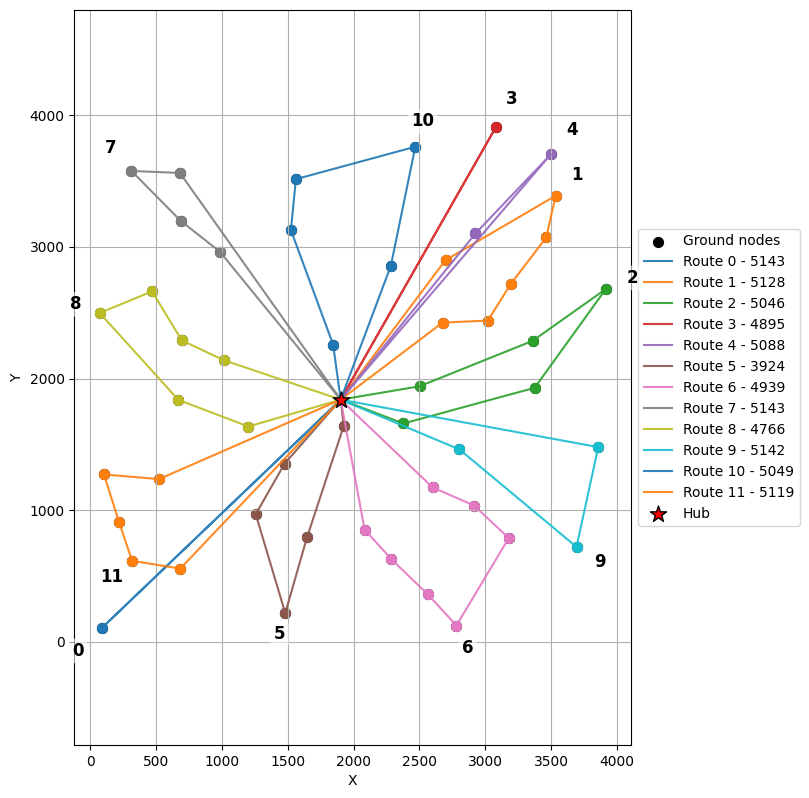
\includegraphics[width=0.45\textwidth]{image/pathplan_1.png} }}%
    \qquad
    \subfloat[\centering Route Extend]{{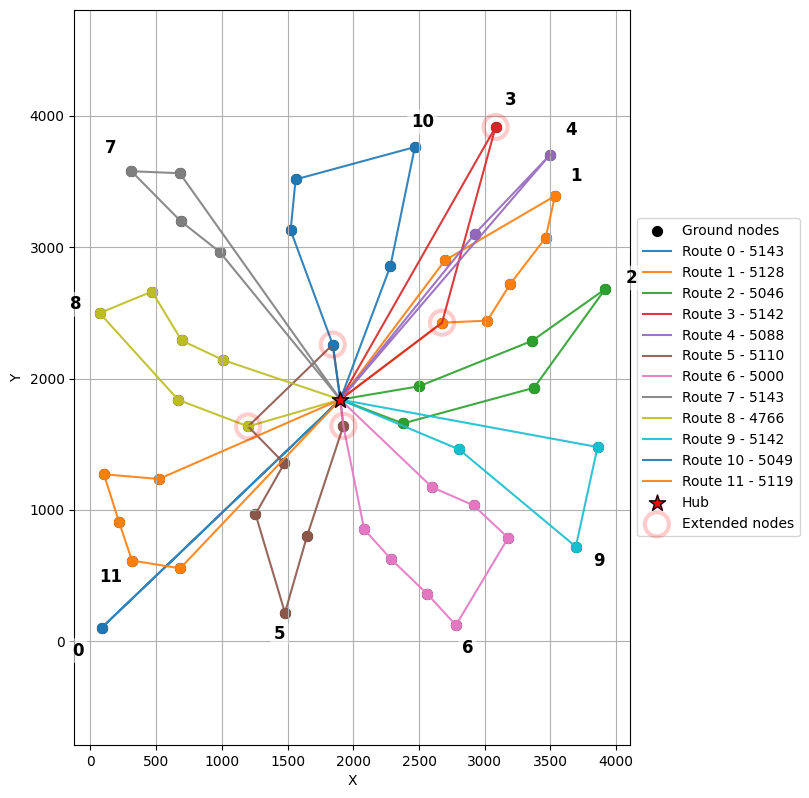
\includegraphics[width=0.45\textwidth]{image/pathplan_2.png} }}%
    \caption{Lộ trình tìm được qua 2 pha của thuật toán}%
    \label{fig:example}%
\end{figure}

\subsubsection{Lập lịch di chuyển của các UAV}

Đề xuất quan trọng của đề tài là chiến lược {\bfseries điểm trung chuyển ảo}: thay vì sử dụng một UAV đứng yên làm trung chuyển, các UAV sẽ đợi nhau ở điểm trung chuyển, trao đổi rồi mới phân tản ra để truyền các thông điệp đến đích, đồng thời thu thập các thông điệp mới. 

Nhưng tại sao lại phải như vậy ? Hãy xét các trường hợp tốt nhất và xấu nhất của hai chiến lược trung chuyển ảo và thực, với giả thiết lộ trình các UAV được chia sẻ cân bằng với độ dài $L$.
Ta xét nút A là nút tạo thông điệp, ở đầu lộ trình của UAV 1, nút B là đích đến của thông điệp được tạo, ở cuối lộ trình của UAV 2. 

Dễ thấy trường hợp tốt nhất của cả hai chiến lược đều là khi UAV 1 vừa đến thì nút A tạo thông điệp mới, và UAV 1 đến điểm trung chuyển thì UAV 2 cũng có mặt ở đó. Thông điệp sẽ phải chờ một khoảng tương đương $L$ để từ A đến trung chuyển và thêm một khoảng $L$ nữa để từ trung chuyển đến B.

Trường hợp xấu nhất của chiến lược trung chuyển ảo đã được phân tích trước đó, ở đây, thông điệp sẽ phải chờ một khoảng tương đương $3L$. Còn với chiến lược trung chuyển thực, thì trường hợp xấu nhất là khi UAV 1 vừa rời đi thì nút A tạo thông điệp mới, thông điệp phải chờ một khoảng $2L$ để UAV 1 quay lại A rồi đi đến trung chuyển, tiếp theo, khi UAV 1 vừa đến trung chuyển thì UAV 2 cũng vừa rời đó, thông điệp lại phải chờ một khoảng $L$ để UAV 2 quay lại trung chuyển, rồi chờ thêm $L$ để đi đến B. Tổng hợp lại, với trường hợp xấu nhất thì thông điệp trong chiến lược trung chuyển thực phải chờ một khoảng tương đương $4L$. Cách duy nhất để có thể cải thiện là phân chia nhiệm vụ không đồng đều cho các UAV, nhưng chính việc này phá vỡ yêu cầu phân chia nhiệm vụ để các nút được phục vụ một cách công bằng.

Ngoài ra, việc sử dụng điểm trung chuyển thực tạo ra một nút thắt cổ chai do nút mạng ở trung chuyển phải chứa rất nhiều thông điệp.

Từ phân tích trên có thể thấy chiến lược trung chuyển ảo là chiến lược tối ưu hơn. Và với thông tin lộ trình đã có được từ hai pha quy hoạch, ta thực hiện lập lịch trình di chuyển cho các UAV như sau:

Ta có $l_{max}$ là độ dài lộ trình dài nhất của các UAV, các UAV trước khi được triển khai để hỗ trợ truyền thông sẽ thống nhất với nhau các mốc thời gian $T = \{t_1, t_2, \dots\}$, với:
\begin{equation}
  t_i - t_{i-1} = \frac{l_{max}}{ v_{uav}} + \epsilon
\end{equation}
Trong đó
\begin{itemize}
  \item $t_1$ là một mốc thời gian đủ để các UAV từ vị trí xuất phát bay đến trung chuyển
  \item $\frac{l_{max}}{ v_{uav}}$ là ước lượng thời gian bay hết một vòng của UAV có lộ trình dài nhất
  \item $\epsilon$ là một giá trị nhỏ để tránh các sai số trong mô phỏng
\end{itemize}
Các UAV khi đến điểm trung chuyển, chúng sẽ chờ đến mốc thời gian gần nhất rồi bay đi theo một vòng lộ trình của mình và lặp lại.

\subsubsection{Thuật toán định tuyến thông điệp}

Từ lộ trình đã tìm được, một bảng định tuyến được xây để các nút biết được những thông điệp nào cần trao đổi cho nhau. Một lưu ý là bảng định tuyến này không nằm ở tầng network như trong mạng truyền thống mà nằm ở tầng ứng dụng, nó quyết định thông điệp nào cần chuyển tiếp khi gặp gỡ các nút lân cận. Ở đây, thông điệp là một gói dữ liệu lớn, trái ngược với các gói tin packet nhỏ và rời rạc và được chuyển tiếp liên tục, trong khi thông điệp có thể phải chờ một khoảng thời gian dài trong bộ đệm của nút mạng.

Ta chỉ cần sử dụng các lộ trình $\{R_1, \dots, R_m\}$ tìm được ở pha H-mTSP, vì ở pha RE, các uav chỉ có nhiệm vụ hỗ trợ thu thập. 
Các entry của bảng định tuyến có dạng: $\{u, v, hop(u, v)\}$, trong đó $hop(u, v)$ là khoảng cách hay số lần một thông điệp phải nhảy từ nút $u$ để đi đến nút $v$. Bảng định tuyến là giống nhau với mọi nút trong mạng.

Dựa trên chiến lược điểm trung chuyển ảo, giá trị $hop(u, v)$ được xác định như sau:
\begin{itemize}
  \item Hop từ một nút đến chính nó là 0
  \item Hop từ một uav đến các nút mặt đất trong lộ trình của nó là 1
  \item Hop từ một uav đến các nút mặt đất còn lại là 2
  \item Hop của một nút mặt đất đến một nút mặt đất trong cùng lộ trình $R_i$ là 2
  \item Hop của một nút mặt đất đến các nút mặt đất còn lại là 3
\end{itemize}

Thuật toán định tuyến vô cùng đơn giản, khi xét thông điệp nào cần chuyển tiếp cho nút hàng xóm, nút mạng (cả uav và nút mặt đất) chỉ cần so sánh hop của mình đến đích của thông điệp và hop của nút hàng xóm đến đích của thông điệp. Ví dụ có hai nút $A$, $B$ và có thông điệp $x$ với đích là nút $C$ nằm trong bộ đệm của nút $A$

\begin{equation}
  ShouldForwad_A(x) = hop(A,C) > hop(B, C)
\end{equation}

\subsection{Tổng kết chương}

Chương 3 đã trình bày toàn diện giải pháp đề xuất nhằm giải quyết bài toán hỗ trợ truyền thông trong mạng phà thông điệp hậu thảm họa sử dụng UAV. Giải pháp bao giao thức truyền thông, cơ chế định tuyến và chiến lược vận hành UAV, tạo nên một hệ thống hoàn chỉnh, có khả năng triển khai trong thực tế.

Trước hết, khóa luận đã chỉ ra khoảng trống của các nghiên cứu trước đây khi chỉ tập trung vào quy hoạch lộ trình và định tuyến, chưa xét đến các cơ chế trao đổi thông điệp. Từ đó, khóa luận đã đề xuất một giao thức trao đổi thông điệp, xứ lý hai trường hợp trao đổi chính: giữa UAV với nút mặt đất và giữa hai UAV.

Tiếp theo, khóa luận đã đề xuất thuật toán quy hoạch lộ trình hai pha H-mTSP-RE cùng thuật toán định tuyến và cơ chế lập lịch di chuyển đi kèm, tạo thành VH-mTSP-RE:
\begin{itemize}
  \item Pha H-mTSP giải quyết bài toán phân chia nhiệm vụ và xác định điểm trung chuyển tối ưu bằng việc giải một biến thể của bài toán mTSP với thuật toán di truyền và tìm kiếm cục bộ, đi kèm với thuật toán tinh chỉnh điểm trung chuyển lấy ý tưởng từ Gradient Descent trong học máy.
  \item Pha Route Extend (RE) tận dụng thời gian nhàn rỗi của các UAV để hỗ trợ thu thập thông điệp bằng thuật toán luyện kim cùng heuristic tham lam.
  \item Chiến lược điểm chung chuyển ảo (Virtual Hub) được phân tích, từ đó xây dựng thuật toán định tuyến cùng cơ chế lập lịch di chuyển cho các UAV.
\end{itemize}

% * Phần 4 ===============================================================
\section{Triển khai hệ thống mô phỏng và thử nghiệm}
\subsection{Môi trường triển khai và công cụ}
\paragraph{Network simulator 3}

ns-3 (Network Simulator 3) là một bộ mô phỏng sự kiện rời rạc (discrete-event simulator) mã nguồn mở, được sử dụng rộng rãi trong nghiên cứu và giảng dạy về mạng máy tính.
ns-3 được viết bằng C++ và cung cấp giao diện sử dụng thông qua C++ và Python. Hệ thống mô phỏng theo mô hình sự kiện rời rạc, trong đó các sự kiện như gửi/nhận gói tin, thay đổi trạng thái liên kết,\dots được xử lý theo trục thời gian logic.

\paragraph{Cấu hình phần cứng và môi trường}

Toàn bộ quá trình mô phỏng và đánh giác của khóa luận được chạy trên một máy tính laptop cá nhân với hệ điều hành Window 11, ns-3 được cài đặt trên WSL 2. Cấu hình phần cứng và ns-3 cụ thể như bảng \ref{tab:system_config}

\begin{table}[h]
\centering
\begin{tabular}{ll}
\toprule
\textbf{Thành Phần} & \textbf{Thông số kỹ thuật / Phiên bản} \\
\midrule
CPU & AMD Ryzen 7 5800H (8 cores, 16 threads, 3.2 GHz) \\
RAM & 32GB DDR4 3200MHz \\
OS & Microsoft Windows 11 (Build 26200) \\
WSL2 & Ubuntu 20.04 \\
ns-3 & allinone 3.30.1 \\
C++ & C++11 \\
\bottomrule
\end{tabular}
\caption{Cấu hình phần cứng \& môi trường}
\label{tab:system_config}
\end{table}

\subsection{Cấu hình thực nghiệm}

Do mục tiêu của đề tài hướng tói triển khai trong thực tế, các kịch bản mô phỏng đều được đựa trên nhu cầu thực tế là trao đổi thông điệp trong vùng lũ tại miền Trung Việt Nam. Các cấu hình mô phỏng cố định trên tất cả kịch bản được trình bày trong bảng \ref{tab:static_simulation_config}

\begin{figure}
  \centering
  
\includegraphics[width=0.8\textwidth]{image/flood2.png}
  \caption{Ảnh chụp vệ tinh vùng lũ ngày 11/7/2025 tại huyện Tuy An, tỉnh Phú Yên, tọa độ 13°20'21.54"N 109°13'28.29"E (Nguồn: Google Earth)}
  \label{fig:flood}
\end{figure}

Dựa theo ảnh \ref{fig:flood}, vùng mô phỏng được thiết lập với kích thước $4km \times 4km$. Bán kính phủ sóng của các nút mạng được đặt là $150m$. 
Các nút mặt đất được tạo ra ngẫu nhiên trong vùng mô phỏng và bị cô lập, tức khoảng cách giữa hai nút mặt đất bất kì lớn hơn $300m = 2 \times 150m$. Mỗi nút mặt đất sinh thông điệp theo phân phối Poisson, với khoảng thời thời gian trung bình giữa hai thông điệp của mỗi nút được đặt ngẫu nhiên trong khoảng $5$ đến $15$ giây. Một số nút mặt đất sẽ được coi là quan trọng, và các thông điệp sinh ra sẽ có tỉ lệ cao hơn có đích là các nút này. Cụ thể, lấy ý tưởng theo định luật pareto, 40\% nút mặt đất sẽ là đích đến của 60\% thông điệp.
Do chỉ gửi và nhận các thông điệp được tạo ra hoặc đến bản thân, dung lượng bộ đệm của các nút mặt đất được đặt thành vô hạn. 
Các UAV bay ở độ cao $50m$ và có tốc độ $12m/s$ hay $43.2km/h$. Mỗi khi đến một nút mặt đất hoặc điểm chung chuyển, chúng đều sẽ dừng khoảng thời gian $t_{hover} = 5s$ để trao đổi.

Về cấu hình mô phỏng mạng, khóa luận sử dụng các mô hình truyền dẫn đơn giản trong ns-3 nhằm tập trung vào đánh giá cơ chế quy hoạch lộ trình và định tuyến đề xuất. Kênh truyền được cấu hình với mô hình trễ lan truyền tốc độ không đổi (\texttt{ConstantSpeedPropagationDelayModel}) và mô hình suy hao theo khoảng cách (\texttt{RangePropagationLossModel}). Giao thức vật lý và MAC sử dụng cấu hình WiFi chuẩn $802.11b$ với tốc độ cố định $11Mbps$. Các UAV broadcast gói BEACON mỗi 4 đến 5 giây. Khi nhận các gói tin, các nút mạng chờ một khoảng ngẫu nhiên từ 0.5 đến 1.5 mili giây tượng trưng cho độ trễ xử lý trước khi phản hồi.

Thời gian mô phỏng là 15000 giây, tương đương 4 giờ, cộng thêm thời gian làm nóng (warmup) tùy theo thuật toán để các UAV ổn định lộ trình bay của mình. Các nút mặt đất chỉ sinh thông điệp từ sau warmup đến trước khi kết thúc mô phỏng một khoảng bằng thời gian sống của thông điệp để đảm bảo tất cả các thông điệp được sinh ra hoặc là truyền thành công đến đích hoặc là đã hết hạn trước khi kết thúc mô phỏng. 

\begin{table}[h]
\centering
\begin{tabular}{lll}
\toprule
\textbf{Cấu hình} & \textbf{Giá trị} & \textbf{Ghi chú} \\
\midrule
$width_{area}$ & $4 km \times 4 km$ & Khu vực giả lập \\
$r_{comm}$ & $150 (m)$ & Bán kính truyền thông \\
$d_{min}$ & $300 (m)$ & Khoảng cách tối thiểu giữa 2 nút mặt đất \\
$height_{uav}$ & $50 (m)$ & Độ cao bay của UAV\\
$v_{uav}$ & $12 (m/s)$ & Vận tốc của UAV\\
$t_{hover}$ & $5 (s)$ & Thời gian dừng để thu thập dữ liệu \\
$t_{sim}$ & $15000 (s)$ & Thời gian mô phỏng \\
$t_{warmup}$ & $500 (s)$ & Thời gian warm-up \\
$msg\_rate$ & $[5.0, 15.0] (s/msg)$ & Tốc độ sinh thông điệp \\
$beacon\_interval$ & $[4.0, 5.0] (s)$ & Chu kỳ phát BEACON \\
$jitter$ & $[0.5, 1.5] (s)$& Mô phỏng độ trễ xử lý\\
\midrule
$PropagationDelayModel$ & ConstantSpeed & \\
$PropagationLossModel$ & Range & \\
$Wifi Standard$ & 802.11b & \\
$Wifi Speed$ & 11Mbps & \\

\bottomrule
\end{tabular}
\caption{Cấu hình mô phỏng cố định}
\label{tab:static_simulation_config}
\end{table}

Các đánh giá được thực hiện trên hai kịch bản chính là có 25 nút mặt đất, và 50 nút mặt đất, với mỗi kịch bản chính được chia ra 2 kịch bản ứng với thời gian sống của thông điệp là 600 giây (10 phút) và 900 giây (15 phút).

Trong mỗi kịch bản, các phương pháp được đánh giá theo hai hướng:
\begin{itemize}
  \item Số lượng UAV thay đổi: dung lượng bộ đệm của mỗi UAV được đặt cố định là 1000 thông điệp, số lượng UAV được tăng dần để quan sát sự thay đổi của các chỉ số đánh giá.
    \begin{itemize}
      \item Với 25 nút mặt đất, số lượng UAV lần lượt là 3, 4, 5, 6, 7, 8, 9, 10.
      \item Với 50 nút mặt đất, số lượng UAV lần lượt là 5, 7, 10, 12, 15, 17, 20.
    \end{itemize}

  \item Dung lượng bộ đệm thay đổi: số lượng UAV được cố định tại một mốc đại diện, trong khi dung lượng bộ đệm tăng dần theo các mốc 50, 75, 100, 150, 200, 250, 300 và 1000 thông điệp.
    \begin{itemize}
      \item Với 25 nút mặt đất, mốc số lượng UAV được chọn là 10.
      \item Với 50 nút mặt đất, mốc số lượng UAV được chọn là 15.
    \end{itemize}
\end{itemize}

Tóm lại, các phương pháp được đánh giá trên 4 kịch bản 1, 2, 3, 4, mỗi kịch bản được đánh giá theo hai hướng: (a) thay đổi số lượng UAV và (b) thay đổi dung lượng bộ đệm. Mỗi cấu hình sẽ được chạy 5 lần trên 5 seed ngẫu nhiên, các seed này sẽ quyết định vị trí và tốc độ sinh thông điệp của từng nút mặt đất. Để công bằng, tất cả các phương pháp đều được đánh giá trên 5 seed này.

\begin{table}[h]
\centering

\begin{tabular}{|c|c|c|c|}
\cline{3-4}
\multicolumn{2}{c|}{} & \multicolumn{2}{c|}{\textbf{TTL (s)}} \\ \cline{3-4}
\multicolumn{2}{c|}{} & 600 & 900 \\ \hline
\multirow{2}{*}{\textbf{Nodes}} 
& 25 & (1) & (2) \\ \cline{2-4}
& 50 & (3) & (4) \\ \hline
\end{tabular}
\caption{Các kịch bản ứng với thời gian sống của thông điệp và số lượng nút mặt đất}
\label{tab:scenario_matrix}
\end{table}

% \usepackage{makecell}
\begin{table}
\centering
\begin{tabular}{l|l|l}
\toprule
\textbf{Kịch bản} & \textbf{(a)} & \textbf{(b)} \\ 
\midrule
1 & 3--10 UAV, buffer = 1000 & 10 UAV, buffer = 50--1000 \\ 
2 & 3--10 UAV, buffer = 1000 & 10 UAV, buffer = 50--1000 \\ 
3 & 5--20 UAV, buffer = 1000 & 15 UAV, buffer = 50--1000 \\ 
4 & 5--20 UAV, buffer = 1000 & 15 UAV, buffer = 50--1000 \\ 
\bottomrule
\end{tabular}
\caption{Cấu hình chi tiết cho từng kịch bản}
\label{tab:scenario_config}
\end{table}

\subsubsection{Tham số cho các thuật toán tối ưu hóa}
Các tham số được sử dụng cho các thuật toán tối ưu hóa trong quá trình thực nghiệm được thiết lập như sau.

Với thuật toán di truyền để tìm lộ trình TSP cho các uav trong SIRA, DTP-TSP-D, kích thước quần thể được đặt là 100 và số thế hệ là 5000. Phương pháp FPOD và TaBaf không sử dụng bất kì thuật toán tối ưu hóa nào.

Với VH-mTSP-RE, các tham số như sau:
\begin{itemize}
  \item Với thuật toán di truyền cho pha H-mTSP, kích thước quần thể là 500 và số thế hệ là 50.000. tuổi thọ của một cá thể là 2000, các mốc khởi động lại (thay thế 75\% cá thể tệ nhất) là 12500, 25000 và 37500.
  \item Với thuật toán tinh chỉnh điểm trung chuyển trong pha H-mTSP, số bước tinh chỉnh lần lượt là (10, 20, 50, 120) với các learningRate (0.005, 0.002, 0.001, 0.0005).
  \item Với thuật toán luyện kim cho pha RE, nhiệt độ ban đầu là 1.5, hệ số làm mát là 0.95 và số lần lặp lại tìm kiếm (chạy thuật toán nhiều lần và lấy kết quả tốt nhất) là 500.
\end{itemize}

\subsection{Các thông số đánh giá}
Với bài toán hỗ trợ truyền thông trong mạng phà thông điệp, các chỉ số Tỷ lệ truyền thành công (Delivery Ratio), Tỉ lệ không thể giao tiếp (Dead Connection Ratio), Tỉ lệ giao tiếp kém (Low Connection) và Độ trễ trung bình (Average Delay of Top x\%) được sử dụng để đánh giá hiệu năng của các phương pháp. 

\paragraph{Tỷ lệ truyền thành công - Delivery Ratio (DR)}
\begin{equation}
  DR = \frac {msg_{delivered}}{msg_{generated}}
\end{equation}

Delivery Ratio được tính bằng số lượng thông điệp được truyền thành công trên tổng số lượng thông điệp được tạo ra. Đây là một chỉ số quan trọng để đánh giá hiệu năng tổng thể của một phương pháp.

\paragraph{Tỉ lệ giao tiếp kém - Low Connection Ratio (LCR) - và không thể giao tiếp - Dead Connection Ratio (DCR)}

Xét tập các nút mặt đất $\mathcal{P}$ với $|\mathcal{V}| = n$. Với mỗi cặp nút có hướng $(i, j)$, ta có tỷ lệ truyền thành công giưa i và j, lưu ý rằng các cặp này có hướng, tỉ lệ truyền thành công từ i đến j khác tỉ lệ truyền thành công từ j đến i:
\begin{equation}
  DR(i,j) = \frac{msg_{\text{delivered}}(i,j)}{msg_{\text{generated}}(i,j) } \times 100
\end{equation}

Low Connection x\% là số lượng cặp nút mặt đất $(A, B)$ mà tỉ lệ truyền thành công các thông điệp được tạo từ nút $A$ đến nút $B$ thấp hơn x\%. Dead Connection là trường hợp đặc biệt, trong đó suốt thời gian mô phỏng, nút A không gửi được thông điệp nào đến nút B. 

\begin{equation}
  LC_x = \sum_{i \neq j} \mathbf{1}\left(DR_{ij} < x\%\right)
\end{equation}
\begin{equation}
  DC_x = \sum_{i \neq j} \mathbf{1}\left(DR_{ij} = 0\right)
\end{equation}

Với $n$ nút mặt đất, có $n \times (n-1)$ cặp nút (có xét thứ tự) khác nhau, do đó các chỉ số Low Connection và Dead Connection được chuẩn hóa thành Low Connection Ratio và Dead Connection Ratio theo công thức:

\begin{equation}
  LCR_x=\frac{LC_x}{n\times (n-1)} \times 100
\end{equation}
\begin{equation}
  DCR = \frac{DC}{n\times (n-1)} \times 100
\end{equation}

Dead Connection Ratio là chỉ số quan trọng nhất, dù tỷ lệ truyền thành công cao đến đâu, chỉ khi nó bằng 0 thì ta mới có thể nói rằng phương pháp đề xuất có thể đáp ứng yêu cầu phục vụ và có thể triển khai trong thực tế. Trong khi đó, Low Connection Ratio thể hiện sự công bằng trong phục vụ. Mốc tỉ lệ x càng thấp thì chỉ số Low Connection Ratio càng quan trọng. Các mốc tỉ lệ x được lấy mẫu là 5\%, 10\%, 20\%, 30\%.

\paragraph{Độ trễ trung bình - Average Delay of Top x\%}

Chỉ số này đo thời gian đợi trung bình của các thông điệp từ khi được tạo ra đến khi đến đích.
Tuy nhiên, nếu chỉ sử dụng chỉ số độ trễ trung bình trên các thông điệp được truyền thành công, với các phương pháp có tỉ lệ truyền thành công cao hơn, các phương pháp này thường có thể truyền các thông điệp gần với hạn của thông điệp, khiến độ trễ trung bình tăng lên và lớn hơn các phương pháp có tỉ lệ truyền thành công thấp. Do vậy độ trễ trung bình này chỉ được đo trên x\% trên tất cả thông điệp, được sắp xếp theo thứ tự đến đích nhanh nhất để đảm bảo công bằng giữa các phương pháp.
Trong trường hợp tỉ lệ truyền thành công của phương pháp nhỏ hơn x\%, chi số này được đặt bằng thời gian sống của thông điệp. 

\begin{equation}
D_{top\ x\%} = 
\begin{cases} 
\frac{1}{k} \sum_{i=1}^{k} d_i, & \text{nếu } DR \ge x\% \\ 
TTL, & \text{nếu } DR < x\%
\end{cases}
\end{equation}

Trong đó:
\begin{itemize}
    \item $k$: Số lượng thông điệp tương ứng với $x\%$ tổng số thông điệp được tạo ra.
    \item $DR$: Tỷ lệ truyền thành công
    \item $d_i$: Độ trễ của thông điệp thành công thứ $i$, với danh sách thông điệp được sắp xếp theo thứ tự độ trễ tăng dần.
    \item $TTL$: Thời gian sống (Time-To-Live) của thông điệp.
\end{itemize}

Chỉ số này chỉ là phụ, không quá quan trọng, nhưng nếu có hai phương pháp đạt được Delivery Ratio, Dead Connection Ratio và Low Connection Ratio tương đương nhau, phương pháp có độ trễ trung bình thấp hơn sẽ được ưu tiên hơn. Các mốc tỉ lệ x được lấy mẫu là 5\% và 10\%.

\subsection{Kết quả và phân tích}
Ở mục này, kết quả thực nghiệm của các phương pháp được trình bày. Đề xuất VH-mTSP-RE của khóa luận được đối chứng với baseline Single Route, các nghiên cứu trước đó (DTP-TSP-D, TaBaf và FPOD) và VH-mTSP, phiên bản chỉ sử dụng pha 1 của thuật toán.

\subsubsection{Kết quả trên các kịch bản với số lượng uav thay đổi}
Nhóm kịch bản này đặt bộ đệm của UAV là dư thừa và thay đổi số lượng UAV trong mạng để quan sát và đánh giá.
Biểu đồ chỉ số kết quả thực nghiệm trên các kịch bản 1a, 2a, 3a, 4a lần lượt được thể hiện ở các hình \ref{fig:1a}, \ref{fig:2a}, \ref{fig:3a}, \ref{fig:4a}.
\paragraph{Tổng quan kết quả}

\begin{figure}[h]
  \centering
  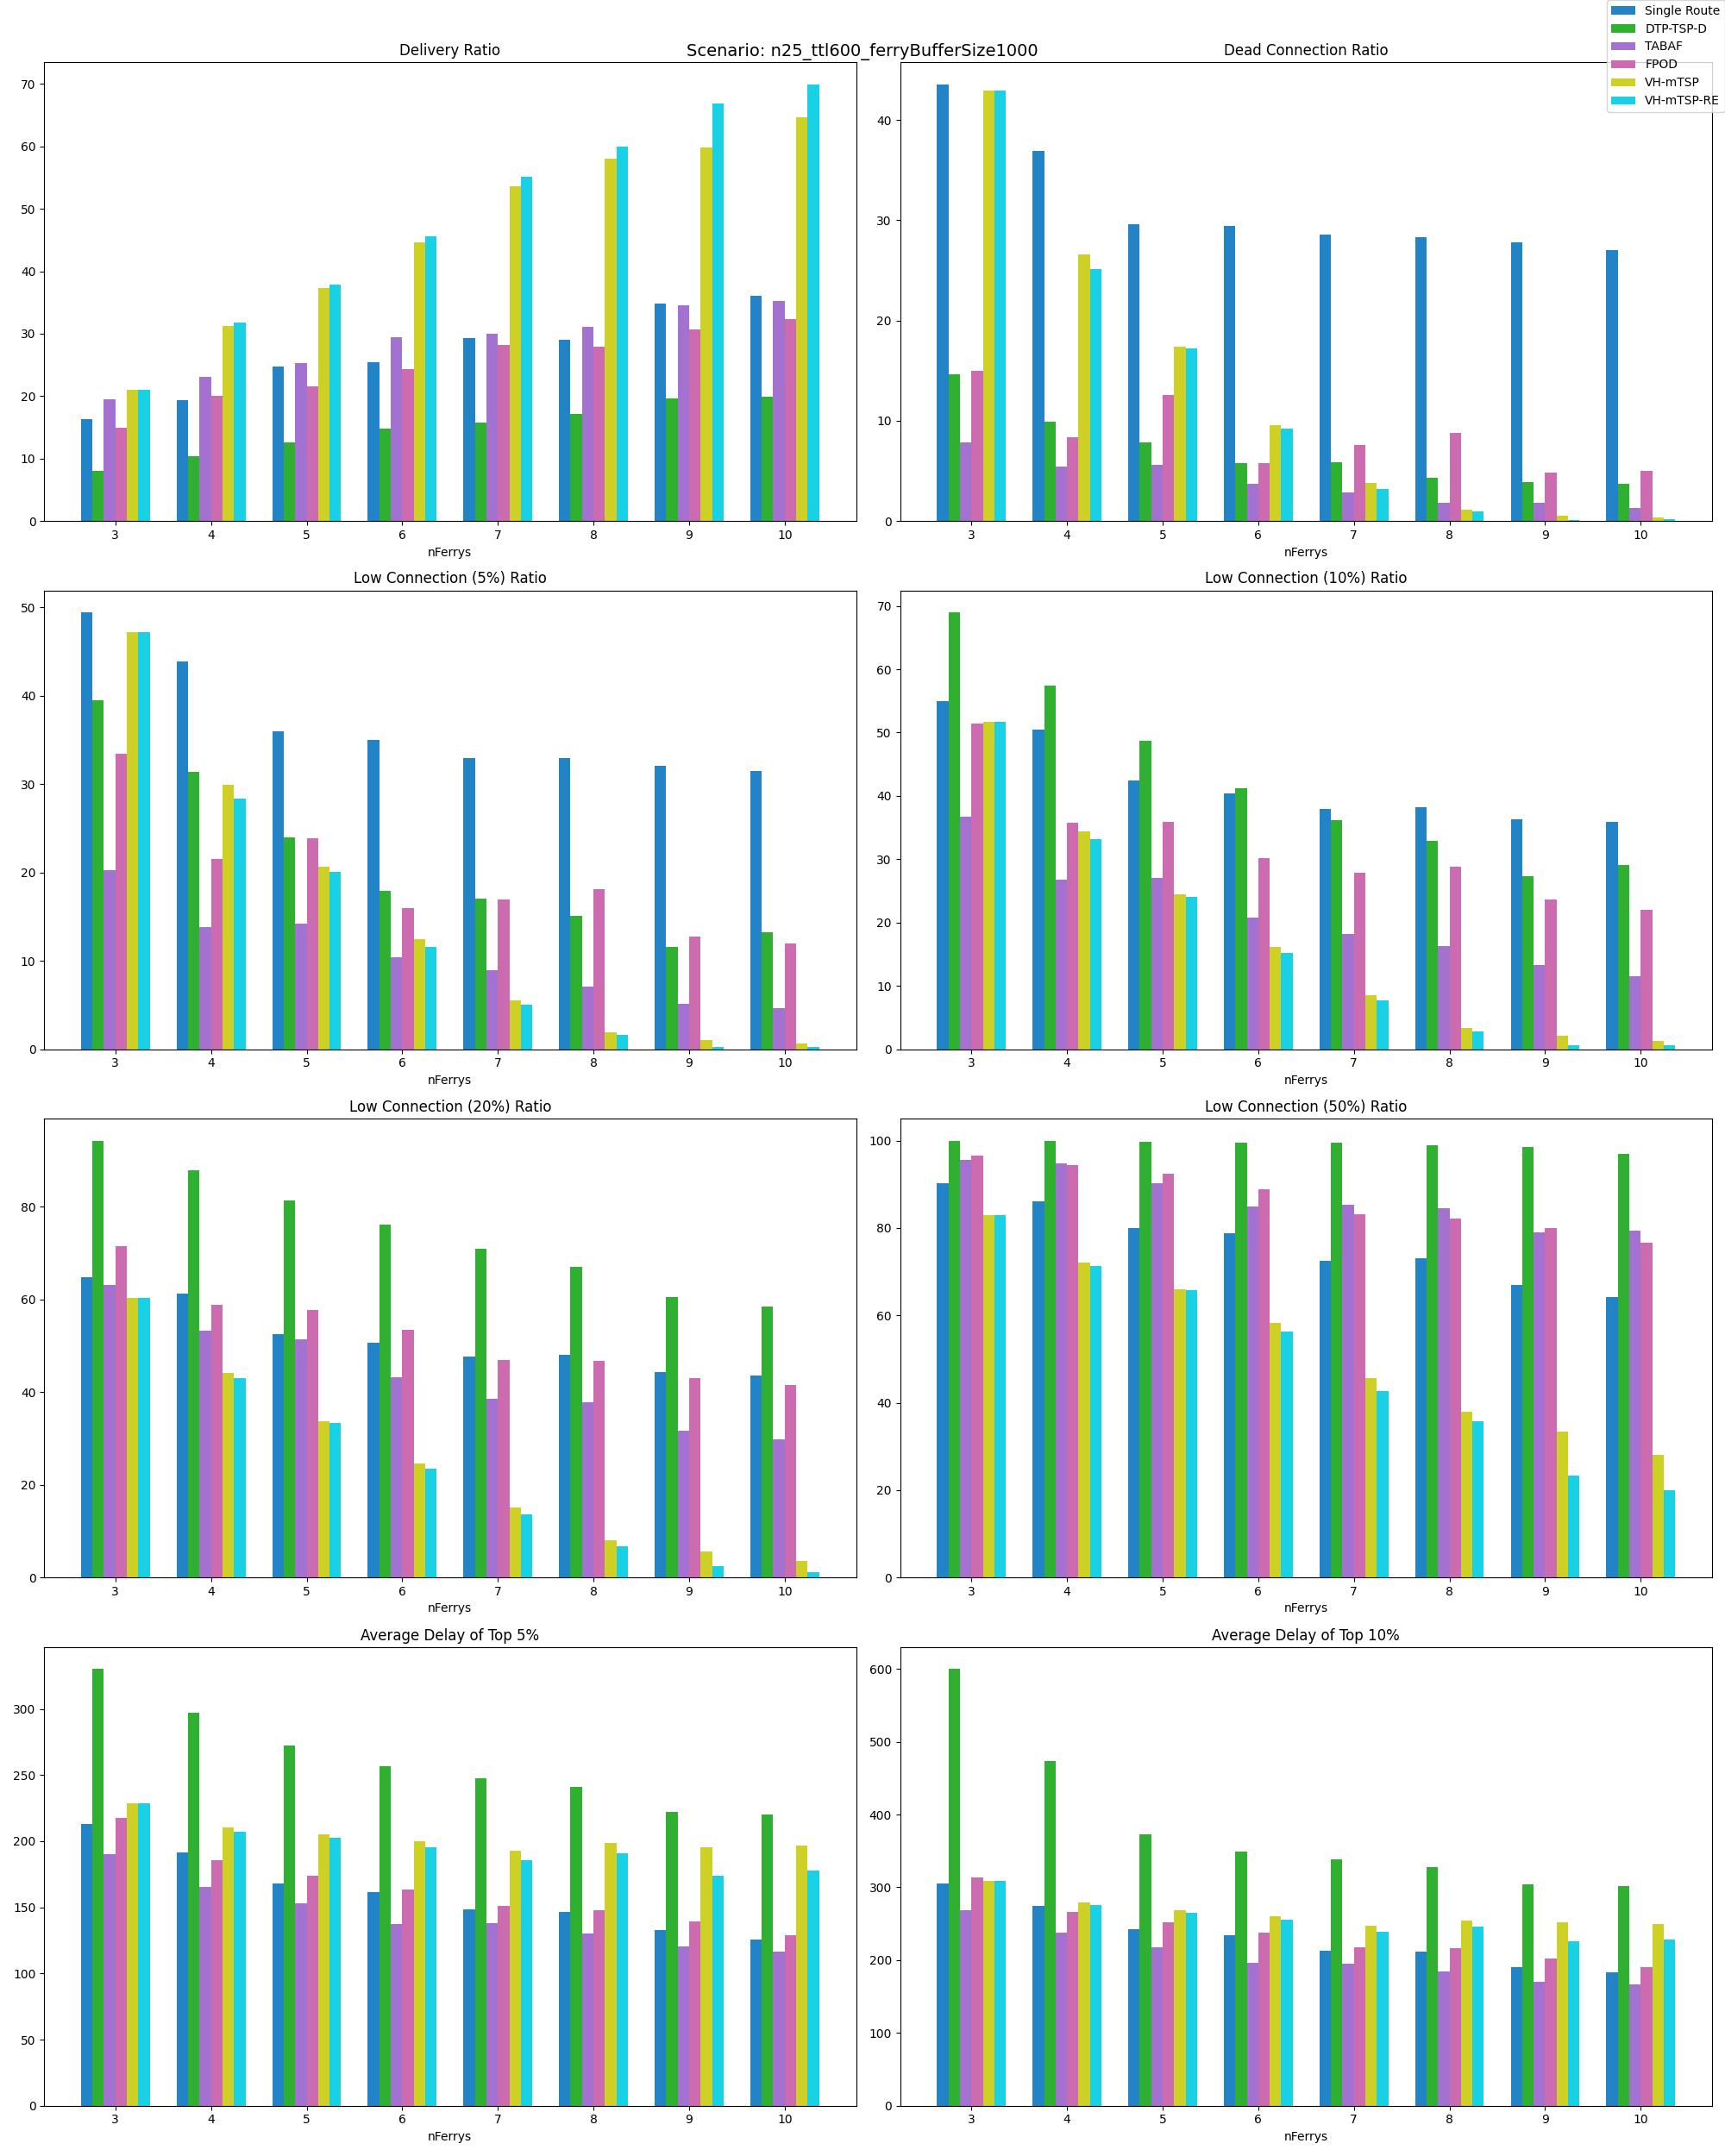
\includegraphics[width=1.0\textwidth]{image/experiment/scenario_n25_ttl600_ferryBufferSize1000.png}
  \caption{Kết quả thực nghiệm kịch bản 1.a}
  \label{fig:1a}
\end{figure}
\begin{figure}[h]
  \centering
  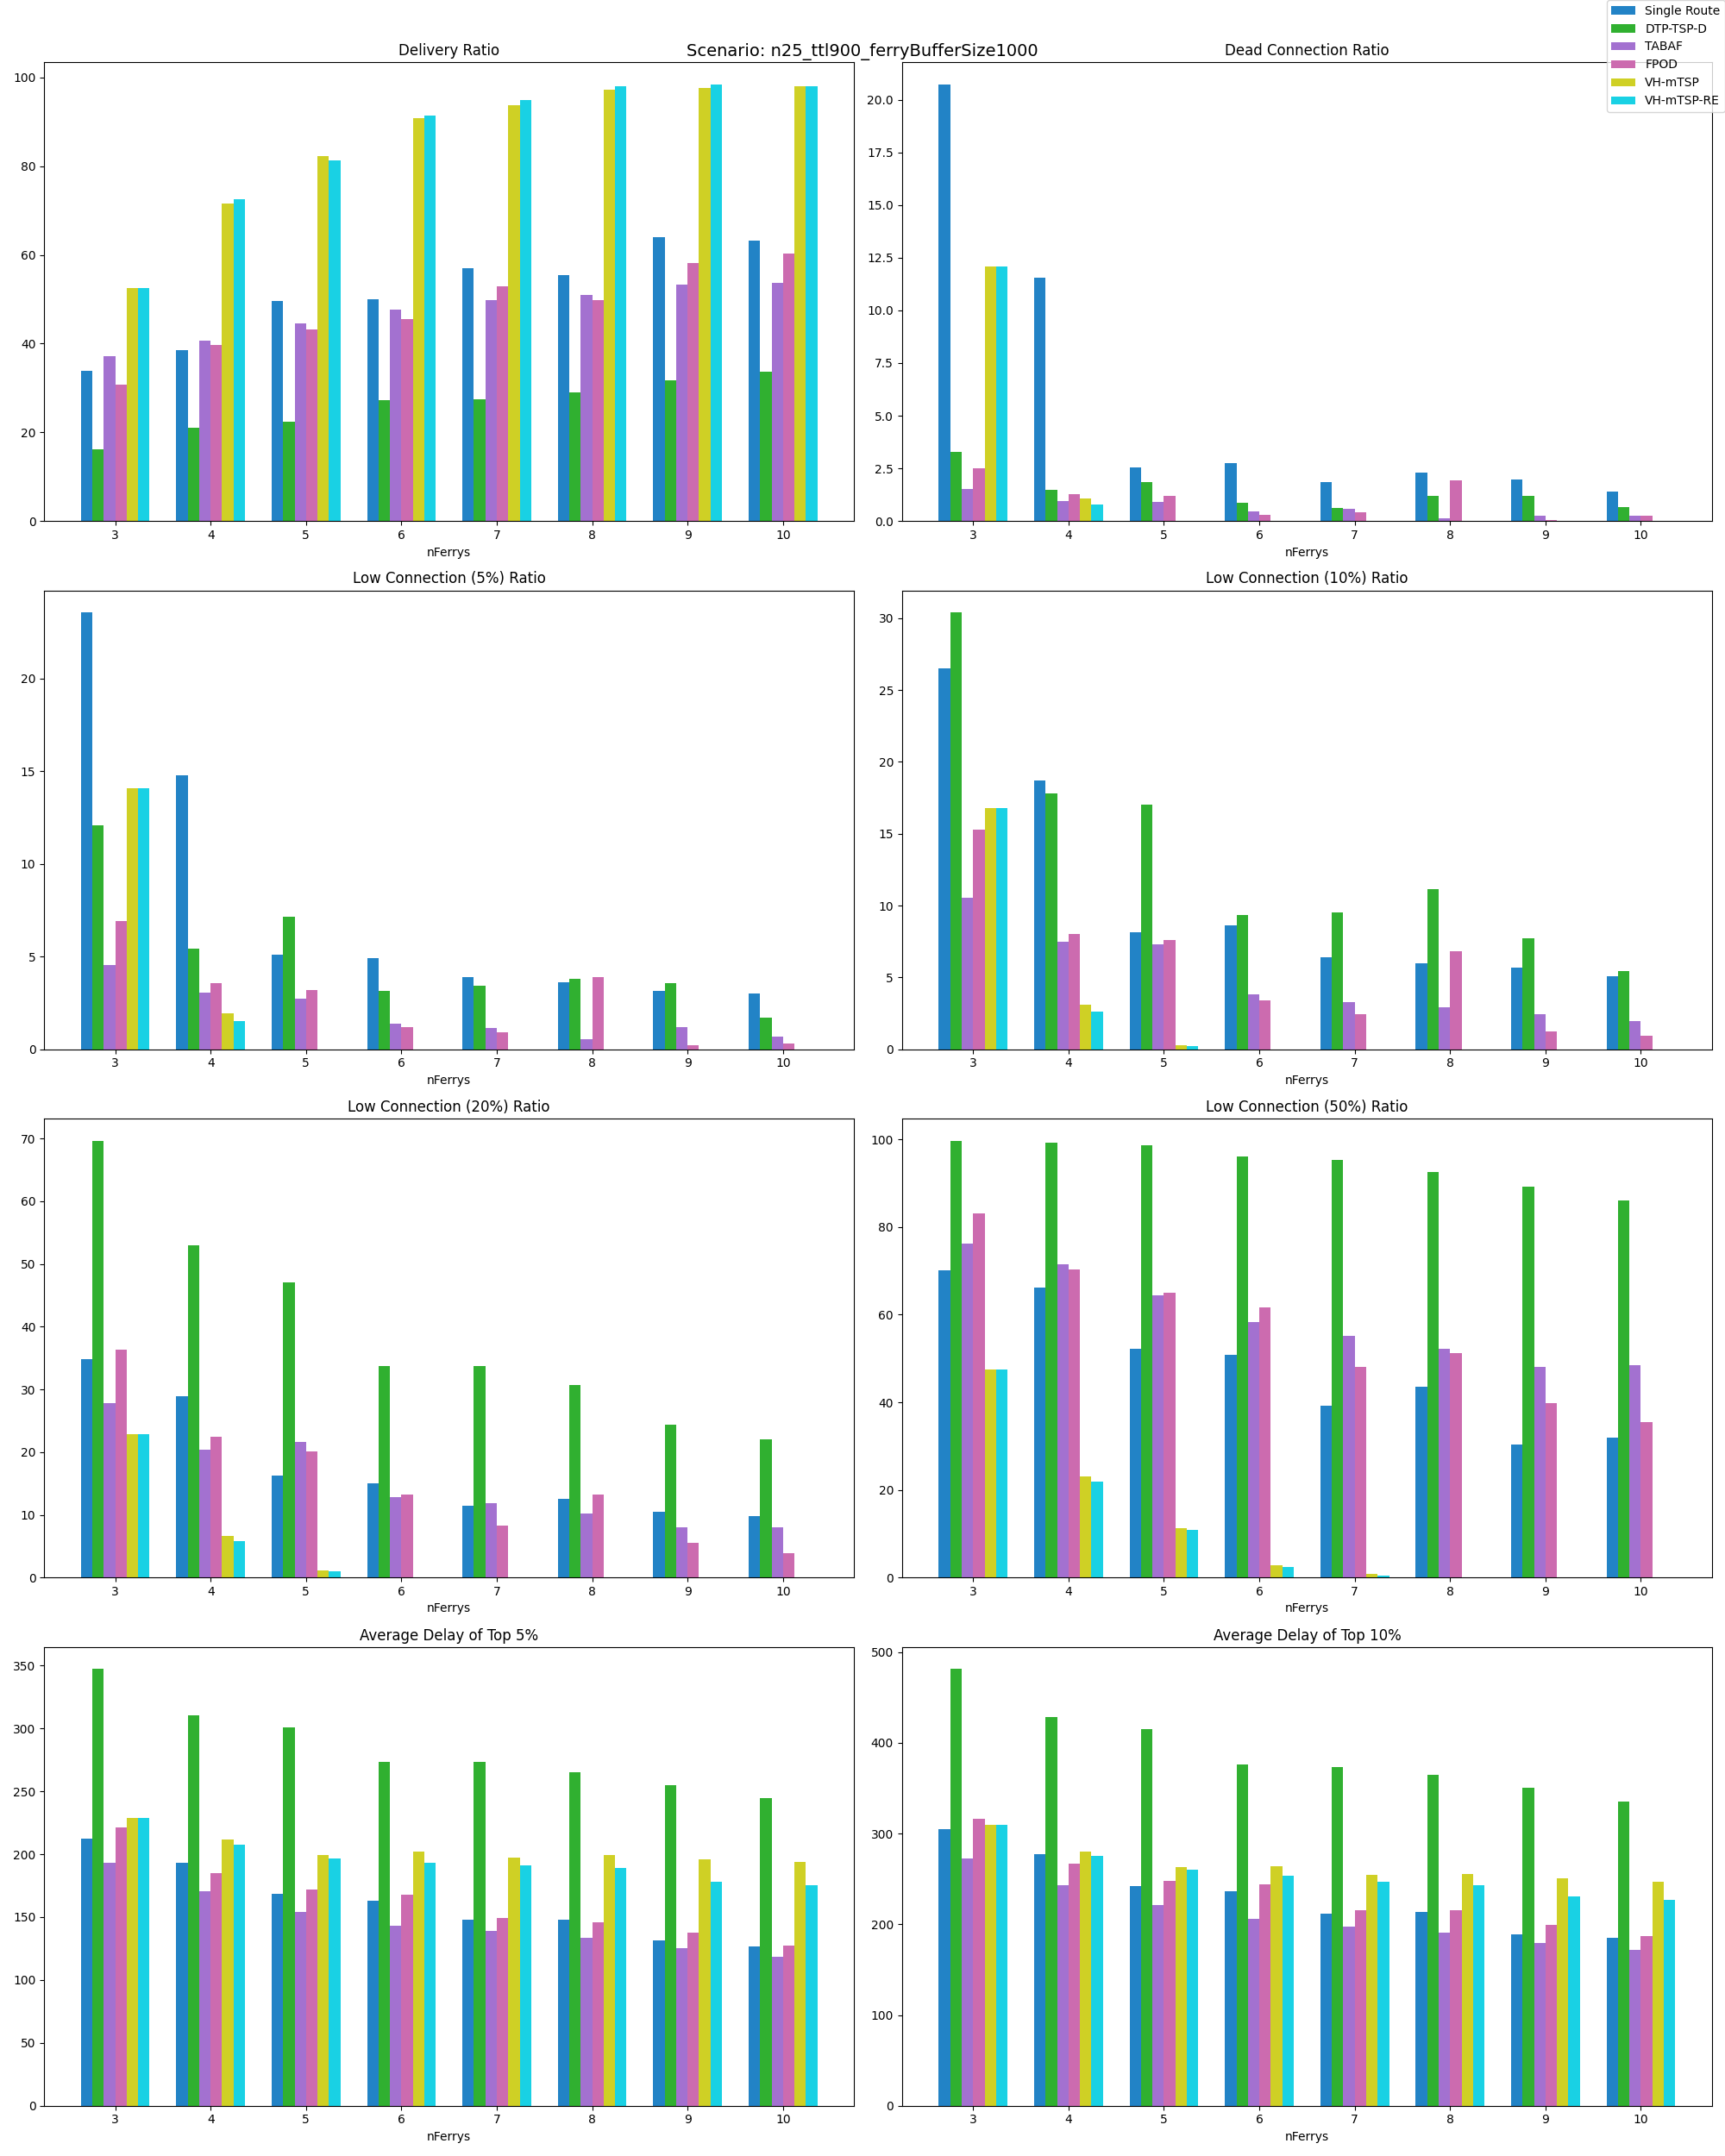
\includegraphics[width=1.0\textwidth]{image/experiment/scenario_n25_ttl900_ferryBufferSize1000.png}
  \caption{Kết quả thực nghiệm kịch bản 2.a}
  \label{fig:2a}
\end{figure}
\begin{figure}[h]
  \centering
  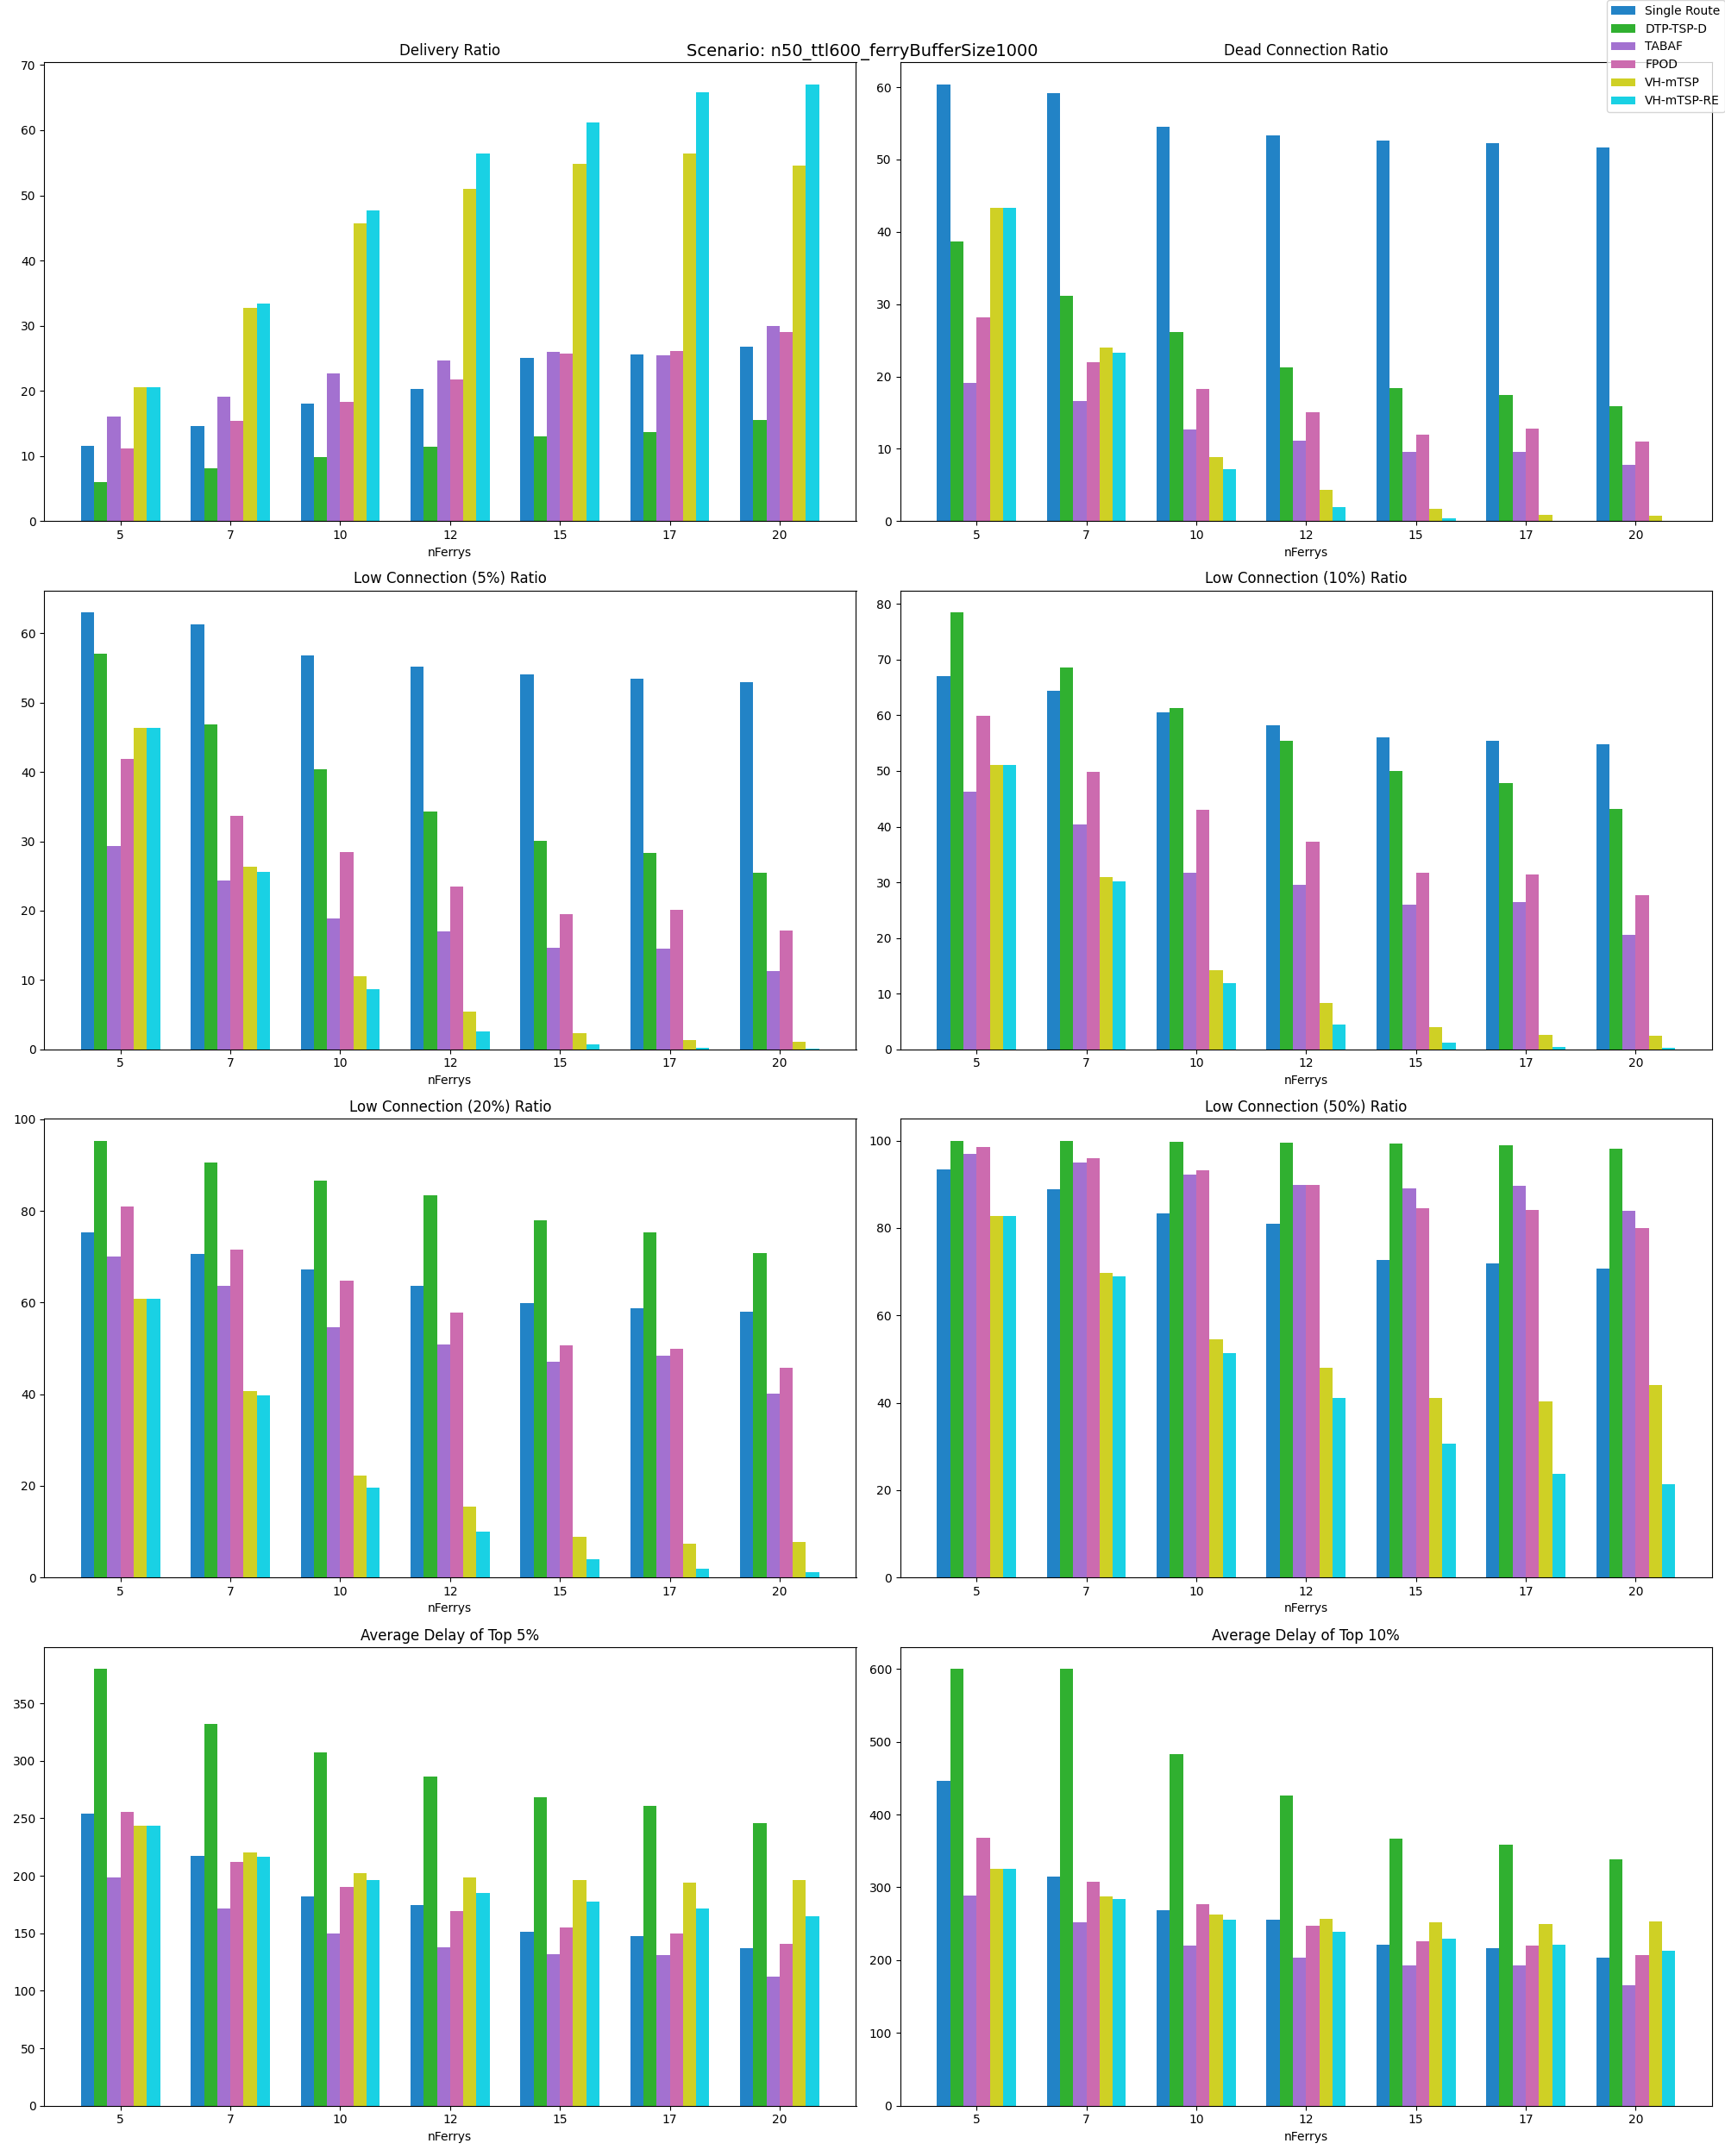
\includegraphics[width=1.0\textwidth]{image/experiment/scenario_n50_ttl600_ferryBufferSize1000.png}
  \caption{Kết quả thực nghiệm kịch bản 3.a}
  \label{fig:3a}
\end{figure}
\begin{figure}[h]
  \centering
  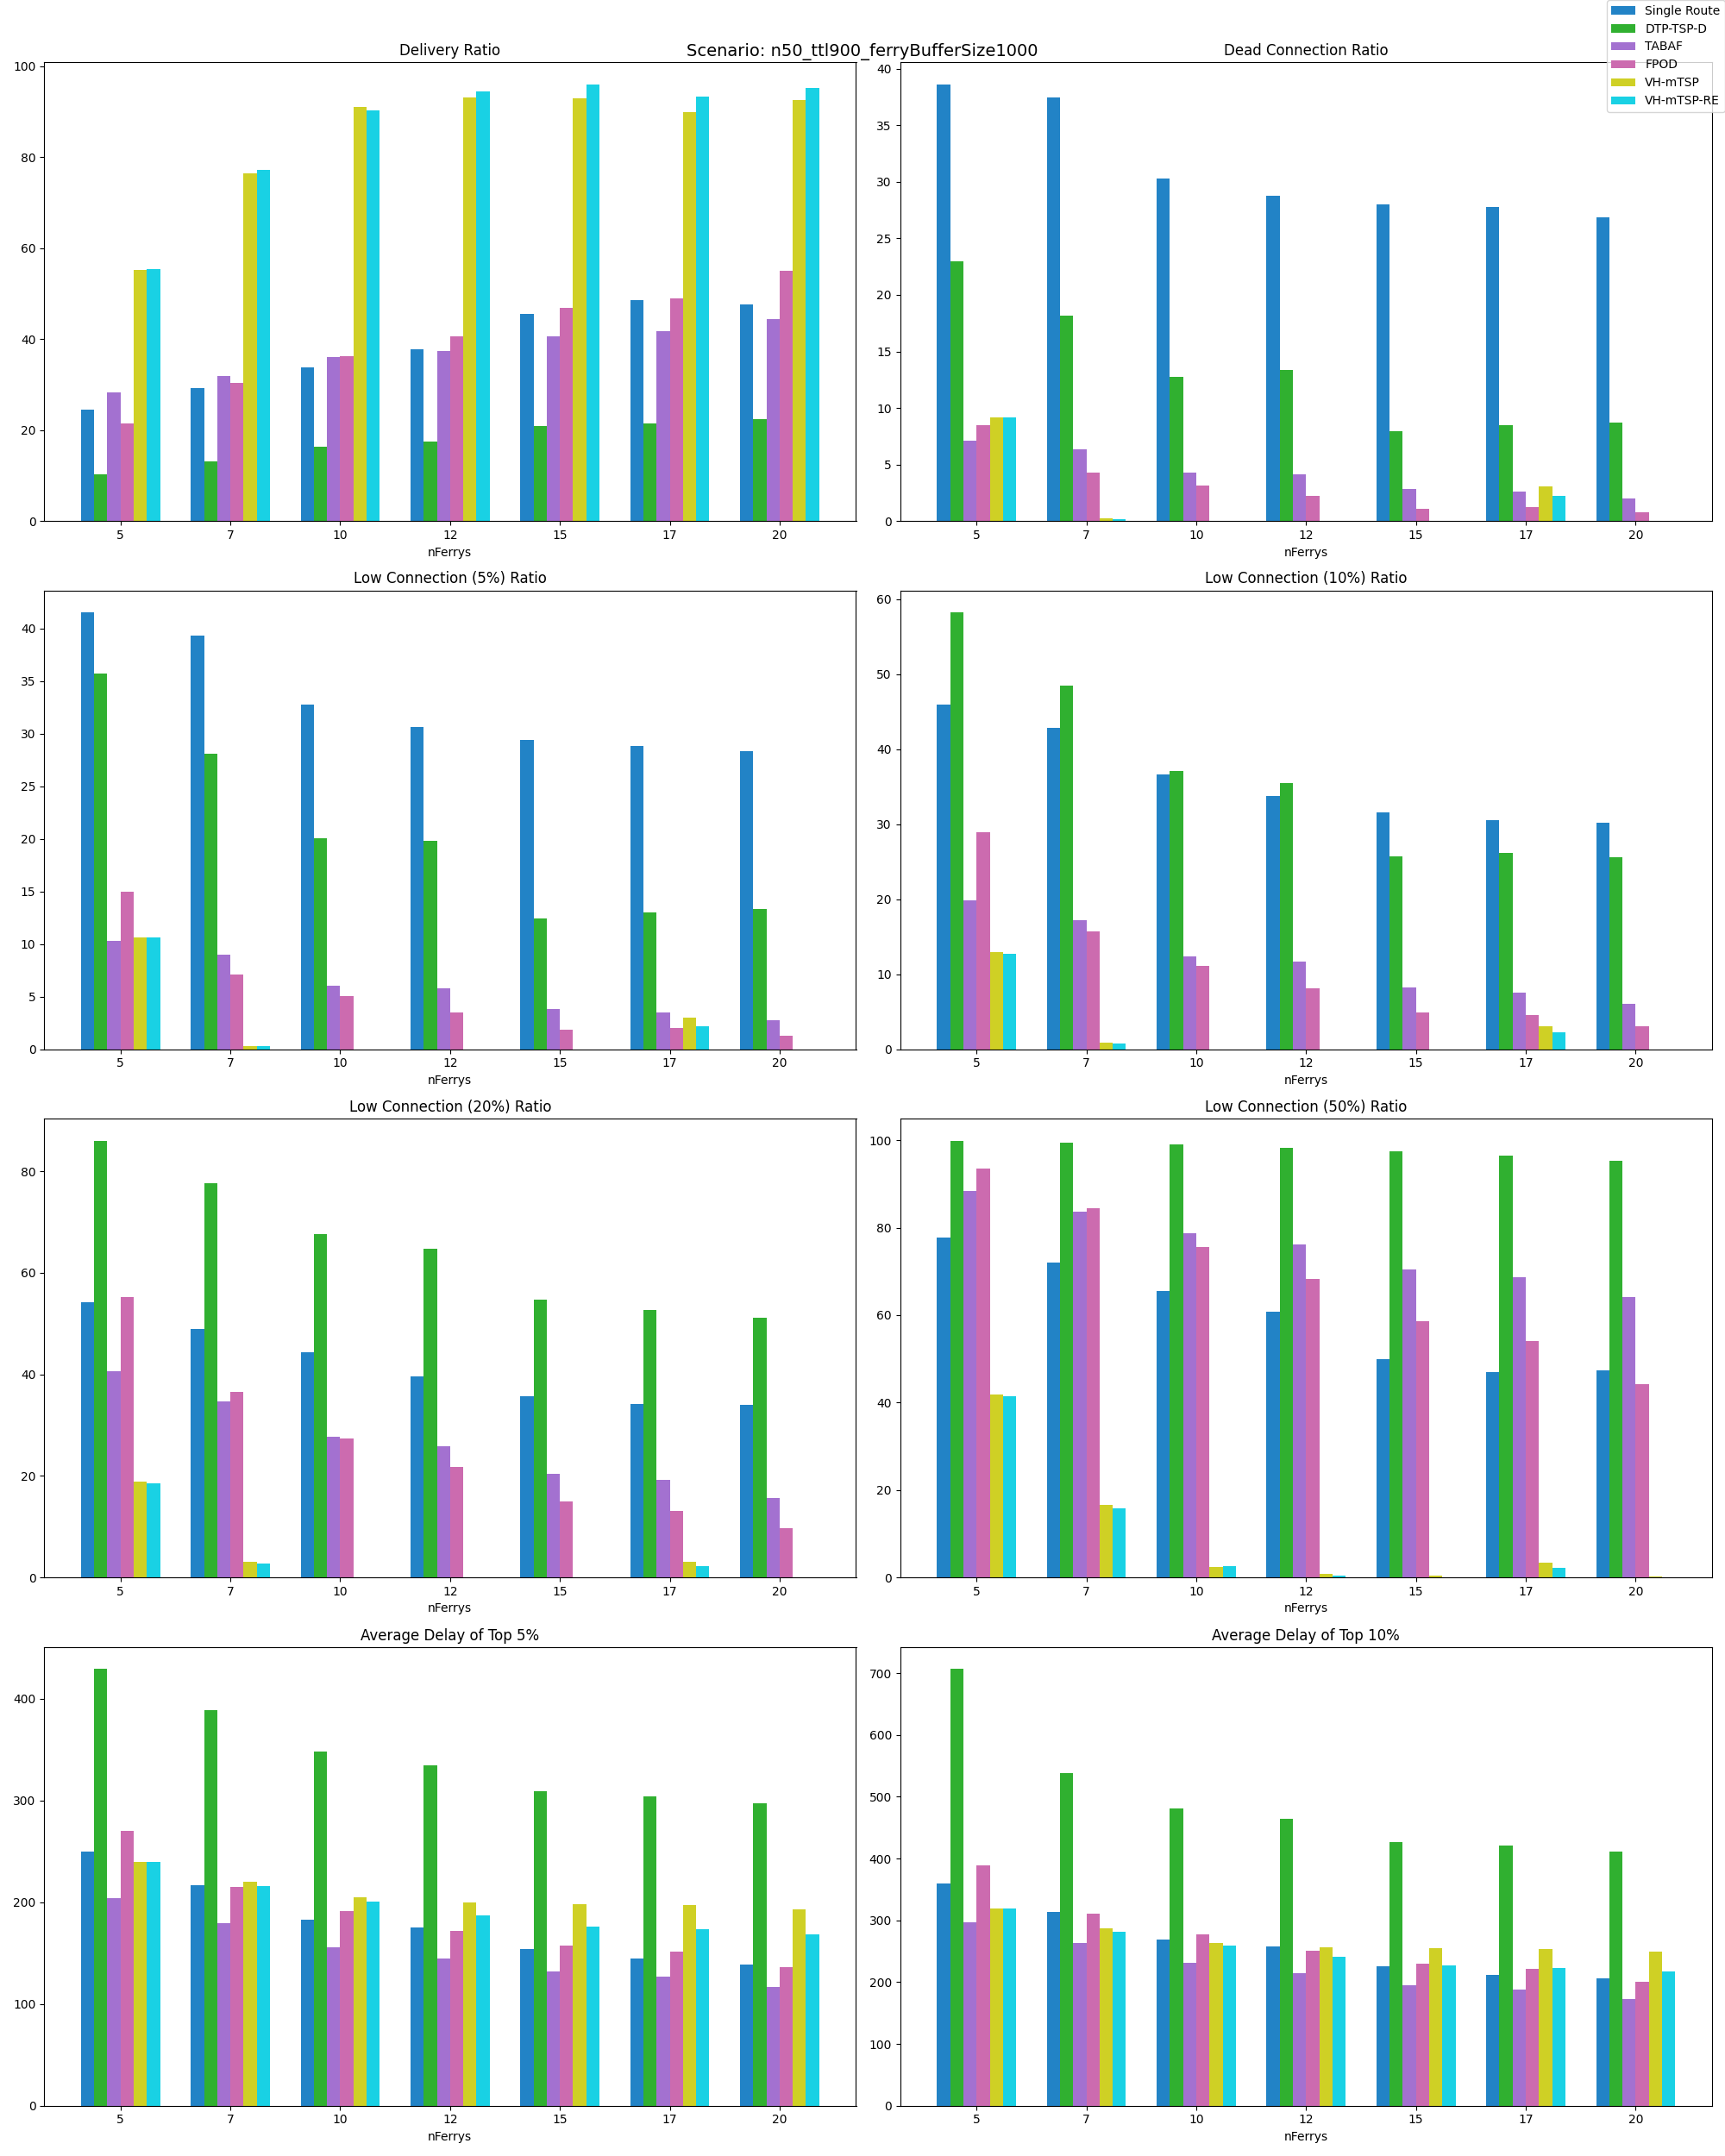
\includegraphics[width=1.0\textwidth]{image/experiment/scenario_n50_ttl900_ferryBufferSize1000.png}
  \caption{Kết quả thực nghiệm kịch bản 4.a}
  \label{fig:4a}
\end{figure}

\subsubsection{Kết quả trên các kịch bản với dung lượng bộ đệm thay đổi}
Nhóm kịch bản này đặt số lượng các UAV ở một mốc cố định và thay đổi dung lượng bộ đệm của các UAV để quan sát và đánh giá.
Biểu đồ chỉ số kết quả thực nghiệm trên các kịch bản 1b, 2b, 3b, 4b lần lượt được thể hiện ở các hình \ref{fig:1b}, \ref{fig:2b}, \ref{fig:3b}, \ref{fig:4b}.

\begin{figure}[h]
  \centering
  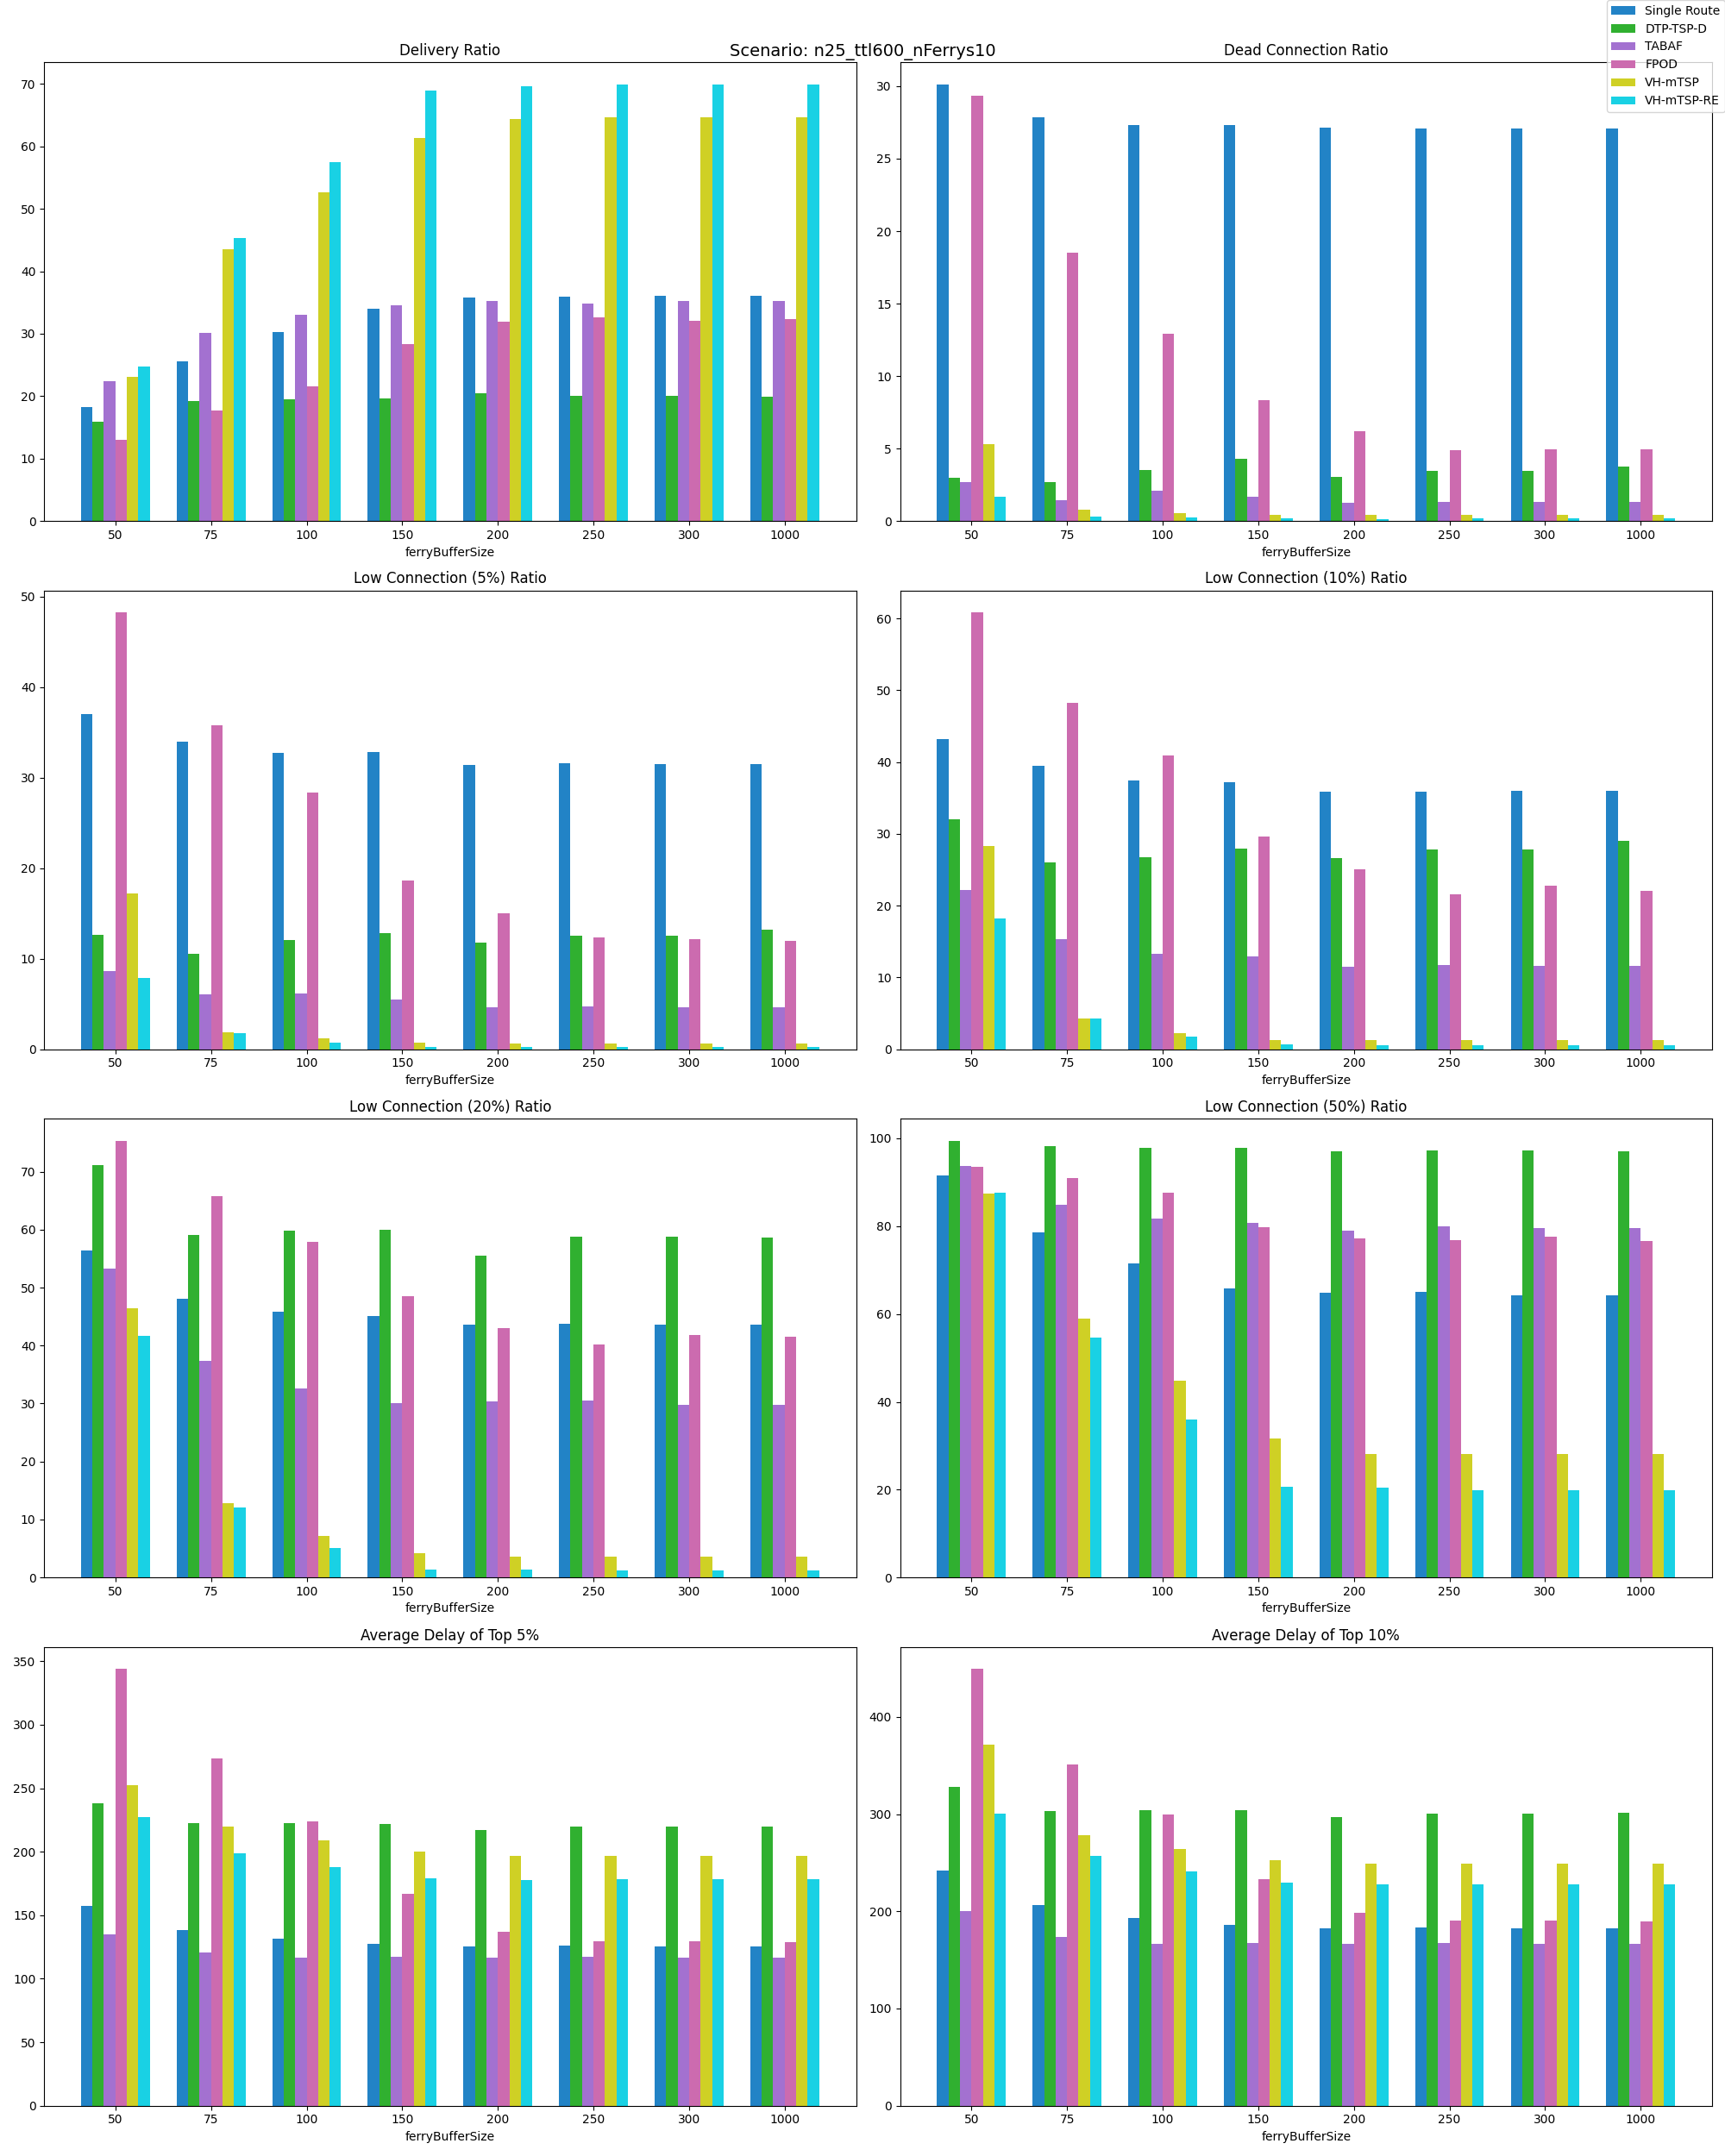
\includegraphics[width=1.0\textwidth]{image/experiment/scenario_n25_ttl600_nFerrys10.png}
  \caption{Kết quả thực nghiệm kịch bản 1.b}
  \label{fig:1b}
\end{figure}
\begin{figure}[h]
  \centering
  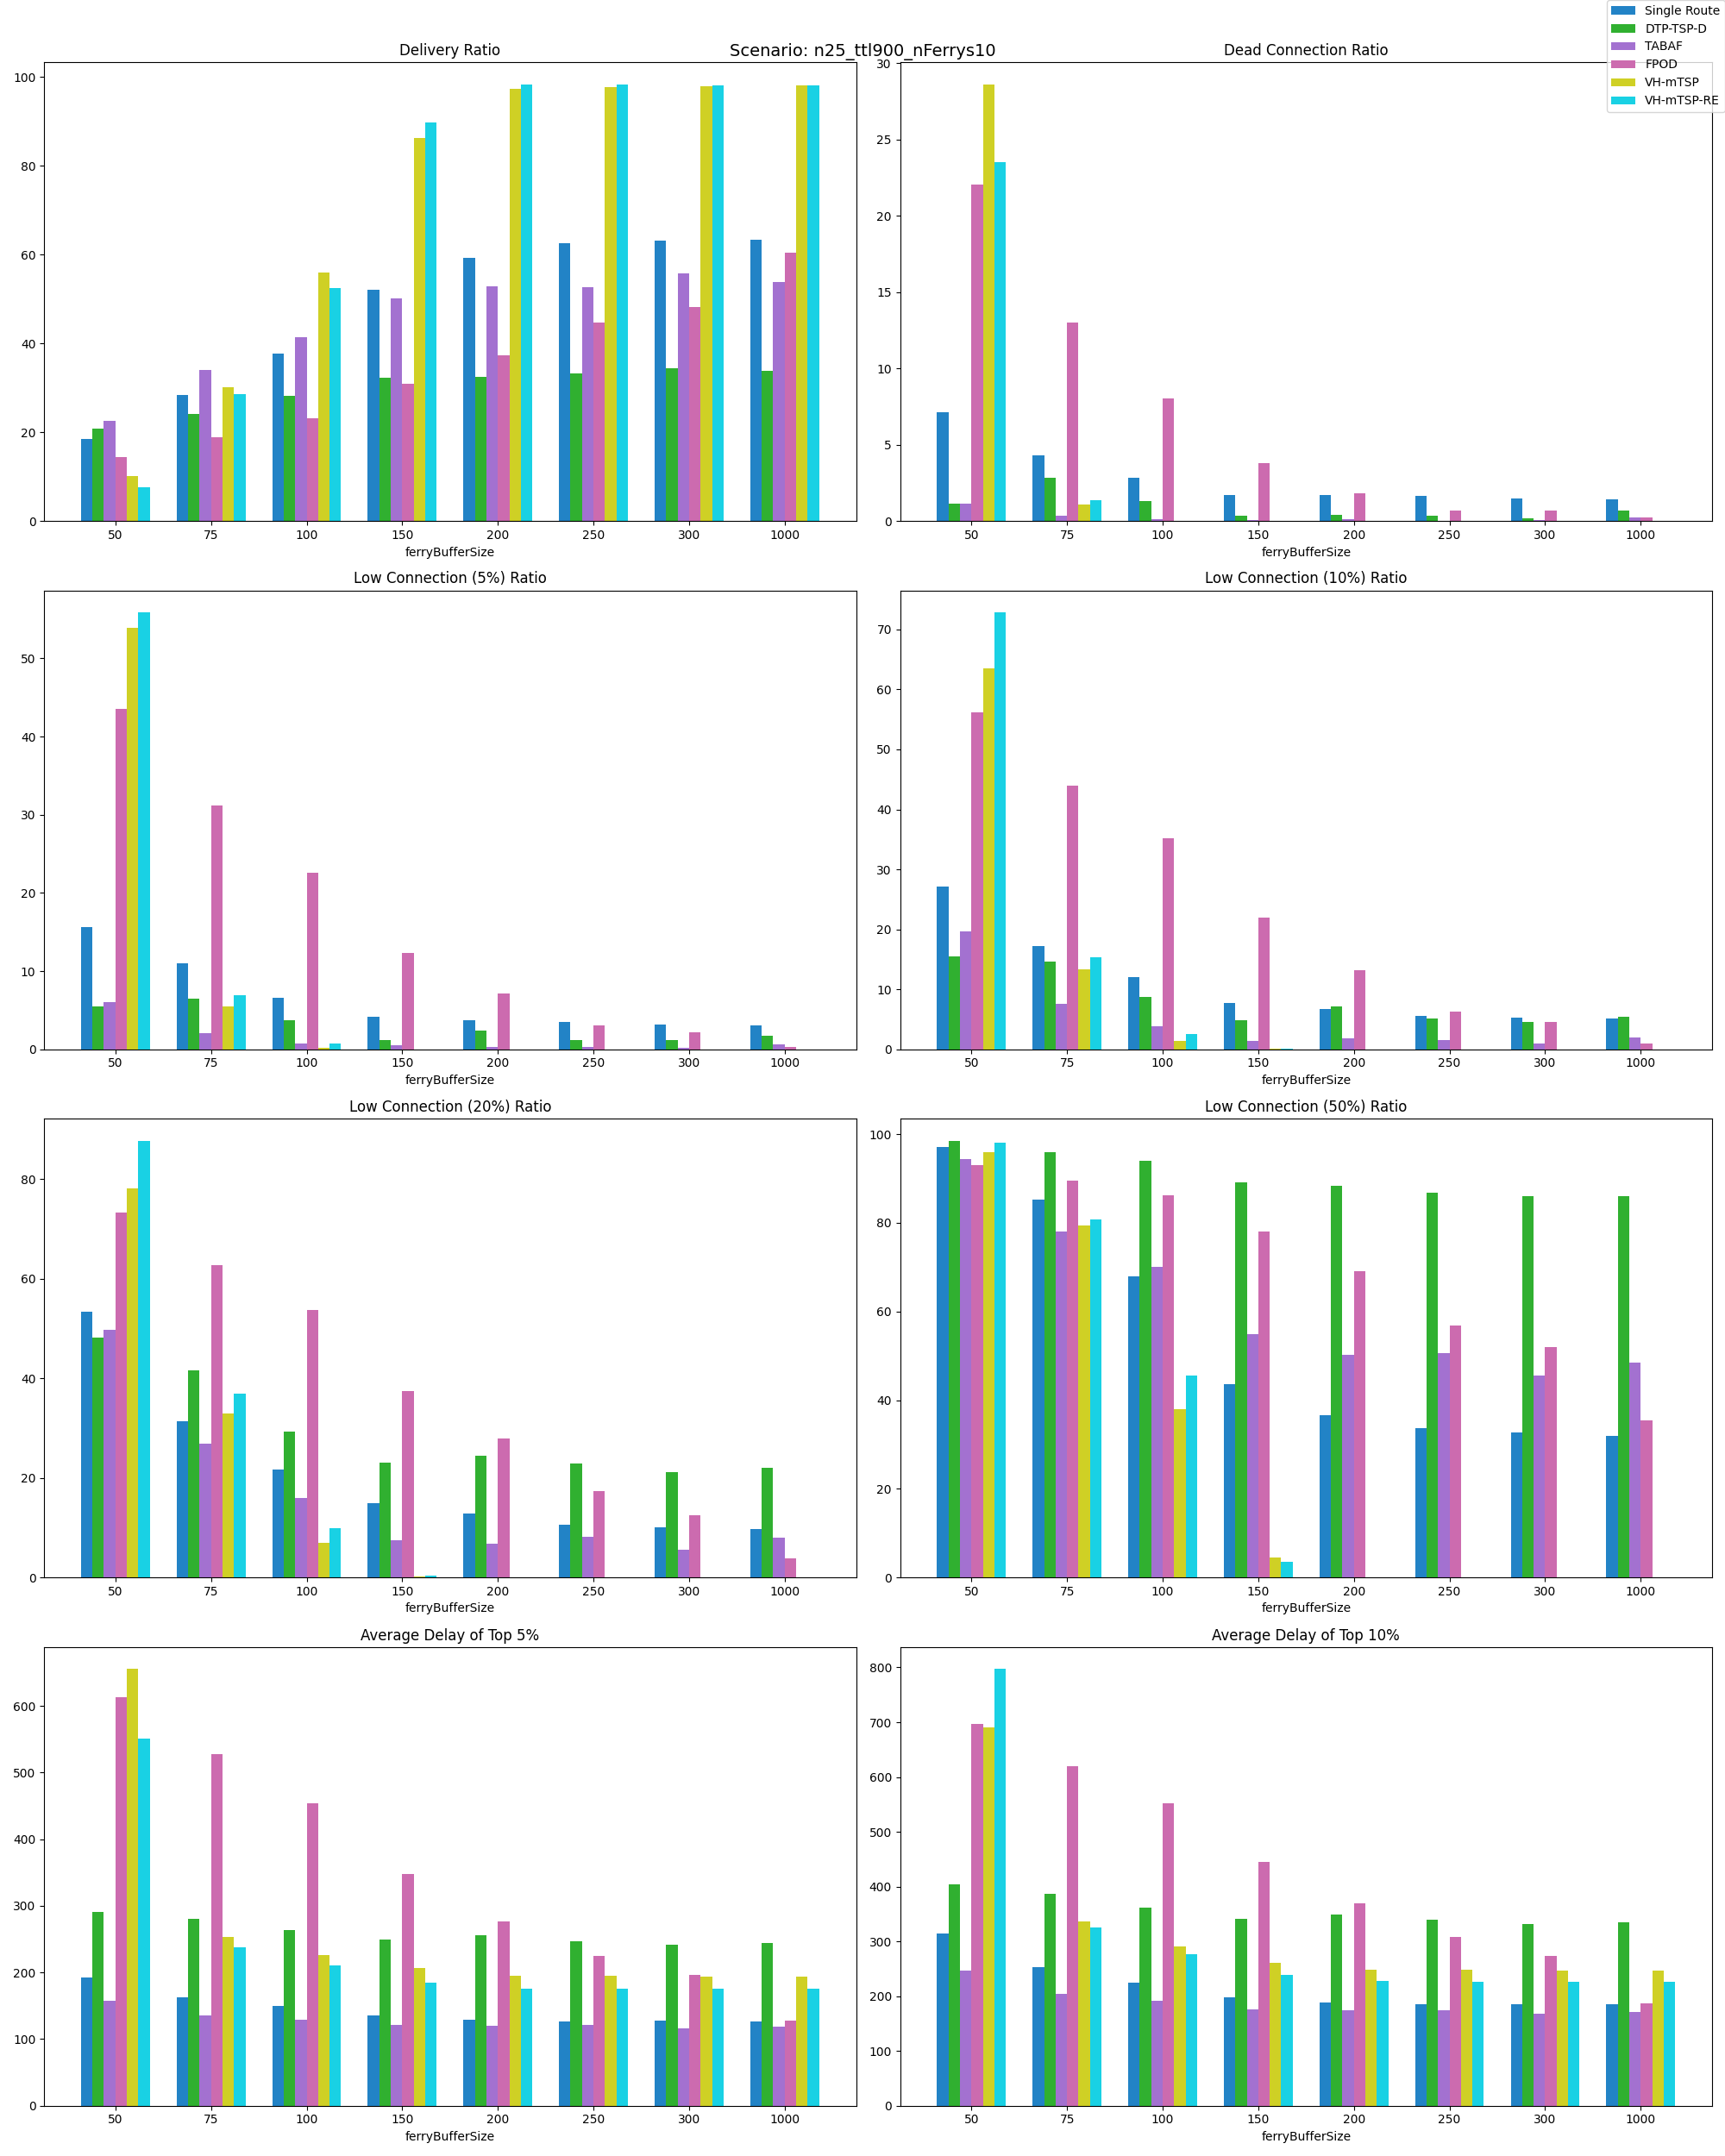
\includegraphics[width=1.0\textwidth]{image/experiment/scenario_n25_ttl900_nFerrys10.png}
  \caption{Kết quả thực nghiệm kịch bản 2.b}
  \label{fig:2b}
\end{figure}
\begin{figure}[h]
  \centering
  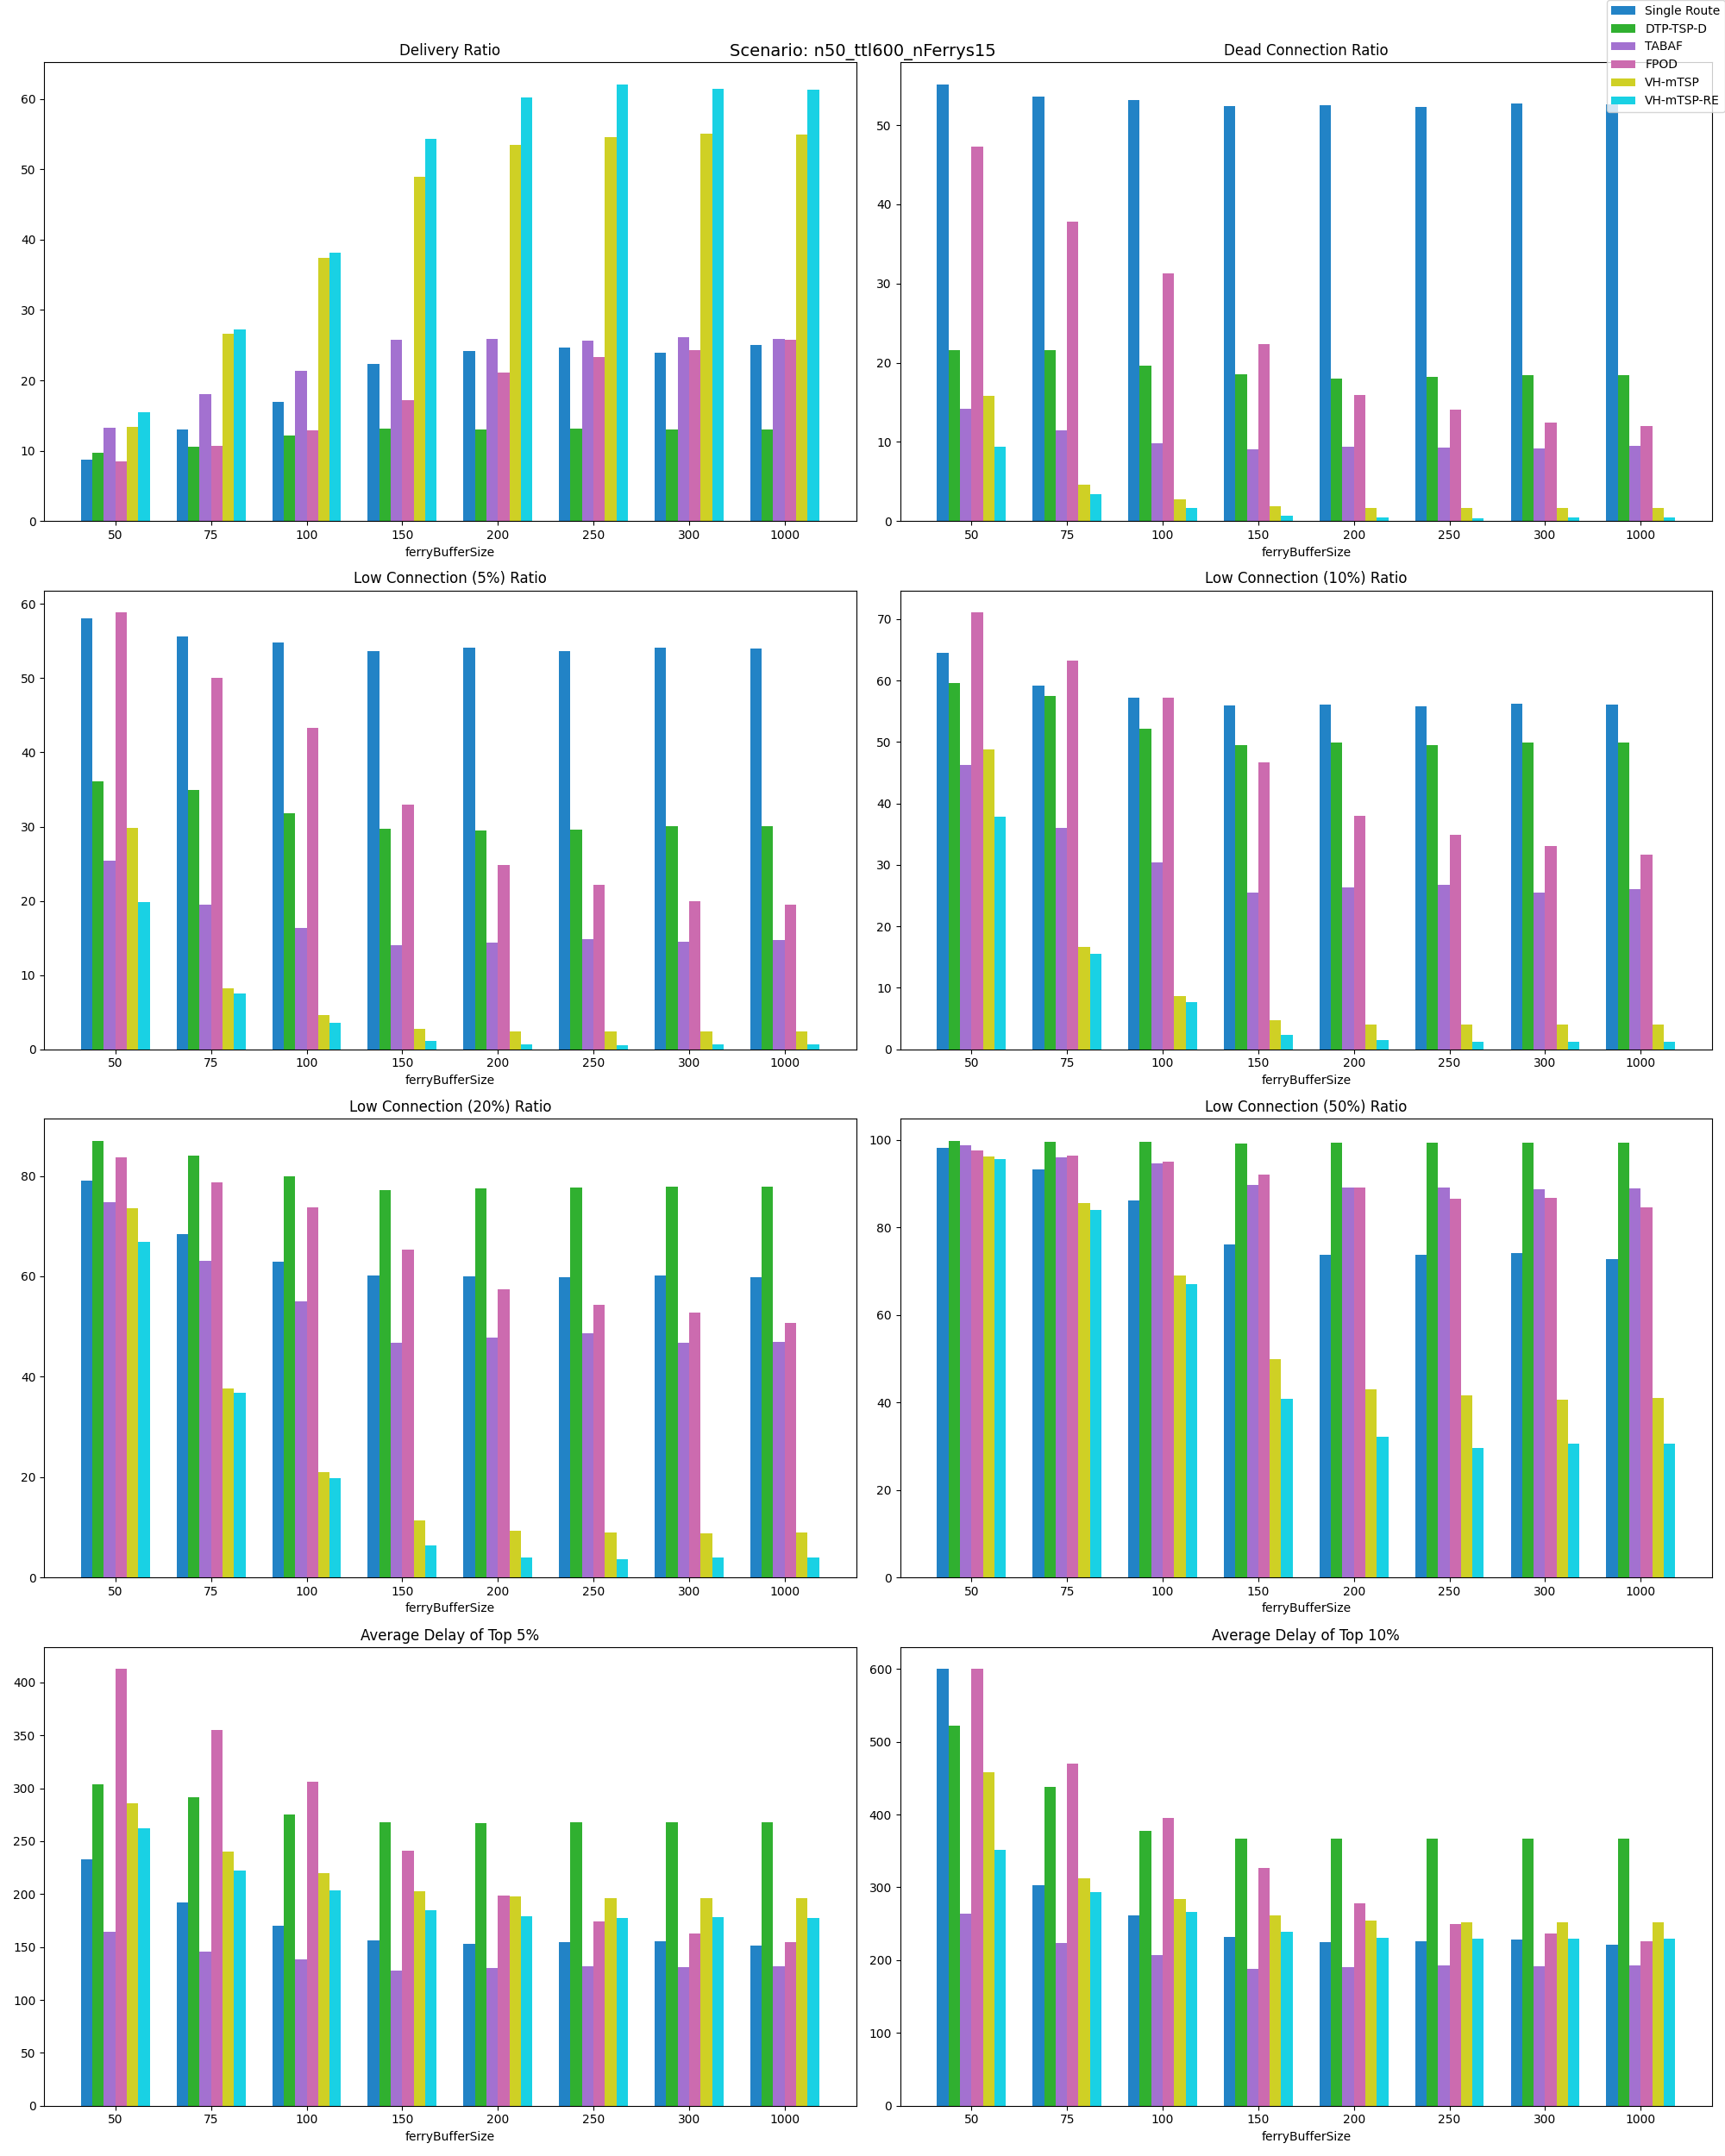
\includegraphics[width=1.0\textwidth]{image/experiment/scenario_n50_ttl600_nFerrys15.png}
  \caption{Kết quả thực nghiệm kịch bản 3.b}
  \label{fig:3b}
\end{figure}
\begin{figure}[h]
  \centering
  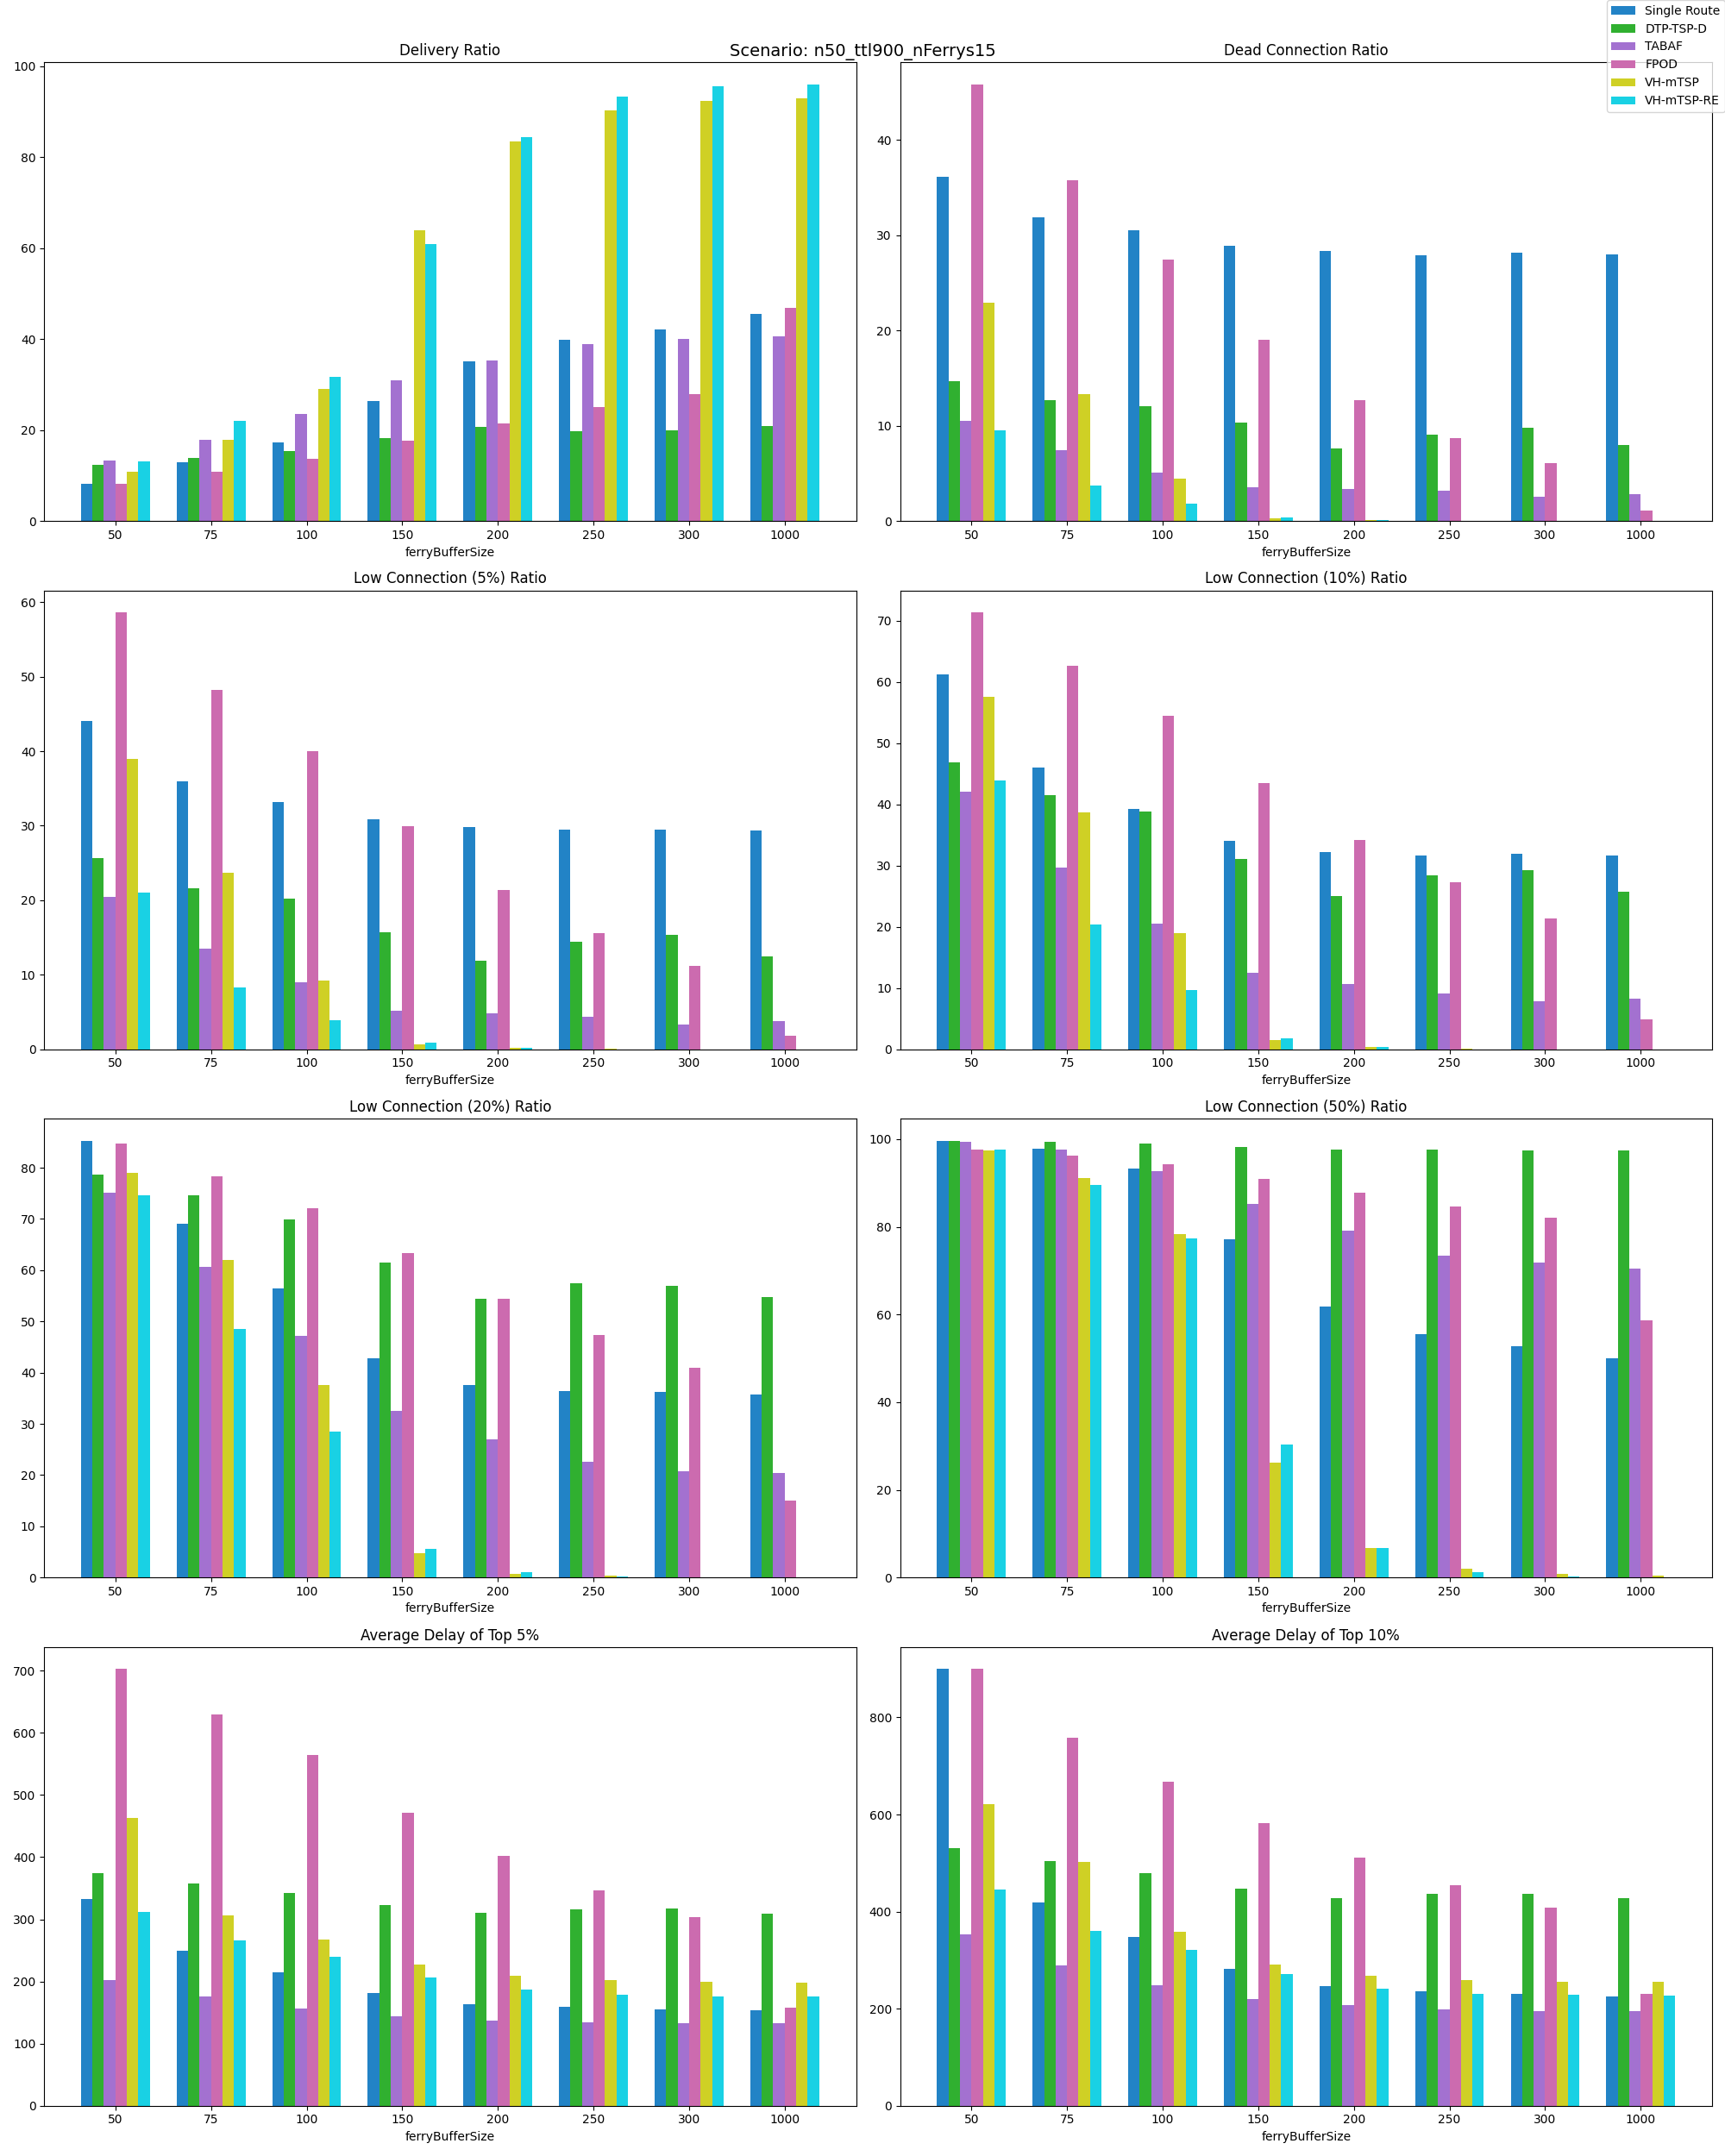
\includegraphics[width=1.0\textwidth]{image/experiment/scenario_n50_ttl900_nFerrys15.png}
  \caption{Kết quả thực nghiệm kịch bản 4.b}
  \label{fig:4b}
\end{figure}
\paragraph{Tổng quan kết quả}

\subsection{Tổng kết chương}

% * Phần 5 ===============================================================
\section{Kết luận và hướng phát triển}
\subsection{Kết luận}
Đề xuất cơ chế trao đổi thông điệp của khóa luận đã đưa ra một cách trao đổi thông điệp giữa các nút mạng trong mạng phà thông điệp, khía cạnh các nghiên cứu trước đây đều chưa đề cập đến. Cơ chế hoạt động hiệu quả trong mô phỏng, thể hiện ở việc các nút mạng có trao đổi được với nhau thì mới thu được các chỉ số như Delivery Ratio hay Dead Connections, \dots Đề xuất có thể trở thành nền tảng quan trọng để ứng dụng triển khai vào thực tế.

Đề xuất quy hoạch lộ trình, định tuyến và lập lịch di chuyển VH-mTSP-RE của khóa luận đã tiếp cận bài toán quy hoạch lộ trình và chuyển tiếp gói tin cho hệ thông đa UAV trong hỗ trợ truyền thông hậu thảm họa một cách có cấu trúc và đảm bảo công bằng giữa các nút mạng. Thuật toán thể thiện rất tốt, vượt xa các giải pháp trước đó như TaBaf, FPOD, DTP-TSP-D về Delivery Ratio, Dead Connection và Low Connection ở nhiều kịch bản. Việc chỉ số Dead Connection đạt 0 ở nhiều kịch bản là minh chứng rõ ràng nhất cho thấy hiệu quả của hướng tiếp cận và là minh chứng chứng minh VH-mTSP-RE có thể được triển khai vào thực tế.

\subsection{Hạn chế}
Mặc dù đề xuất VH-mTSP-RE của khóa luận đã đạt được những kết quả tốt trong môi trường mô phỏng, nó vẫn tồn tại những hạn chế:
\begin{itemize}
  \item Trong các kịch bản khó, có ít UAV và thời gian sống của thông điệp thấp, hiệu năng của thuật toán giảm rõ rệt, đặc biệt thể hiện ở chỉ số Dead Connection Ratio rất cao. Điều này là do khi có ít UAV, các UAV đều phải phục vụ nhiều nút, khiến thời gian các UAV hoàn thành một vòng lộ trình (đi từ điểm trung chuyển đến các nút mặt đất và quay lại) rất lâu, thậm chí lớn hơn thời gian sống của một thông điệp.
  \item Thuật toán chưa có cơ chế để thêm hoặc bớt nút mạng trong quá trình chạy, khi thay đổi số lượng UAV hoặc nút mặt đất thì chỉ có cách chạy lại thuật toán từ đầu, mà việc các chạy thuật toán tối ưu hóa để tìm lộ trình mới sẽ tốn thời gian. Trong khi đó phương pháp TaBaf hay FPOD có thể thêm bớt trong quá trình chạy mà không mất thêm thời gian tính toán.
  \item Việc nhiều UAV tập hợp lại một chỗ để trao đổi có thể gây nhiễu và xung đột khi trao đổi trong thực tế, khi triển khai đề xuất trong mối trường thực tế thì các UAV có thể phải chờ tại điểm trung chuyển một thời gian lâu hơn để có thể trao đổi, làm giảm hiệu năng. Do đó, cần có các thực nghiệm thực tế để xác định mức độ ảnh hưởng và đề xuất giải pháp.
  \item Giao thức trao đổi thông điệp hiện vẫn chỉ được cài đặt ở mức mô phỏng, chưa xét đến toàn bộ đặc tả kỹ thuật của Bundle Protocol được mô tả trong RFC 5050 và RFC 9171.
\end{itemize}
\subsection{Hướng nghiên cứu tiếp theo}
Các hạn chế được chỉ ra ở mục trước là nền tảng đề xuất các hướng nghiên cứu và phát triển tiếp theo:
\begin{itemize}
  \item {\bfseries Hoàn thiện mô phỏng:} Các kịch bản mô phỏng cần thực tế hơn, sử dụng các mô hình truyền dẫn đúng với yêu cầu thực tế. 
  \item {\bfseries Hoàn thiện hệ thống:} Phát triển quy trình để việc giải bài toán trở thành một luồng thống nhất: Từ vị trí các nút mặt đất đến việc tìm các điểm đại diện, đến việc triển khai quy hoạch lộ trình. Bên cạnh đó là phát triển giao thức giao đổi sao cho thực tế hơn, các thông điệp sẽ có độ lớn khác nhau và cần tính năng phân mảnh.
  \item {\bfseries Tích hợp triển khai trong thực tế:} Từ các kết quả đạt được trong mô phỏng, hướng phát triển tự nhiên nhất của khóa luận là việc tích hợp và triển khai VH-mTSP-RE trong thực tế. Việc này không chỉ bao gồm cài đặt các thuật toán đã nêu, mà còn phải xét đến các yếu tố mối trường, như nhiễu, gió, thời tiết, vật cản, ngoài ra còn phải giải quyến bài toán tránh va chạm cho các UAV.
  \item {\bfseries Nghiên cứu thuật toán quy hoạch lộ trình và định tuyến cho các kịch bản khó:} VH-mTSP-RE đã tiếp cận đề tài theo một hướng có cấu trúc và công bằng, nhưng với các kịch bản có ít UAV và thời gian sống của thông điệp thấp, ta có thể sẽ cần một hướng tiếp cận khác. 
\end{itemize}

% \newpage
\renewcommand{\refname}{\vspace{-1cm}}
\section*{Tài liệu tham khảo}
\addcontentsline{toc}{section}{Tài liệu tham khảo}
\printbibliography
\end{document}